\documentclass[english]{amu_these}

\begin{document}

										%% page de titre
	\chead{}
	\pdfbookmark[0]{Page de titre}{titre}
	\thispagestyle{empty}
	\newgeometry{margin=2em}

\begin{center}
	\begin{minipage}[c]{.5\linewidth}
		\raggedright
\includegraphics[height=7em]{logo_amu_excellence}
	\end{minipage}\hfill
	\begin{minipage}[c]{.5\linewidth}
		%\raggedleft\includegraphics[height=7em]{example-image-b} %% logo cotutelle
	\end{minipage}\hfill
\end{center}

\vspace{1em}

\begin{center}
	\begin{minipage}[c]{.63\linewidth}
		\dhorline{\textwidth}{4pt}
	\end{minipage}\hfill
	\begin{minipage}[c]{.35\linewidth}
		\raggedleft\titl{NNT/NL : 2020AIXM0001/001ED000}
		% renseigner votre numéro national de thèse (NNT) et le numéro local (NL)
		% ils sont indiqués sur la page d'informations administratives de votre espace de dépôt dans le guichet de dépôt légal des thèses AMU lorque votre date de soutenance est renseignée par votre service de scolarité
		% https://depot-theses.univ-amu.fr/
	\end{minipage}\hfill
\end{center}

%\vspace{1em}

\doublespacing
\begin{flushleft}
    \titb{\HUGE\textcolor{cyanamu}{Habilitation à Diriger des Recherches}}\\
	\titl{\Large Présentée à Aix-Marseille Université}\\
	%\titl{\Large dans le cadre d'une cotutelle avec }\\
	\titl{\Large le XX janvier 2022 par}\\
\end{flushleft}
\vspace{2em}
\begin{center}
	\titsb{\Huge Julián Ernesto BAUTISTA}\\
    \vspace{1em}
	\titm{\LARGE dark energy with Spectroscopic Observations of the Universe}\\
\end{center}
\singlespacing

\vspace{4em}

\begin{center}
	\begin{minipage}[t]{.45\linewidth}
    	    \vspace{.5em}
        	\titb{Discipline}
        	
        	\titl{Physique et Sciences de la Matière}
        	
    	    \vspace{1em}
        	\titb{Spécialité}
        	
        	\titl{Astrophysique et Cosmologie}
        	
    	    \vspace{1em}

        	\titb{Laboratoire}
        	
        	\titl{Centre de Physique des Particules de Marseille
        	}
	\end{minipage}\hfill
	\begin{minipage}[t]{.03\linewidth}
	    \dvertline{4pt}{-16em}
	\end{minipage}\hfill
	\begin{minipage}[t]{.52\linewidth}
	    \vspace{.5em}
    	\titb{Composition du jury}

	    \vspace{1em}
    	\titl{
        \begin{tabular}{p{12em} p{9.5em}}
        	Prénom NOM & Rapporteur·e \\
        	Affiliation \\
        	\\
        	Prénom NOM & Rapporteur·e \\
        	Affiliation \\
            \\
            Prénom NOM & Examinateur·rice \\
        	Affiliation \\
            \\
        	Prénom NOM & Président·e du jury \\
        	Affiliation \\
            \\
        	Prénom NOM & Tuteur \\
        	Affiliation \\
        \end{tabular}
        }
	\end{minipage}\hfill
\end{center}       

\vspace{2em}

\begin{center} %% logos partenaires
	\begin{minipage}[c]{.25\linewidth}
		\centering\includegraphics[height=5em]{example-image-a} 
	\end{minipage}\hfill
	\begin{minipage}[c]{.25\linewidth}
		\centering\includegraphics[height=5em]{example-image-b}
	\end{minipage}\hfill
	\begin{minipage}[c]{.25\linewidth}
		\centering\includegraphics[height=5em]{example-image-c} 
	\end{minipage}\hfill
	\begin{minipage}[c]{.25\linewidth}
		\centering\includegraphics[height=5em]{example-image-c}
	\end{minipage}\hfill
\end{center}

\restoregeometry
										%% licence
	\newpage
	\pdfbookmark[0]{Affidavit}{affidavit}
	\thispagestyle{empty}
	\iftrue % Déclaration sur l'honneur pour une thèse en français (inverser les \if pour une thèse en anglais)
    Je soussigné, Julián Ernesto BAUTISTA, %% Prénom et Nom de l'auteur %%
    déclare par la présente que le travail présenté dans ce manuscrit est mon propre travail, 
    dans le respect des principes d'honnêteté, d'intégrité et de responsabilité inhérents à la mission de recherche. Les travaux de recherche et la 
    rédaction de ce manuscrit ont été réalisés dans le respect à la fois de la charte nationale de déontologie des métiers de la recherche et de la 
    charte d'Aix-Marseille Université relative à la lutte contre le plagiat.
    
    Ce travail n'a pas été précédemment soumis en France ou à l'étranger dans une version identique ou similaire à un organisme examinateur.
    
    Fait à Marseille, le 24 octobre 2023
    
    \begin{flushright}\includegraphics[width=120px,height=40px]{signature.png}\end{flushright}% signature
\fi

\iffalse % Affidavit of Honour for english thesis (invert the \if for an English thesis)
    I, undersigned, Julián Ernesto BAUTISTA, %% First Name and Surname of the PhD student
    hereby declare that the work presented in this manuscript is my own work, %% First Name and Surname of the thesis director and if applicable of the co-thesis director
    in accordance with the principles of honesty, integrity and responsibility inherent to the research mission. The research work and the writing of this manuscript have been carried out in compliance with both the french national charter for Research Integrity and the Aix-Marseille University charter on the fight against plagiarism.
    
    This work has not been submitted previously either in this country or in another country in the same or in a similar version to any other examination body.
    
    Marseille, [date]
    
    \begin{flushright}\includegraphics[width=120px,height=40px]{example-image-b}\includegraphics[width=40,height=15px]{example-image-a}\end{flushright} % signature
\fi

~\vfill
\begin{center}
	\begin{minipage}[c]{0.25\linewidth}
		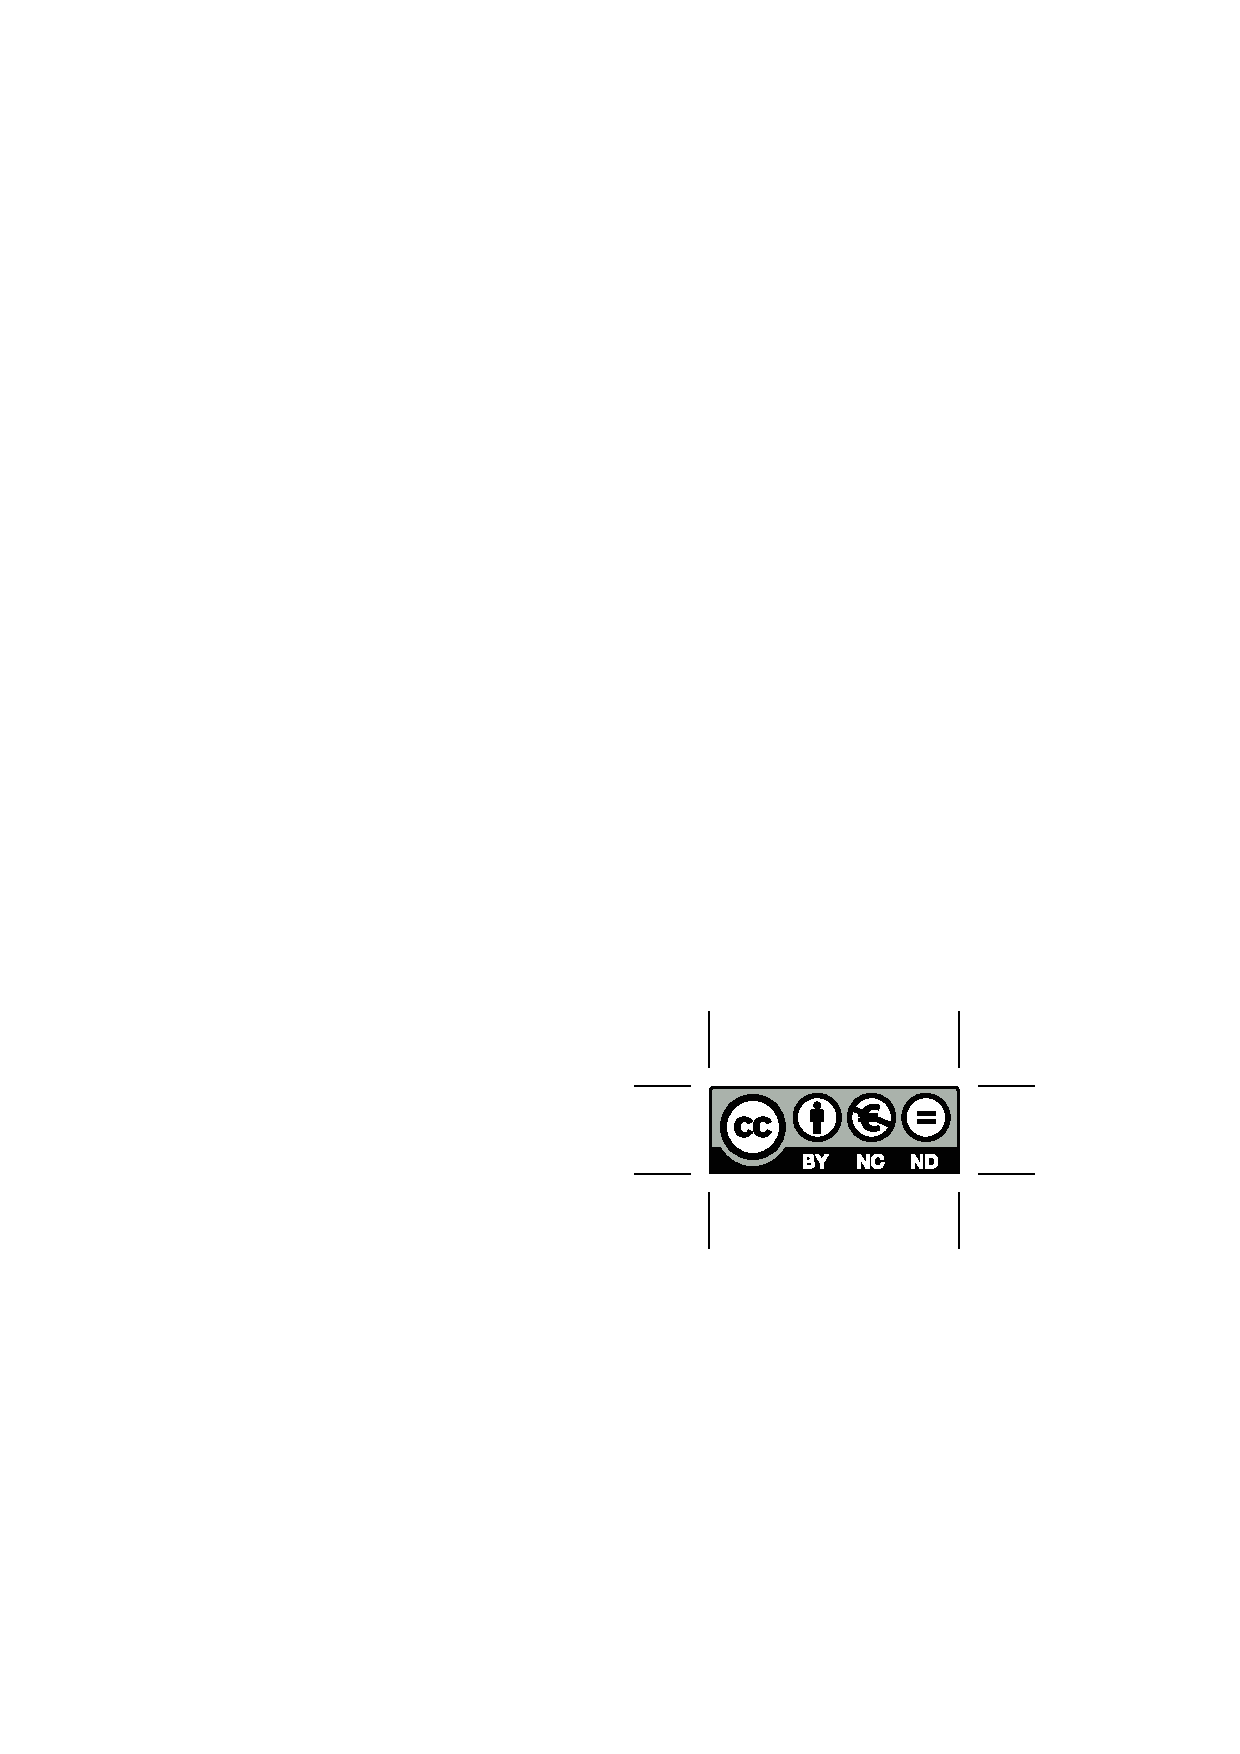
\includegraphics[height=35px]{by-nc-nd-eu}
	\end{minipage}\hfill
\end{center}

Cette \oe{}uvre est mise à disposition selon les termes de la \href{https://creativecommons.org/licenses/by-nc-nd/4.0/deed.fr}{Licence Creative Commons Attribution - Pas d'Utilisation Commerciale - Pas de Modification 4.0 International}. % consultez les conditions de la licence cc by-nc-nd, vous pouvez appliquer une licence moins restrictive, cc by-nc-sa par exemple



	\chapter*{Résumé}					%% résumé
    \addcontentsline{toc}{chapter}{Résumé}
	
\vspace{0.5cm}
Mots clés: cosmologie, énergie noire, spectroscopie



	\chapter*{Abstract}					%% abstract
    \addcontentsline{toc}{chapter}{Abstract}
	%\selectlanguage{english}
	This manuscript summarises my research over the past 12 years in the field of observational cosmology, 
as well as the work by early career scientists for whose I was the main or the co-supervisor.  
The main topic of our work is the study of dark energy with spectroscopic galaxy data 
from the Sloan Digital Sky Survey and the Dark Energy Spectroscopic Instrument. 
We explored three quite different regimes in terms of redshift ranges and types of data:
\lya forests at high-redshift ($2 < z < 3.5$), galaxies at mid-redshift ($0.6 < z < 1.0$)
and type-Ia supernovae at low-redshift ($0 < z < 0.1$). 
We mostly focused on the statistical properties of these samples, estimating two-point functions 
and measuring the scale of baryon acoustic oscillations and the effect of redshift-space distortions. 
We explored new techniques for measuring weak-lensing from \lya forests and the link between galaxies 
and the 21cm radio signal. 
All this research is linked to the challenge of precisely measuring the expansion rate of the 
Universe and the growth-rate of structures, with the hope of finding deviations from 
the standard $\Lambda$CDM cosmological model based on general relativity. 


\vspace{0.5cm}
Keywords: cosmology, dark energy, spectroscopy

	%\selectlanguage{french}


	\chapter*{Acknowledgements}			%% remerciements
    \addcontentsline{toc}{chapter}{Acknowledgements}
	Le modèle de thèse AMU n'existerait pas sans la contribution des doctorants. Nous souhaitons remercier tout particulièrement \href{http://www.theses.fr/2011AIX20720}{Mickaël Bojados}, \href{http://www.theses.fr/2011AIX22111}{Flora Cordoleani} et \href{http://www.theses.fr/2014AIXM4013}{Florian Caullery} pour leur aide précieuse et la qualité de leurs fichiers sources LaTeX. La mise à jour effectuée en 2018 doit beaucoup à l'excellent travail de \href{http://theses.fr/2014ENMP0038}{Dorian Depriester}.

\lipsum[1-2]\index{Nam dui ligula}




    \microtypesetup{protrusion=false}	%% désactive la protrusion (TOC LOFT GLS)
	\tableofcontents					%% TOC
	% \listoffigures						%% LOF
	% \listoftables						%% LOT
	% \printglossary[						%% Acronymes
	% 	type=\acronymtype,
	% 	title={Liste des acronymes},
	% 	toctitle={Liste des acronymes}
	% 	]
	% \printglossary[						%% Glossaire
	% 	title={Glossaire},
	% 	toctitle={Glossaire}
	% 	]
	% \printglossary[						%% Nomenclature
	% 	type=notation,
	% 	title={Nomenclature},
	% 	toctitle={Nomenclature}
	% 	]
    \microtypesetup{protrusion=true}	%% rétabli la protrusion

	\ohead{\leftmark\ifstr{\rightmark}{\leftmark}{}{ -- \rightmark}}	%% place le chapître et la partie en en-tête

	\chapter{Introduction}
	\label{chap:intro}
	%\addcontentsline{toc}{chapter}{Introduction}
	%\localtableofcontents

\vspace{1em}



\section{The history of our Universe and its big open questions}
\label{intro:history_questions}

    Gathering all the knowledge in physics humanity could learn to this day, 
    we are able to come up with a quite interesting and scientifically accurate story,
    describing how our Universe evolved from more than 13.8 billions years ago to nowadays. 
    Our story can explain most of what we observe in the sky, 
    while being consistent with essentially all experimental results obtained on Earth 
    and its Solar neighbourhood.  
    However, the story of our Universe has a few but quite important weak spots. 
    Either because where we do not have 
    a satisfactory physical explanation for some observed phenomena, 
    or simply because some predicted phenomena are not currently observable
    (and potentially will never be).
    That also explain my use of the word \emph{story} instead of \emph{history}, 
    which would only contains verified facts. 

    The story in a nutshell goes as follows: the ``beginning''
    of the Universe\footnote{ The actual beginning of 
    the Universe can be seen as a complex philosophical question or simply as an 
    ill defined physical concept. This discussion is beyond the scope of this work 
    and/or my capabilities. Here, I simply name as ``beginning'' the first epoch of the Universe
    for which we have a widely known physical theory to describe it.}, 
    also known as the \emph{Big Bang} is the start of the \emph{inflation}, 
    an epoch of exponential 
    expansion of space that we believe happened around 13.8 billion years ago. 
    Inflation transformed quantum, microscopic fluctuations of space
    into macroscopic density fluctuations of the Universe's constituents:
    quarks, photons, neutrinos and dark matter. 
    After inflation, the Universe continues to expand but much slowly. 
    The average temperature of the Universe decreases adiabatiacally. 
    Quarks start to gather to form protons, neutrons and relics of heavier atoms, 
    such as deuterium, tritium, helium, lithium and so on. 
    All this during the first few minutes of the Universe's history, in the so called
    \emph{Big Bang nucleosynthesis}. 
    After 380 thousand years, electrons rebind with protons to form neutral 
    hydrogen, while photons scatter for their last time with baryons as the 
    Universe becomes more diffuse. 
    The photons from this epoch are observable today and are known as the 
    \emph{cosmic microwave background}. 
    The Universe then enters its \emph{dark ages}, where hydrogen is mostly neutral and 
    stars have not yet formed. 
    After several million years, gravity clumps hydrogen into dense clouds that reach 
    high enough temperatures to start thermonuclear reactions in their core. 
    The first stars are formed. Then the first galaxies. These galaxies merge into larger 
    galaxies, galaxies form small virialised groups, large groups, clusters, super clusters. 
    Clusters, filamentary structures and voids compose the so called cosmic web. 
    At around half of the Universe's age, the expansion starts to speed up again,
    accelerating, as if gravity became repulsive on very large scales. 
    Then, on one of the many billions of galaxies, the \emph{Milky Way}, 
    planet Earth formed around a somewhat isolated star, the Sun, 
    and here we are today, observing the sky, trying to explain the whole Universe. 

    This story is based on a few assumptions: that general relativity (GR) describes gravity; 
    that the Universe can be modelled as statistically homogeneous and isotropic on large enough
    scales; and that the Universe is composed of the standard model particles and interactions, 
    with the addition of two exotic components: dark energy and dark matter. 

    The origin or nature of the dark sector is one of the biggest mysteries in physics. 
    Several models of dark matter are based on particles beyond the standard model which 
    have not yet been detected, despite the huge experimental efforts towards this goal. 
    The simplest model of dark energy is a cosmological constant which is actually 
    part of GR equations. The possibility that dark energy could be an exotic fluid or 
    the manifestation of an extra force has predicted implications that were not yet 
    observed either. 

    Another weak spot of the story of our Universe is inflation. 
    Up to now, inflation is a successful theory explaining an important set of observations: 
    the homogeneity of the photon temperature 
    from the cosmic microwave background on scales larger than the horizon;
    the flatness of space; and the seeds of structure formation.
    However, the predicted and observable effects of inflation were not yet observed,
    such as primordial gravitational waves.
     
    Solving for the mysteries of the dark sector and inflation 
    would represent major breakthroughs in physics. 
    Large teams of scientists, including myself, are dedicated
    to these puzzles, either theoretically or experimentally. 

    My past work has been focused on observations related to the understanding of dark energy. 
    The rest of this chapter will be dedicated to explaining the problem 
    of accelerated expansion, the dark energy model, alternative solutions,
    and how to observe the expansion. 

\section{Evidences for the accelerated expansion of the Universe}
\label{intro:evidences_acceleration}

    Not long after developing his theory of gravity, Einstein wanted to write a model 
    for a static Universe filled with standard matter. 
    Since gravity is attractive, his solution 
    was to include a new constant term, $\Lambda$, in the equations. 
    This constant, later known as the \emph{cosmological constant}, 
    is one of the simplest models of dark energy, currently
    in agreement with a wide variety of cosmological observations. 
    
    The first indirect evidences for dark energy come from measurements 
    of galaxy clustering in the 1980's 
    (\cite{peeblesTestsCosmologicalModels1984,
    maddoxGalaxyCorrelationsLarge1990, 
    efstathiouCosmologicalConstantCold1990}). 
    At the end of the 1990's, two independent teams measured the expansion of 
    the Universe using type-Ia supernovae as standard candles
    (\cite{riessObservationalEvidenceSupernovae1998, 
    perlmutterMeasurementsOmegaLambda1999}). 
    Their observations could only be explained by 
    an Universe containing around 30 per cent of matter and 70 per cent of dark energy
    in the form of a cosmological constant. 
    Few years later, first measurements of the 
    temperature fluctuations in the cosmic microwave background were consistent with 
    an Universe with a flat space (\cite{balbiConstraintsCosmologicalParameters2000,
    debernardisFlatUniverse2000}), 
    which in combination with measurements of clustering, 
    supernovae and the local expansion rate (\cite{mouldHubbleSpaceTelescope2000}), 
    confirmed the acceleration of our Universe's expansion. 
    Age estimates of globular stellar clusters, which are
    supposed to be among the oldest astrophysical objects, 
    also indicated that the Universe had to be older than the age predicted 
    by models of an Universe only filled with matter (\cite{chaboyerAgeUniverse1998}). 
    The following decade, the 2000's, was enriched with the first measurements
    of the baryon acoustic oscillations in the distribution of galaxies
    (\cite{eisensteinDetectionBaryonAcoustic2005, cole2dFGalaxyRedshift2005}).
    Used as a standard ruler, baryon acoustic oscillations re-confirmed 
    the accelerated nature of the expansion.
    
    Since the 2010's, several cosmological experiments were constructed with the goal of
    improving the precision of all the measurements discussed above. 
    Today, in the 2020's, state-of-the-art measurements of cosmological parameters 
    achieved relative uncertainties of the order of a few percent or less, 
    a quite remarkable score for observational cosmology. 
    Nevertheless, the data shows no evidence for a departure from a model of Universe 
    governed by GR, composed by 70 per cent of this mysterious cosmological 
    constant and 25 per cent by this mysterious dark matter. 

    The future is promising with several stage-IV experiments starting their data taking.
    They will measure millions of galaxy redshifts, billions of galaxy fluxes and shapes, 
    hundreds of thousands of type-Ia supernovae, 
    the cosmic microwave background temperature and polarisation to exquisite 
    precision and resolution, and many more cosmic probes. 
    We truly hope that the data will shed a light over some of the largest mysteries 
    involving our own history. 



\section{Model of an expanding Universe}
\label{intro:model}

    \subsection{Assumptions and ingredients}
    \label{intro:model:ingredients}

    In order to define some important cosmological parameters, I will quickly review
    the basics of the currently most accepted model for our Universe in the limit of 
    very large scales, where it can be considered homogeneous and isotropic. 
    This is also known as the \emph{background} model, since the formation of structures 
    (see next section) can
    be modelled as small perturbations on top of it. 
    It is also assumed that gravity is 
    described by general relativity (GR), which interlinks the fabric of space-time and 
    energy densities of the Universe constituents: 
    \emph{baryons} (protons, electrons, atoms), 
    photons, neutrinos, cold dark matter and dark energy. 

    The expansion of space is usually parametrised by the scale factor $a(t)$, 
    a function of time $t$ that dictates how physical and comoving distances 
    relate to each other. We assume that $a(t_0) = 1$ today ($t_0 = 13.8$ Gyr) 
    and that $a \rightarrow 0$ as $t \rightarrow 0$. The speed of the expansion
    and its acceleration are simply first and second derivatives with 
    respect to time, $\dot{a}(t)$ and $\ddot{a}(t)$, respectively. 
    The expansion rate of the Universe is defined
    as $H(t) = \dot{a}(t)/a(t)$ and takes the Hubble constant value today, 
    $H(t_0) = H_0 = 100 h ~ \mathrm{km/s/Mpc} \sim 70$~km/s/Mpc. 
    Since the scale factor is a monotonically increasing function of time 
    (in our simple model), $a$ is commonly used to describe a given cosmic epoch. 

    One of the consequences of the expansion is that relativistic species, such 
    as photons and massless neutrinos, loose energy or are \emph{redshifted} as they 
    propagate. In astronomy, the redshift $z$ is defined as the relative difference
    in wavelength between the one emitted by source and the one observed.  
    Thus, in an expanding Universe the scale factor is related to the redshift as 
    $a = 1/(1+z)$. Redshift is also commonly used to describe cosmic epoch or distances.
    The time today $t_0$ corresponds to $z=0$ while $z \rightarrow \infty$ as $t \rightarrow 0$. 

    \subsection{The expansion rate}
    \label{intro:model:expansion_rate}

    The expansion rate can be derived from GR equations and be written as a function of 
    redshift and the densities of each constituent
    \begin{equation}
        H^2(z) = H^2_0 \left[ \Omega_m(1+z)^3 + \Omega_r (1+z)^4 + \Omega_\mathrm\mathrm{de}(z) + \Omega_k(1+z)^2\right]
        \label{eq:expansion_rate}
    \end{equation}
    where $\Omega_x = \rho_x / \rho_\mathrm{ crit}$ is the ratio between the density 
    constituent $x$ today and the critical energy density $\rho_\mathrm{ crit} = 3H_0^2/8\pi G$, 
    which is the density required for a flat space geometry. 
    The subscripts $m$, $r$, $de$ and $k$ stand
    for non-relativistic species (baryons, cold dark matter and non-relativistic neutrinos), 
    relativistic species (photons and relativistic neutrinos), dark energy and curvature, 
    respectively. The curvature ``density'' parameter is defined as a function of the others,
    $\Omega_k = (1-\sum_x \Omega_x)$, and it is zero in a flat space geometry.
    Non-relativistic species dilute in an expanding universe so their energy density is 
    proportional to $a^{-3} = (1+z)^3$. Relativistic species dilute as well but have an
    extra factor of $a^{-1}$ due to redshifting. 
    The dark energy term is written as a general function of redshift in Eq.~\ref{eq:expansion_rate}.
    In the simplest case of a cosmological constant, $\Omega_\mathrm\mathrm{de}(z) = \Omega_\Lambda$, i.e. a constant.
    The dependency of curvature with $a^{-2}$ simply comes from the field equations. 

    Figure~\ref{fig:hubble_theory} shows the Hubble expansion rate (times $a(z)$) as a function of redshift $z$
    for a few example of cosmological parameters. All models considered have zero curvature. 
    For all models, the Universe decelerates ($\dot{a}$ decreases) as time goes by (redshift decreases) 
    until dark energy starts to dominate around $z\sim 0.5-0.7$, when the expansion accelerates until today. 
    We can see how the Hubble constant $h$ simply sets the overall amplitude of the curve.
    Also, for increasing values of $\Omega_m$, the transition between matter-dominated to dark energy-dominated era 
    happens at lower redshift. 

    \begin{figure}[t]
        \centering 
        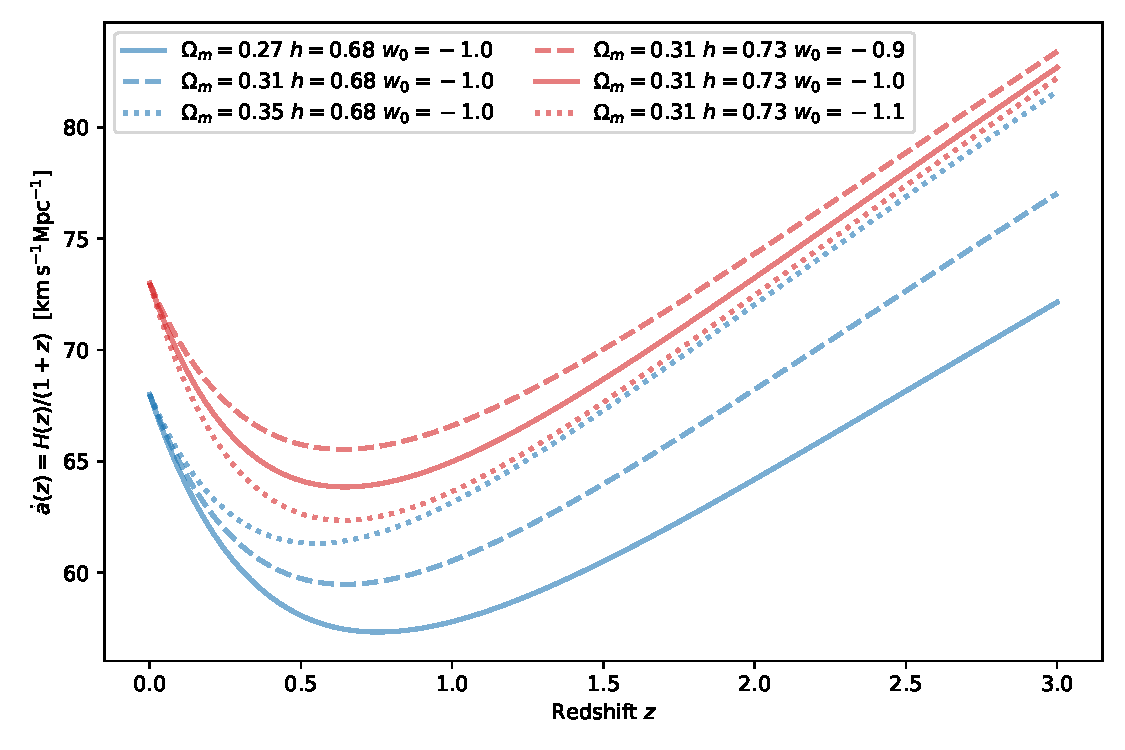
\includegraphics[width=0.9\textwidth]{fig/intro/hubble.pdf}
        \caption{The Hubble expansion rate divided by $(1+z)$, i.e., the speed of expansion $\dot{a}(z)$, 
        versus redshift $z$ for several cosmological models. }
        \label{fig:hubble_theory}
    \end{figure}[t]

    \subsection{Distances in cosmology}
    \label{intro:model:distances}

    Distances are non-trivially defined in an expanding, potentially non-flat, Universe. 
    Therefore, different types of distances are more appropriate for certain observables.
    The \emph{Hubble distance} is related to the expansion rate as 
    \begin{equation}
        D_H(z) = \frac{c}{H(z)},
        \label{eq:hubble_distance}
    \end{equation}
    and it is commonly used in measurements of baryon acoustic oscillations in the line-of-sight 
    direction (see Chapters~\ref{chap:forests} and \ref{chap:galaxies}) or to represent the
    size of a causally connected region (in the future) of the Universe. 
    
    The \emph{comoving distance} to 
    an object at redshift $z$ is written as
    \begin{equation}
        D_C(z)  = \int_0^z \mathrm{d}z' ~ D_H(z').
        \label{eq:comoving_distance}
    \end{equation} 
    This expression yields the distance travelled by a photon from a source towards us but 
    factoring out the scale factor, effectively ``removing'' the effect of expansion. 
    
    The \emph{comoving angular diameter distance} $D_M(z)$ is useful when distances are inferred from 
    angles, which are affected by the curvature of space. 
    An object with comoving size $l$ at a redshift $z$ would be seen with an angular size $\theta$.
    This allows us to define $D_M(z) = l/\theta(z)$ as
    \begin{equation}
        D_M(z)  = D_C(z) \mathrm{sinc} \left(\sqrt{-\Omega_k} \frac{D_C(z)}{D_H(z=0)}\right),
        \label{eq:comoving_ang_diameter_distance}
    \end{equation}
    where $\mathrm{sinc}(x) = \sin(x)/x$. This distance is used in observations of 
    gravitational lensing and in measurements of the baryon acoustic oscillations 
    in the transverse direction to the line-of-sight. 
    
    Analogously, the \emph{luminosity distance} $D_L(z)$ 
    relates the flux $f$ received by an object at redshift $z$ with intrinsic luminosity $L$.
    We define then $D_L(z) = \sqrt{L/4\pi f(z)}$ as
    \begin{equation}
        D_L(z)  = D_M(z) (1+z).
        \label{eq:luminosity_distance}
    \end{equation}
    This distance is used when considering standard candles, where fluxes are used to infer 
    distances. 
    Fluxes of these standard candles vary by several orders of magnitude, 
    so it is handy to define the \emph{distance modulus} as the logarithm of the 
    luminosity distance in units of 10 parsecs (pc):
    \begin{equation}
        \mu(z) = 5\log_{10}\frac{D_L(z)}{10~\mathrm{pc}}.
        \label{eq:distance_modulus}
    \end{equation}
    This definition is such that it easily relates the observed $m(z)$ and absolute $M$ magnitude 
    of an object via $\mu(z) = m(z) - M$.

    In all distances defined above, the dependency to the cosmological energy densities
    $\Omega_x$ happens through $H(z)$ (Eq.~\ref{eq:expansion_rate}). 
    Distance measurements allow us to constrain these parameters. 
    However, all cosmological distance measurements are \emph{relative}, 
    which means they are defined to an arbitrary 
    normalisation\footnote{Two exceptions are parallax distances which are an absolute measurements
    based on the known distance between the Earth and the Sun and gravitational wave distances,
    which amplitudes depend on the distance and on the masses of the progenitors, though
    the masses affect the wave form as well, breaking the degeneracy.}, 
    such as the size of the standard ruler or the intrinsic luminosity of a standard candle.  
    One can ignore this normalisation and still constrain cosmological densities by 
    performing several distance measurements as a function of redshift.
    Or one can use some calibrated estimate of this normalisation, and estimate parameters 
    using a single distance measurement. 
    Note that in all the distances defined above, the dependency with $H_0$ only impacts
    this arbitrary normalisation, so it cannot be measured without assuming 
    the size of the ruler or the luminosity of the candles. 
    It is useful to factor out this dependency with $H_0$, and write distances 
    in units of $h^{-1}$Mpc (numerically equivalent to set $H_0 = 100$~km/s/Mpc). 
    These are the units used in the vast majority of analyses of the large-scale structures 
    and they will be also used throughout this manuscript. 
    
    \subsection{Dark energy models}
    \label{intro:model:dark_energy_models}

    In the Eq.~\ref{eq:expansion_rate} for the expansion rate of the Universe, 
    the dark energy density term is written as a general function of redshift.
    As mentioned before, the simplest model is to consider a cosmological constant
    $\Omega_\mathrm{de}(z) = \Omega_\Lambda$.  
    The cosmological constant can be thought as equivalent to a fluid with 
    negative relativistic pressure $p_\mathrm{de} = -\rho_\mathrm{de}$. 
    This model can be extended by considering a different equation of state 
    $p_\mathrm{de} = p_\mathrm{de}(\rho_\mathrm{de}) = w(z) \rho_\mathrm{de}$, 
    where $w(z)$ can be a constant or a more general function of redshift.
    The only constraint is that $w(z) < -1/3$, which is required to obtain 
    an accelerated expansion in a dark energy dominated Universe. 
    One widely known parametrisation is given by $w(a) = w_0 + w_a(1-a)$ 
    (\cite{chevallierAcceleratingUniversesScaling2001, linderExploringExpansionHistory2003}). 
    
    The literature contains a huge variety of models that attempt to be more physically motivated
    that those just presented (see \cite{weinbergObservationalProbesCosmic2013}, section 2.2 for a review). 
    Some of them suggest that maybe general relativity breaks down on large enough scales, 
    causing the expansion to accelerate. They suggest extensions or modifications to Einstein's 
    theory of general relativity, and are commonly known as \emph{modified gravity} models.   




\section{Model of the large-scale structures}
\label{intro:lss}

    The Universe is clearly not homogeneous and isotropic. 
    Matter clustered under the influence of gravity, creating the cosmic web,
    composed of clusters, filaments, empty regions. 
    The model described in the previous section only describes the Universe
    as a whole, without any inhomogeneities. If we want to describe 
    the evolution of the structures we need to consider an extension to
    the background model. 

    Observations of the large-scale structures and  
    the cosmic microwave background (CMB)
    indicate that the matter density field today is the evolution of 
    tiny density perturbations from the early Universe. 
    Temperature fluctuations in the CMB are of the order of $10^{-5}$, 
    while matter densities today can reach values several orders of magnitude 
    larger than the average density.
    The most widely accepted theory is that the CMB fluctuations,
    and today's structures, are originated
    from the inflation-grown quantum fluctuations, that evolved under the 
    influence of gravity and pressure in the hot dense plasma-like epoch of our Universe. 
    
    It is been possible to model the physics of the evolution of these tiny 
    fluctuations using \emph{linear perturbation theory}. The predictions of this 
    theory are an excellent match to observations of the CMB and to the late-time
    distribution of matter on large scales, i.e., larger than few tens of Mpc. 
    On smaller scales however, gravity becomes highly non-linear and more advanced 
    calculations are required. There are two main approaches to model non-linearities:
    theoretical calculations going beyond linear terms in perturbation theory 
    or numerical n-body simulations. 

    The main idea of perturbation theory is to consider that
    the density of a given species $x$ is given by:
    \begin{equation}
        \rho_x(\vec{x}, t) = \bar{\rho}_x(t)\left[1 + \delta_x(\vec{x}, t)\right],
    \end{equation}
    where the bar indicates average over the whole Universe and 
    $\delta_x \ll 1$ is a small perturbation. The average density 
    $\bar{\rho}_x$ follows the background evolution described in 
    section~\ref{intro:model}. 
    A new set of equations can be derived for the evolution of $\delta_x$ for each species 
    depending if $x$ denotes relativistic species (photons, hot baryons, hot neutrinos) 
    or non-relativistic species (cold baryons, cold neutrinos or dark matter). 
    Only some families of models also consider fluctuations in the dark energy density,
    but most commonly dark energy only acts in the background expansion. 

    The evolution of $\delta_x$ for a given species is dictated by both 
    Boltzmann and Einstein's GR equations. Boltzmann equations describe 
    the evolution of phase-space distributions of each constituent, considering
    collisions (pressure) and particle creation and annihilation. GR equations
    describe how each species influence gravitational potentials which in turn 
    make perturbations grow.

    Another important ingredient in these equations is the 
    \emph{peculiar velocities} $\vec{v}_x(\vec{x}, t)$ of 
    each species, particularly the non-relativistic ones since 
    relativistic species are assumed to have $v \sim c$. 
    Peculiar velocities directly impact the evolution of perturbations through 
    Boltzmann, Euler and continuity equations. 
    These velocities can be measured from galaxies if their distances are estimated.
    They are an important probe of the cosmological model and on the strength of 
    gravity itself. 
    They will be a key actor in chapters~\ref{chap:galaxies} and \ref{chap:velocities},
    where I will discuss redshift-space distortions and the clustering of velocities.  
    
    \subsection{Statistical description of perturbations}
    \label{intro:lss:statistics}

    The value of the matter density field at a given position $\vec{x}$ is 
    hardly observable since most of it is in the form of dark matter. 
    Only baryons which emit photons are observable. 
    Furthermore, it is impossible to learn about the physics of a single value of $\delta_m(\vec{x})$
    since we do not have access to its time evolution: our sky seems static on time-scales 
    of cosmological evolution. 
    
    In order to connect our physical model of structure growth to the observed density field,
    we turn our interest to its statistical properties. We believe that density perturbations 
    are the evolved form of quantum initial perturbations, which would follow Gaussian statistics. 
    If Gaussian, all the information of initial perturbations would be contained in its first two moments.
    The evolution of these perturbations through time modifies these initial statistical properties,
    which become highly complex, for instance creating non-Gaussianities. 
    Therefore, the final density field is described by all higher order moments as well.  

    If we focus on the density field on large scales, most of its cosmological information is
    still contained in the first moments, starting from the
    two-point function (the one-point function is zero by definition),
    which is defined as
    \begin{equation}
        \xi(\vec{x}, \vec{y}) = \langle \delta(\vec{x}) \delta(\vec{y})\rangle 
        \label{eq:two_point_function_config_space}
    \end{equation}
    where $\langle \cdot \rangle$ denotes an ensemble average. Given that
    we only have one single realisation of the Universe, we assume that
    averages over space (in an infinite space) are equivalent to ensemble averages.

    The assumptions of homogeneity and isotropy of the background can be 
    applied in an statistical sense to the perturbations. Statistical 
    homogeneity makes $\xi$ not to depend on the specific locations $\vec{x}$
    and $\vec{y}$ but only on their separation $\vec{r} = \vec{y}-\vec{x}$. 
    Statistical isotropic makes $\xi$ no longer depend on the orientation of
    $\vec{r}$, only on its absolute value $r = |\vec{r}|$. 
    Therefore, the two-point correlation function simplifies to a function of $r$:
    \begin{equation}
        \xi(r) = \langle \delta(\vec{x}) \delta(\vec{x}+\vec{r})\rangle. 
        \label{eq:two_point_function_config_space_iso_homo}
    \end{equation}
    
    The correlation function $\xi(r)$ is a powerful observable which can 
    be compared to predictions from a given cosmological model. 
    Most of my work was dedicated to measuring correlations with galaxy survey data. 

    
    \subsection{Configuration and Fourier space}
    \label{intro:lss:config_fourier}

    The time evolution of linear density perturbations $\delta(\vec{x})$ 
    is dictated by a set of second-order differential equations, containing 
    derivatives with respect to time and space. 
    It is thus convenient to apply Fourier
    transforms to these equations, where derivatives with respect to space 
    become simple products. Separations $\vec{r}$ in the so-called 
    \emph{Configuration space} become wavevectors $\vec{k}$ in 
    \emph{Fourier space}. The density perturbations in Fourier space are
    defined by 
    \begin{equation}
        \tilde{\delta}(\vec{k}) = \int \mathrm{d}^3x \ \mathrm{e}^{- i \vec{k}\cdot\vec{x}} \delta(\vec{x}),
    \end{equation}
    and its inverse is
    \begin{equation}
        \delta(\vec{x}) = \frac{1}{(2\pi)^3}\int \mathrm{d}^3k \ \mathrm{e}^{+i \vec{k}\cdot\vec{x}} \tilde\delta(\vec{k}),
    \end{equation}
    where integrals are assumed to be performed over an infinite volume. 

    As previously, we are interested in the two (or more) point functions of the
    field. In Fourier space, the two-point correlation function is known as the
    \emph{power spectrum} and is defined as
    \begin{equation}
        \left\langle \tilde\delta(\vec{k}) \tilde\delta(\vec{k})' \right\rangle = (2\pi)^3 P(k) \delta^3_\mathrm{Dirac}(\vec{k}-\vec{k}'),
        \label{eq:power_spectrum_definition}
    \end{equation}
    where $\delta^3_\mathrm{Dirac}(\vec{x})$ is a three-dimensional Dirac distribution.
    The assumption of spatial homogeneity is guaranteed by the properties of Fourier space,
    while the assumption of isotropy makes the power spectrum to be only a function of the
    absolute value of the wavevector $k = |\vec{k}|$. 

    When considering the evolution of perturbations in Fourier space to the linear level,
    each mode $\tilde\delta(\vec{k})$ evolves independently of the others. We often say 
    that there is no \emph{mode coupling} in linear theory. 

    The power spectrum $P(k)$ is an observable, as powerful as the correlation function,
    to constrain cosmological models. While in theory these two contain exactly the
    same compressed statistical information, in practice the analyses of real data  
    use different finite ranges of scales which are affected differently by systematic effects. 
    Therefore, analyses of real data in configuration and Fourier space complement each other. 
    My contributions to such analyses are presented in chapter~\ref{chap:galaxies}. 

    \subsection{Cosmological dependency of the power spectrum}
    \label{intro:lss:cosmology_dependency}

    The power spectrum $P(k)$ or the correlation function $\xi(r)$ of density 
    perturbations are excellent probes of the cosmological model. 
    They encode information accumulated over the whole Universe's history, 
    since the Big Bang until today.

    At the end of inflation, we think that perturbations were roughly Gaussian 
    (as are quantum fluctuations of the vacuum), 
    having a nearly scale independent power spectrum defined by
    \begin{equation}
        P_0(k) = A_s k^{n_s-1},
        \label{eq:initial_power_spectrum}
    \end{equation}
    where $A_s \sim 2 \times 10^{-9}$ is the amplitude of scalar perturbations 
    and $n_s \sim 0.96$ is the scalar spectral index. The term scalar refers to 
    standard density (or gravitational potential) perturbations, 
    while tensorial perturbations (of the space-time metric) refer to 
    primordial gravitational waves. Vectorial perturbations decay and rapidly become
    negligible in most common cosmological models. 

    After inflation, the majority of the energetic budget of Universe was held
    by relativistic species: photons and neutrinos. Since their energy density decays as $a^{-4}$, 
    their contribution quickly drops. This radiation-dominated era lasted until 
    $z \sim 5000$, or $t \sim 20$~kyr, when the energy density of matter became 
    the dominant source. Matter density decays at a slower rate, proportional to $a^{-3}$.
    dark energy became dominant at $z \sim 0.5$, or $t \sim 9$~Gyr, since its 
    energy density is constant (or close to constant).  
    The actual duration of each era depends on relative values of 
    the energy densities, parametrised by $\Omega_x$ 
    (see \ref{intro:model:expansion_rate}). 

    Matter perturbations grew at different rates during these different eras.
    Figure~\ref{fig:pk_evolution} shows how the power spectrum grows over time 
    for different species and for different scales. 
    In radiation-dominated era, large-scale modes (large values of $r$ 
    or small values of $k$) grew while small-scale ones oscillated,
    due to battle between gravity and radiative pressure. 
    These are known as \emph{baryon acoustic oscillations}. These oscillations
    are imprinted in the power spectrum of the photon-baryon fluid, at the time of the CMB, 
    and in the matter power spectrum at later times. 
    The radiative pressure prohibited the growth of small-scale perturbations,
    so the matter power spectrum is damped, which results in this hill-like shape. 
    In the matter-dominated era, the radiative pressure becomes negligible 
    and all modes grow equally (neglecting non-linear growth). 
    When dark energy is dominant, the expansion accelerates and 
    growth of structures slows down slightly. 
    
    \begin{figure}[t]
        \centering
        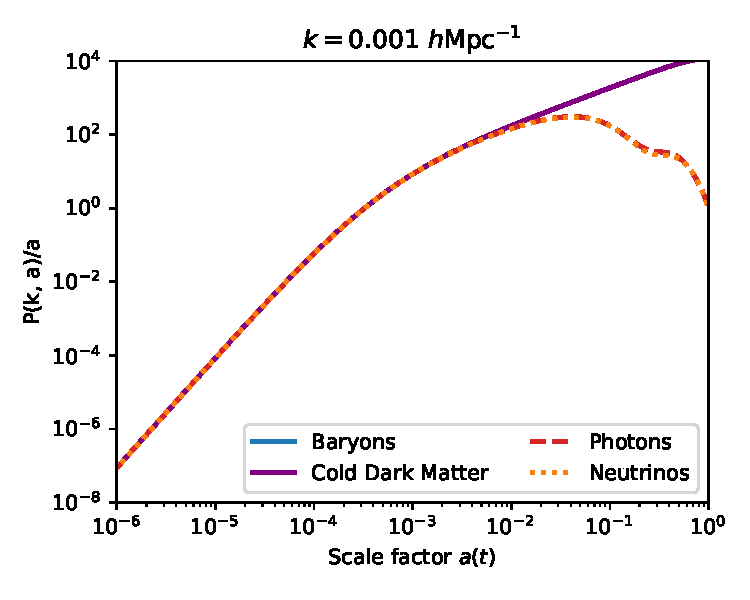
\includegraphics[width=0.49\textwidth]{fig/intro/pk_versus_time_k0.001.pdf}
        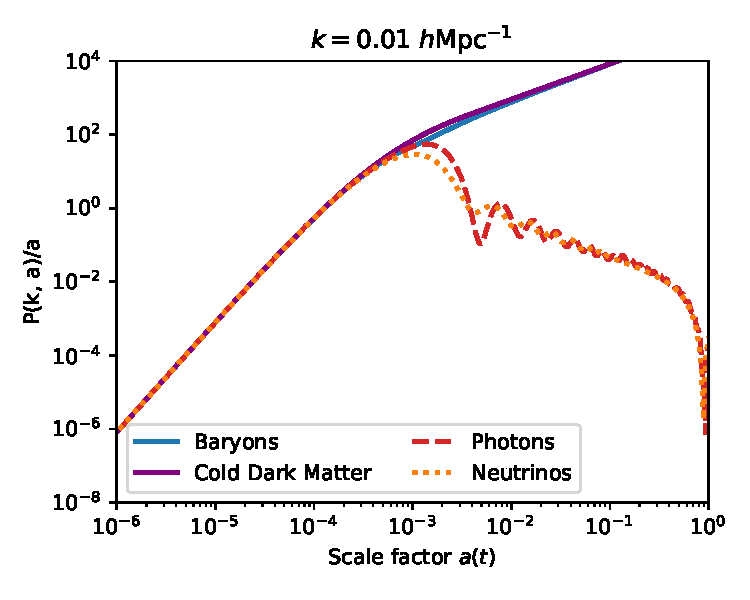
\includegraphics[width=0.49\textwidth]{fig/intro/pk_versus_time_k0.01.pdf}
        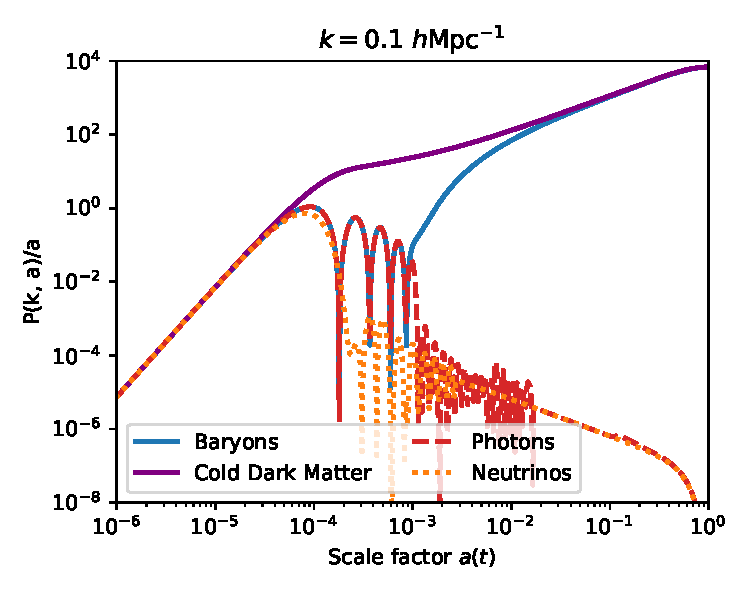
\includegraphics[width=0.49\textwidth]{fig/intro/pk_versus_time_k0.1.pdf}
        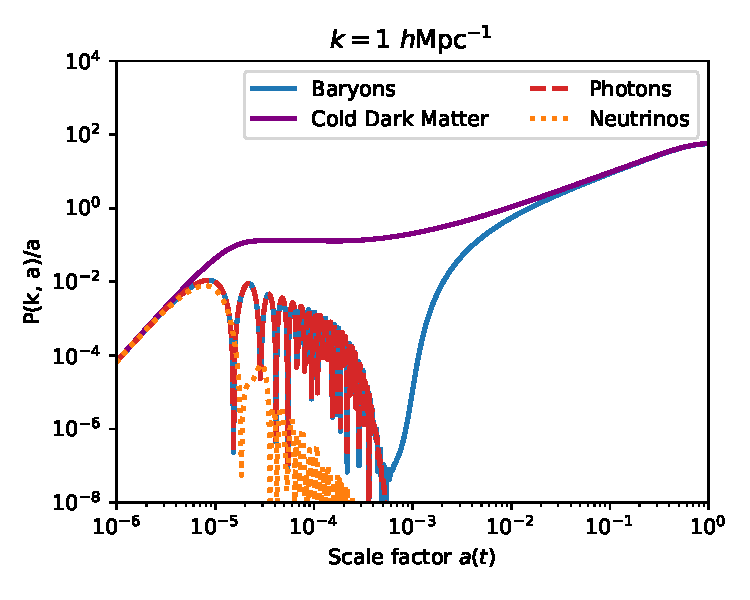
\includegraphics[width=0.49\textwidth]{fig/intro/pk_versus_time_k1.pdf}
        \caption{Evolution of the amplitude of the power spectrum versus the scale factor 
        for four different species and four different scales (one per panel). 
        The evolution was computed using \textsc{CAMB}. A movie version can be found 
        at \url{https://github.com/julianbautista/movie_correlations}.}
        \label{fig:pk_evolution}
    \end{figure}[t]

    Well after recombination,
    matter (baryons + dark) density perturbations obey the following differential equation, if we 
    assume GR and linear theory:
    \begin{equation}
        \ddot\delta(\vec{x}, t) + 2H(z)\dot\delta(\vec{x}, t) - \frac{3}{2} \Omega_m H_0^2 (1+z)^3 \delta(\vec{x}, t) = 0. 
        \label{eq:growth_equation}
    \end{equation}

    If we assume that $\delta(\vec{x}, t) = \delta(\vec{x}, t_0) G(t)/G(t_0)$, we can factor out 
    the spatial dependency and only solve for the time-dependent term $G(t)$, known as the 
    \emph{growth factor}. Its logarithmic derivative with respect to the scale factor $a(t)$ 
    is called \emph{growth rate} of structures:
    \begin{equation}
        f(a) \equiv \frac{ \mathrm{d}~ \ln G(a)}{\mathrm{d}~ \ln a},
        \label{eq:growth_rate}
    \end{equation}
    which is a key observable for which the predicted value 
    depends on the cosmological parameters and on the assumed
    theory of gravity (e.g., GR in Eq.~\ref{eq:growth_equation}). 

    In linear theory, the peculiar velocity field is simply related to 
    density perturbations via the continuity equation 
    \begin{equation}
        \nabla \cdot \vec{v}(\vec{x}, a) 
            \equiv \theta(\vec{x}, a) 
            = -a^2 H(a) \frac{\mathrm{d}\delta(\vec{x}, a)}{\mathrm{d}a} 
            = -a H(a) f(a) \delta(\vec{x}, a) 
        \label{eq:velocity_from_density}
    \end{equation}
    where $\theta$ is the velocity divergence, a convenient scalar field describing velocities. 
    In Fourier space, the velocity field is simply proportional to the density. 
    The velocity divergence power spectrum $P_{\theta \theta}$ is an important ingredient 
    for models of redshift-space distortions, as we discuss in the following section. 

    \subsection{The amplitude of the power spectrum}
    \label{intro:lss:amplitude_power_spectrum} 
    
    The matter power spectrum $P(k)$ represents the variance of density perturbations 
    at a given wavenumber $k$. The total variance of the density field is therefore 
    the sum of all contributions over all available three dimensional modes. 
    This is equivalent to the correlation function at zero separation:
    \begin{equation}
        \sigma^2 = \xi(r=0) = \frac{1}{(2\pi)^3}\int \mathrm{d}^3k ~ P(k) = \frac{1}{2\pi^2} \int_0^\infty \mathrm{d}k ~k^2 P(k), 
        \label{eq:variance_linear_field}
    \end{equation} 
    which diverges if we use the linear prediction for the matter power spectrum.
    This is because the linear power spectrum is the evolution of a nearly scale 
    invariant power spectrum, equivalent to white noise, so the variance simply 
    keeps increasing as we consider larger ranges of scales. Therefore, it is 
    convenient to smooth the linear density field using a three-dimensional 
    top-hat filter with radius $R$. The variance of the smoothed field is 
    then 
    \begin{equation}
        \sigma_R^2 = \frac{1}{2\pi^2} \int_0^\infty \mathrm{d}k ~k^2 P(k) W_R^2(k),
        \label{eq:variance_linear_field_smoothed}
    \end{equation}
    where $W_R(k) = 3[\sin(kR) - kR \cos(kR)]/(kR)^3$ is the Fourier transform of the
    top-hat filter in three dimensions. 

    In studies of large-scales structures, it is common to use $\sigma_R^2$ 
    as a parameter defining the amplitude of the linear power spectrum. 
    As discussed before, this amplitude depends on the values of $A_s$ (Eq.~\ref{eq:initial_power_spectrum})
    and $h$, which determines the age of the Universe and how long structures could have grown.
    Therefore $\sigma_R^2$ is degenerate with $A_s$ and $h$ though is more representative of
    the amplitude of $P(k)$ at later times.  
    Other energy density parameters $\Omega_x$ also affect this amplitude, but these
    also change the overall shape and are not degenerate with $\sigma_R$. 

    The variance $\sigma_R$ is a decreasing function of $R$. Historically, 
    the chosen values for $R$ yield variances near unity, which correspond to 
    the regime where linear theory should break.   
    Recently, the value of $R = 8h^{-1}$Mpc has been used in several analysis, 
    though it has been argued that choosing $R = 12$~Mpc (without the $h$ dependency)
    is a better choice to break degeneracies (\cite{sanchezArgumentsUsingMpc2020}).
    The accepted value for $\sigma_8$ is around 0.8. 

    In measurements of redshift-space distortions and peculiar velocities, 
    there is a degeneracy between the value of $f$ and the
    amplitude of the power spectrum, $\sigma_8$. Therefore, 
    measurements can only constrain the combination $f\sigma_8$
    (see more in chapter~\ref{chap:galaxies}).


    

\section{Cosmological probes of expansion}
\label{intro:probes}

    In this section, I present the basics of the cosmological 
    observables that allow us to learn about dark energy. 
    Some of these are mostly sensitive to the background evolution
    presented in section~\ref{intro:model:expansion_rate}, while others 
    depend on the matter perturbations and their statistical properties as 
    discussed in section~\ref{intro:lss}. 

    \subsection{Direct measurements of \texorpdfstring{$H_0$}{the Hubble constant}}
    \label{intro:probes:h0}

    The Hubble constant $H_0$ is probably one of the first cosmological parameters 
    to be estimated by the person giving its name to it (\cite{hubbleRelationDistanceRadial1929}).
    Today, there are a few techniques to estimate $H_0$ which yield roughly independent results.
    See \cite{riessExpansionUniverseFaster2020} for a quick review of the latest results.  

    The most traditional method is known as the \emph{distance ladder}. 
    The idea is to measure the distance-redshift relationship of objects 
    well in the Hubble flow, i.e., far enough so they feeling the expansion. 
    The distance to the closest objects in the Solar neighbourhood can 
    be estimated with the parallax method. The Gaia satellite has the current largest catalogue 
    of parallax measurements, containing more than a billion stars. 
    Parallax is one of the few direct distance estimating methods. They can be used to 
    measure the intrinsic luminosity of some objects thought to be standard candles, such as 
    Cepheid stars, RR Lyrae, and the largest red giant stars. 
    One can use these candles to estimate distances to even more distant objects, 
    explaining the usage of the word \emph{ladder}. 
    \cite{riessCosmicDistancesCalibrated2021a} contains the latest measurements using 
    Gaia parallaxes, Cepheids and type-Ia supernovae 
    to determine $H_0 = 73.0 \pm 1.4$~km/s/Mpc.  
    \cite{freedmanCarnegieChicagoHubbleProgram2019}
    is latest measurement of distances using the tip of the red giant branch. 
    
    The distance to the galaxy NGC 4258 could be determined thanks to the presence of a 
    water maser orbiting the center of this galaxy. The proper motions of several
    clouds orbiting close to the central massive black hole could be measured both 
    in radial and angular directions, strongly constraining the dynamics of the system
    (\cite{herrnsteinGeometricDistanceGalaxy1999b}).
    The most recent measurement yields $D = 7.576\pm0.082$~(stat.)~$\pm0.076$~(sys.)~Mpc
    (\cite{reidImprovedDistanceNGC2019}), which can be used as an alternative
    to Cepheids to anchor the 
    distance ladder and provide an estimate to $H_0$. 


    Another alternative method is based on the time-delay of the signals emitted from 
    a quasar behind a strong gravitational lens. The lens creates multiple images of the
    same background quasar, but the light paths have slightly different lengths. 
    Since quasars are variable objects, the same variability is observed with a delay of 
    several days between the different images. 
    By modelling the distribution of matter between the quasar and us, 
    it is possible to convert these time delays into an estimate of $H_0$.
    The collaboration named ``$H_0$ Lenses in COSMOGRAIL's Wellspring'', or \textsc{H0LiCOW}, 
    produced the latest comprehensive measurement of $H_0$ using strongly-lensed quasars
    (\cite{wongH0LiCOWXIIICent2019}). 
    An alternative measurement has been performed using strong lenses from the Sloan (SLACS). 
    They are compared to \textsc{H0LiCOW} in \cite{birrerTDCOSMOIVHierarchical2020}. 
    
    More recently, gravitational waves from a merger of two black holes were 
    observed for the first time by the LIGO collaboration
    (\cite{theligoscientificcollaborationObservationGravitationalWaves2016}). 
    Not long after, a merger of two neutron stars was observed by both LIGO and Virgo,
    but this time an electromagnetic counterpart was also detected
    (\cite{theligoscientificcollaborationGW170817ObservationGravitational2017}), 
    pointing to the galaxy where the event occurred. Given the well predicted 
    shape of the wave form and its dependency on the masses of the neutron stars,
    it was possible to estimate the luminosity distance to the host galaxy independently of its redshift. 
    By combining this distance with an actual measurement of the host galaxy redshift, 
    a single event could provide a rough estimate of $H_0$ 
    (\cite{abbottGravitationalwaveStandardSiren2017b}). 
    This measurement opened the field of cosmology using standard sirens, i.e., gravitational wave sources. 

    The cosmic microwave background can yield an estimate of 
    $H_0$ but it is strongly degenerate with other unknown parameters, such as curvature
    or dark energy densities. Some of these degeneracies are reduced when considering 
    the effect of gravitational lensing of the CMB or when combining with other probes
    of late times. Therefore, precise measurements of $H_0$ from the CMB alone are only 
    possible when considering more restrictive models, such as a flat 
    space with a cosmological constant. 

    \subsection{Type-Ia supernovae}
    \label{intro:probes:snia}

    As mentioned earlier, type-Ia supernovae (SNIa) can be used as standard candles for 
    absolute distance measurements, if they are anchored by another method. 
    The SNIa can also be used without anchors to produce relative distance measurements and 
    constrain dark energy. In this case, the only assumption is
    that the SNIa intrinsic brightness does not evolve with redshift. 
     
    The main observable are the fluxes of SNIa as a function of time in different 
    photometric bands, known as light-curves. Spectroscopic follow up observations of 
    the explosion can confirm the type of the supernova based on the features
    present in their spectra. Another key ingredient is the redshift of the host 
    galaxy of the SNIa, which is commonly measured with spectroscopy as well.
    
    Spectro-photometric models of SNIa are used to fit the observed 
    light-curves, yielding their apparent magnitudes 
    at peak luminosity in a given photometric band. 
    These models account for correlations between colour and duration of light curves 
    and the peak magnitude, reducing the intrinsic scatter in these magnitudes from 
    40\% to roughly 15\%. 
    It is essential to obtain accurate and precise measurements 
    of SNIa fluxes in order to obtain the best cosmological constraints. 
    Large sets of realistic simulations of the data are required in order to 
    correct for selection effects. The final product of the analysis is a set
    of distance moduli (Eq.~\ref{eq:distance_modulus}) and their host-galaxy redshift, 
    which can then be compared to models of expansion of the Universe. 
    
    Distance moduli depend on dark energy through the integral of $H^{-1}(z)$ 
    (Eq.~\ref{eq:luminosity_distance} and \ref{eq:distance_modulus}). 
    In order to obtain good constraints on dark energy properties, it is 
    important to have a large redshift coverage, at least covering the 
    transition between matter-dominated to dark energy-dominated eras, so over 
    $0< z< 1$. The advantage of SNIa for dark energy studies is that they 
    can span these redshifts with a high sampling rate, which helps in 
    the study of the expansion rate. One of the inconveniences is that SNIa 
    are complex and poorly understood astrophysical events, the intrinsic 
    scatter in luminosity cannot be reduced to better than 12\%, potentially 
    limiting the gains constraining power from future experiments. 
     
    The latest comprehensive study of SNIa combines data from more than a dozen 
    projects into a single sample, the Pantheon sample, from which dark energy 
    constraints were derived (\cite{scolnicCompleteLightcurveSample2018}).
    The Dark Energy Survey also measured a more recent sample of few hundreds of SNe
    (\cite{broutFirstCosmologyResults2019a, broutFirstCosmologyResults2019, 
    kesslerFirstCosmologyResults2019}), 
    but not all  have spectroscopic classification. 
    Their constraints on dark energy are not yet competitive compared to the Pantheon sample. 
    The Zwicky Transient Facility (ZTF, \cite{grahamZwickyTransientFacility2019}) 
    is currently observing the Northern sky 
    on a search for transient events and is expected to discover around 5000 
    spectroscopically confirmed SNIa at low redshifts ($0< z< 0.12$) until 2023. 
    After 2023, the Rubin Observatory Legacy Survey of Space and Time (LSST) 
    will take over in the Southern hemisphere
    and will discover more than 300 thousand SNIa up to $z< 0.5$. 
    
    While ZTF and Rubin's samples of SNIa will not decrease significantly the 
    errors on dark energy parameters, they cover a redshift range where other 
    powerful probes, such as baryon acoustic oscillations or weak-lensing, 
    lack of statistical power due to limited volume. 
    Furthermore, at lower redshifts when dark energy is dominant, SNIa are 
    complementary to redshift-space distortions (RSD) when it comes to testing 
    the validity of GR or constraining alternative models of gravity,
    as solutions for dark energy. 

    Not only SNIa are a great probe of the 
    expansion history, they can also provide peculiar velocities of their 
    host galaxies via their inferred distances. 
    These peculiar velocities and their statistical properties can complement 
    RSD analysis when measuring the growth-rate of structures 
    (Eq.~\ref{eq:growth_rate}). Estimates of $H(z)$ and $f(z)$ can help 
    break degeneracies between simple dark energy models and more involved 
    models of gravity (\cite{kimComplementarityPeculiarVelocity2020, 
    grazianiPeculiarVelocityCosmology2020}). 
    Chapter~\ref{chap:velocities} is dedicated to this 
    topic, to which I plan to dedicate the next few years of my research.  


    \subsection{Big Bang nucleosynthesis}
    \label{intro:probes:bbn}

    In the post-inflation Universe, when temperatures
    are below the equivalent of 100 MeV, perturbations in the
    matter and radiation fields are quite 
    small and most of the physics is dictated by the interactions 
    between protons, electrons, neutrons, and photons,
    as described by the Boltzmann equations. 
    As the Universe cools down and rarefies, protons and neutrons 
    start forming atoms of deuterium, tritium, helium and heavier elements.
    This process is known as the Big Bang nucleosynthesis (BBN).

    The relative amount of each of the formed elements depends on the expansion rate 
    of the Universe at that time as well as the physical density of baryons 
    $\omega_b = \Omega_b h^2$ and radiation $\omega_r = \Omega_r h^2$.
    Given that the energies involved are within reach of particle 
    accelerators, these reactions can be studied with great detail on Earth,
    allowing us to build accurate models of the BBN 
    (see \cite{pitrouNewTensionCosmological2021} for the latest calculations
    and references therein). 
    
    Observations of the primordial abundances can be compared to the predictions 
    by BBN models. Abundances of deuterium, helium, and others can be estimated 
    from spectroscopic observations of HII regions in metal-poor galaxies 
    or from absorption lines of the intergalactic medium in quasar spectra. 
    The most up-to-date measurements of the primordial helium-4 abundance yields 
    $Y_p = 0.2453 \pm 0.0034$ (\cite{averImprovingHeliumAbundance2021}), while
    the deuterium one is $\mathrm{D/H} = (2.527 \pm 0.030) \times 10^{-5}$
    (\cite{pitrouNewTensionCosmological2021}). 
    While observations are consistent with BBN models for deuterium and helium, 
    the abundance of lithum-7 exhibits a factor 3 discrepancy, which is a huge problem 
    in BBN but quite often neglected. 
    
    The temperature fluctuations in the cosmic microwave background (CMB) are
    also very sensitive to the physical baryon density $\omega_b$. 
    Historically, the values obtained from CMB have been in good agreement 
    with BBN measurements, showing that baryons make up to around 16\% of the total 
    matter content of the Universe, or $\omega_b = (2.195 \pm  0.022)\times 10^{-2}$. 
    The agreement between two quite independent probes is one of the great successes 
    of the current cosmological model, thought they also enforce the need for a dark matter 
    component.  

   
    \subsection{Baryon acoustic oscillations}
    \label{intro:probes:bao}

    Baryon acoustic oscillations (BAO) is the name given to the propagation of sound
    waves in the primordial plasma (baryons and photons), prior to recombination. 
    Because of the high pressure on small scales at those times, 
    each initial density perturbation had a spherical density wave around them 
    propagating outwards at the speed of sound in that medium. The speed of sound
    in the plasma is given by 
    \begin{equation}
        c_s(z) \equiv \sqrt{\frac{1}{3[1+R(z)]}}
        \label{eq:sound_speed}
    \end{equation}
    where $R(z) = 3\rho_b / 4 \rho_\gamma$ is the baryon-to-photon ratio.
    The propagation of sound waves occurred until the temperatures and densities 
    dropped to values such that baryons no longer 
    felt the pressure from photons, known as the \emph{drag epoch}, which is 
    close in time to the recombination (but technically not the same epoch), at $z\sim 1100$. 
    This process left a slight over dense shell of matter around each initial perturbation
    with a radius given by 
    \begin{equation}
        r_\mathrm{drag} \equiv r_s(z_\mathrm{drag}) = 
            \int_\infty^{z_\mathrm{drag}} \mathrm{d}z' \frac{c_s(z')}{H(z')}
        \label{eq:sound_horizon}
    \end{equation}
    which is known as the \emph{sound horizon at drag epoch}, or the BAO scale. 
    Today, $r_d$ has a physical size of about 147 Mpc, much larger than any 
    collapsed structure in the Universe. 
    As one can see from Eqs.~\ref{eq:sound_speed}
    and \ref{eq:sound_horizon}, $r_\mathrm{drag}$ mainly depends on 
    $\omega_b$ and $\omega_c$ assuming the CMB gives a precise 
    estimate of $\omega_\gamma$. The dependency of $r_\mathrm{drag}$ 
    is mainly through $\omega_b$.

    After recombination, the sound horizon scale only increases in size 
    due to the expansion, or equivalently, its comoving size remains unchanged. 
    Therefore, the BAO scale is a great \emph{standard ruler} to study the expansion 
    rate of the Universe. 
    In practice, the BAO scale is observed statistically in the 
    two-point function of the matter density field, so it is often 
    classified as an statistical standard ruler. 
    In configuration space, the correlation function $\xi(r)$ presents a small 
    peak at separations corresponding to the BAO scale $r_d$, while in Fourier space 
    the power spectrum $P(k)$ contains an oscillatory pattern as a function of scale 
    with a period proportional to the BAO scale.  
    In chapters~\ref{chap:forests} and \ref{chap:galaxies}, I present 
    my past work in the measurement of the BAO scale using \lya\ forests 
    and galaxies, respectively, as tracers of the matter density field.
    
    Given that a galaxy survey is made of angular positions and redshifts, 
    which are true observables, 
    the BAO peak is effectively measured as an angle $\Delta \theta_\mathrm{BAO}$ 
    or as a difference in redshift $\Delta z_\mathrm{BAO}$. 
    These can be modelled as ratios of distances to the BAO scale $r_d$ as
    \begin{equation}
        \Delta \theta_\mathrm{BAO}(z_\mathrm{eff}) = \frac{D_M(z_\mathrm{eff})}{r_d}
        \label{eq:bao_angular}
    \end{equation}
    \begin{equation}
        \Delta z_\mathrm{BAO}(z_\mathrm{eff}) = \frac{D_H(z_\mathrm{eff})}{r_d}
        \label{eq:bao_radial}
    \end{equation}
    where $z_\mathrm{eff}$ is the effective redshift of the galaxy survey, 
    $D_M$ is the comoving angular diameter distance (Eq.~\ref{eq:comoving_ang_diameter_distance}),
    and $D_H$ is the Hubble distance (Eq.~\ref{eq:hubble_distance}). 

    There are two ways BAO can be used to constrain cosmological models, 
    depending if we assume that $r_\mathrm{drag}$ is known or not. 
    If $r_\mathrm{drag}$ is known, i.e. given by Eq.~\ref{eq:sound_horizon} 
    using some value for $\omega_b$
    (given by the CMB or BBN for instance), then BAO measurements
    are converted to absolute distance measurements which depend only on  
    $H(z)$. Therefore, BAO can constrain $H_0$, curvature and dark energy. 
    If $r_\mathrm{drag}$ is supposed to be unknown but still a standard ruler, 
    then BAO constraints the ratio of $E(z) = H(z)/H_0$ to the combination 
    $H_0 r_\mathrm{drag}$ which is now degenerate. This is similar to the case of
    type Ia supernovae, where their absolute magnitude is degenerate with $H_0$.
    By combining several BAO measurements at different effective redshifts, 
    BAO is a powerful probe of dark energy and curvature. 

    Current BAO measurements span effective redshifts from 0.1 to 2.3.
    The Sloan Digital Sky Survey (SDSS, 
    \cite{eisensteinSDSSIIIMassiveSpectroscopic2011, blantonSloanDigitalSky2017}) 
    has measured more than 2 million 
    redshifts spectroscopically in the past twenty years, 
    producing the largest maps to date of the
    distribution of matter in the Universe. In addition to SDSS, 
    surveys such as FastSound (\cite{okumuraSubaruFMOSGalaxy2016}), 
    Vipers (\cite{pezzottaVIMOSPublicExtragalactic2017}),
    6 degree field galaxy survey (6dFGS, \cite{beutler6dFGalaxySurvey2012a})
    and WiggleZ (\cite{parkinsonWiggleZDarkEnergy2012}) also
    produced BAO measurements using galaxies, though the volumes 
    probed and the number of galaxies is inferior to SDSS. 
    The latest cosmological constraints from BAO are described in 
    \cite{alamCompletedSDSSIVExtended2021}.



    \subsection{The cosmic microwave background}
    \label{intro:probes:cmb}

    The cosmic microwave background (CMB) is one of the richest cosmological probes of all. 
    The photons we receive today last scattered on baryons at a redshift of about 1100,
    corresponding to roughly 380 000 years after the Big Bang. 
    It is currently the oldest information that we can measure from the Universe today. 
    
    The average temperature $T_\mathrm{CMB} = 2.72548 \pm 0.00057$~K 
    (\cite{matherMeasurementCosmicMicrowave1994, fixsenTemperatureCosmicMicrowave2009}) 
    of these photons, measured by the COBE satellite, tell us on how much 
    energy density from radiation there is in the Universe. 
    Considering a black body Bose-Einstein distribution for the photons, we have that 
    \begin{equation}
        \rho_\gamma = \frac{\pi^2 k^4}{15 \hbar^3 c^3} T_\mathrm{CMB}^4
        \label{eq:energy_density_photons}
    \end{equation} 
    
    The fluctuations around this average temperature, $\Delta T$, 
    and the polarisation of these photons
    trace the structures back at the recombination epoch. 
    Given its early-times nature, 
    the temperature and polarisation fields are extremely well described by 
    Gaussian statistics. Most of the information is therefore contained in the two point
    functions of these fields. Given that these fields are functions of
    the position angle in the sky $(\theta, \phi)$, it is convenient to decompose these 
    fields into a basis of spherical harmonics $Y_{\ell m}(\theta, \phi)$.
    The amplitude of each harmonic is denoted $a_{\ell m}$. The angular power spectrum  
    is simply the variance of these amplitudes: $C_\ell = \langle a_{\ell m} a^*_{\ell m}\rangle$, 
    which in linear theory is simply a function of $\ell$ and independent of $m$. 
    The temperature and both E and B polarisation modes of the CMB can be decomposed into 
    spherical harmonics, so we can estimate all cross power spectra, e.g., 
    $C^{TE}_\ell = \langle a^T_{\ell m} a^{E*}_{\ell m}\rangle$ is the
    cross temperature and E-mode polarisation power spectrum. 
    
    The temperature and polarisation auto and cross power spectra 
    are exquisitely well modelled by linear perturbation theory. 
    In the most basic $\Lambda$CDM model, the power spectrum is a 
    function of only six parameters: the angular scale of baryon 
    acoustic oscillations $\theta_*$, 
    the physical density of baryons $\omega_b$ and dark matter $\omega_c$, 
    the primordial power spectrum amplitude $A_s$ and slope $n_s$, 
    and the optical depth to the last scattering surface $\tau$.
    The fact that such a model with so few free parameters can 
    describe so well CMB observations is one of the greatest achievements 
    in modern physics. 
    A great description of the CMB physics 
    from first principles can be found in \cite{dodelsonscottModernCosmology2nd2020}.
    Several codes are available to compute models for the CMB 
    such as \textsc{CAMB}\footnote{\url{https://camb.info/}} 
    (\cite{lewisEfficientComputationCosmic2000})
    and \textsc{CLASS}\footnote{\url{https://lesgourg.github.io/class_public/class.html}} 
    (\cite{lesgourguesCosmicLinearAnisotropy2011}). 
    
    Since COBE measurements, all experiments focus on measuring exclusively 
    anisotropies in temperature and polarisation. 
    The current reference results based on the CMB come from the Planck satellite.
    (\cite{planckcollaborationPlanck2018Results2020}). Since it is a satellite, it has
    access to the full sky and thus the very large scale modes. 
    The angular resolution of the instrument of about 5 arcmin allows 
    a precise measurement of the power spectrum up to $\ell \sim 2500$. 
    Eight acoustic peaks are observed, yielding an extremely tight constraint 
    on $\theta_*$. The relative amplitudes of the acoustic peaks is sensitive to 
    $\omega_b$ and $\omega_c$. The overall amplitude of the spectrum yields the 
    $A_s \text{e}^{-2\tau}$, while its dependency with scale yields $n_s$. 
    Polarisation spectra break the degeneracy between $A_s$ and $\tau$. 
    A weak constraint on dark energy is possible thanks to the integrated Sachs-Wolfe effect 
    at low redshift.

    On Earth, several experiments were build achieving higher angular resolution
    or a higher depth in observations. 
    Both the Atacama Cosmology Telescope (ACT, \cite{aiolaAtacamaCosmologyTelescope2020})
    and the South Pole Telescope (SPT, \cite{aylorComparisonCosmologicalParameters2017, 
    balkenholConstraintsLambdaCDM2021, 
    dutcherMeasurementsEModePolarization2021}), measured temperature and polarisation power spectra 
    on a smaller fraction of sky but reaching up to $\ell \sim 9000$.
    The BICEP/Keck (\cite{bicep/keckDemonstrationImprovedConstraints2021}) focused on 
    the polarisation signal over large angular scales (low $\ell$) with the goal of
    measuring the effect of primordial gravitational waves caused by inflation.  
    Due to strong contamination by polarised emission from Galactic dust, 
    currently there is no detection of such primordial signal. 
    New experiments will increase even further the sensitivity and the number of detectors,
    in order to achieve this goal. 




 

    \subsection{Redshift-space distortions}
    \label{intro:probes:rsd}

    Matter is not static in the Universe. 
    Due to gravity, matter flows from underdense regions towards overdense ones,
    so it can be described as a fluid following some velocity field. 
    These velocities are commonly called \emph{peculiar velocities}.
    The radial component of peculiar velocities with respect to the observer 
    alters the observed redshift of an object, due to the Doppler effect. 
    The total observed redshift $z_\mathrm{obs}$
    is a combination of its cosmological redshift $z_\mathrm{cos}$, 
    due to the expansion of the Universe,
    and the peculiar redshift $z_\mathrm{pec}$, due to the Doppler effect:
    \begin{equation}
        1 + z_\mathrm{obs} = (1 + z_\mathrm{cos})(1 + z_\mathrm{pec})
        \label{eq:observed_redshift}
    \end{equation}
    where
    \begin{equation}
        z_\mathrm{pec} = \sqrt{\frac{1 + \frac{\vec{v}\cdot \hat{n}}{c} }{1 - \frac{\vec{v}\cdot \hat{n}}{c}}} - 1
                        \approx \frac{\vec{v}\cdot \hat{n}}{c}
        \label{eq:peculiar_redshift}
    \end{equation}
    The first equality is the definition of the relativistic Doppler effect, 
    $\vec{v}$ is the velocity and $\hat{n}$ is the radial unitary vector.  
    The right-hand side is the non-relativistic approximation, which is accurate
    for typical velocities of matter flows in our Universe, of the order of few hundreds of \kms. 

    When converting observed redshifts into comoving distances, peculiar velocities
    introduce a small error such that 
    \begin{equation}
        s(z_\mathrm{obs}) \approx r(z_{\mathrm cos}) + \frac{(1+z_\mathrm{cos})}{H(z_\mathrm{cos})}\vec{v} \cdot \hat{n},
        \label{eq:redshift_space_distance}
    \end{equation}
    where $s$ is the \emph{redshift-space} distance and $r$ is the \emph{real-space} distance.
    These errors distort the observed distribution of matter/galaxies in the radial direction. 
    This effect is observable and manifests as anisotropy (radial versus transverse) 
    in the two-point functions of the density field.
    These anisotropies are named \emph{redshift-space distortions} (RSD). 
    The RSD are a powerful probe of the dynamics of the matter field, i.e., 
    how velocities are related to the densities, and how they contribute
    to the growth of structures over time. More generally, 
    observations of RSD can be used to test the validity of general 
    relativity since it is a probe of the strength of gravity. 

    The density contrast of matter is modified when observed in redshift-space relative 
    to real-space. Mass conservation implies that
    \begin{equation}
        [1+\delta_s(\vec{s})] \dinteg^3s = [1+\delta(\vec{x})]\dinteg^3 x,
        \label{eq:mass_conservation}
    \end{equation}
    such that in Fourier space we obtain, in the linear regime 
    (\cite{kaiserClusteringRealSpace1987})
    \begin{equation}
        \delta_s(\vec{k}) = (1 + f \mu^2 )\delta(\vec{k})
        \label{eq:delta_rsd_fourier}
    \end{equation}
    where $f$ is the growth-rate of structures defined in Eq.~\ref{eq:growth_rate} 
    and $\mu = \vec{k} \cdot \hat{n} / k$ is the cosine of the angle between the wavevector 
    and the line of sight. 
    The power spectrum in redshift-space assuming linear 
    perturbations is simply 
    \begin{equation}
        P_s(k, \mu) = (1 + f\mu^2)^2 P_m^\mathrm{lin}(k)
        \label{eq:power_spectrum_rsd_linear}
    \end{equation}
    
    This means that the redshift-space matter power spectrum has radial modes enhanced 
    by a factor of $(1+f)^2$ (where $f \sim 1$) relative to modes transverse to the line 
    of sight. This enhancement is observable with galaxy surveys. If the normalisation 
    of the linear matter power spectrum is parametrised by $\sigma_8$ 
    (Eq.~\ref{eq:variance_linear_field_smoothed}), then the actual measured quantity is 
    the product $f\sigma_8$. Transposed to a given effective redshift $z_\mathrm{eff}$
    of a galaxy survey, we need to scale $\sigma_8$, which is usually defined at $z=0$, 
    using the growth factor $G(z)$, such that the measured quantity is $f(z)\sigma_8 G(z)$.
    Some works use the notation $\sigma_8(z) \equiv \sigma_8 G(z)$. 
    
    The observable $f(z)\sigma_8(z)$ is mostly sensitive to the amount of 
    dark matter $\omega_m$, which drives the growth of structures, 
    and $H(z)$, which damps the growth (see Eq.~\ref{eq:growth_equation}). 
    Therefore, measurements of $f(z) \sigma_8(z)$ versus redshift can be 
    used to constrain dark energy models or alternatives to GR.

    The latest most relevant measurements were performed using data from 
    the Sloan Digital Sky Survey (SDSS), including 
    \begin{itemize} 
        \item the SDSS Main Galaxy Sample \cite{howlettClusteringSDSSMain2015},
        \item the Baryon Oscillation Spectroscopic Survey (BOSS, \cite{alamClusteringGalaxiesCompleted2017}), 
        \item the extended BOSS luminous red galaxy sample (eBOSS LRG, \cite{bautistaCompletedSDSSIVExtended2021, gil-marinCompletedSDSSIVExtended2020}), 
        \item the eBOSS emission line galaxy sample (eBOSS ELG, \cite{tamoneCompletedSDSSIVExtended2020, demattiaCompletedSDSSIVExtended2021}),
        \item the eBOSS quasar sample (eBOSS QSO, \cite{houCompletedSDSSIVExtended2021, neveuxCompletedSDSSIVExtended2020}),
    \end{itemize}

    In chapter~\ref{chap:galaxies} I present my contributions to the measurement 
    of the growth-rate of structures using the eBOSS LRG sample 
    (\cite{bautistaCompletedSDSSIVExtended2021}).
    The cosmological implications of SDSS growth-rate measurements are described 
    in \cite{alamCompletedSDSSIVExtended2021}. 

    \subsection{Weak gravitational lensing}
    \label{intro:probes:wl}

    Photons follow space-time geodesics. Space-time is distorted in the presence 
    of a source of gravitational potential, which is typically a mass concentration. 
    Therefore, the matter distribution in the Universe bends trajectories of photons 
    travelling from distant sources.  
    This phenomenon receives the name of \emph{gravitational lensing}, since the 
    theory describing light propagation on a gravitational field is analogous to classical optics.  
    Gravitational lensing is a rich cosmological probe since the distortion of photon trajectories
    depends on both the baryonic and dark matter. From lensing measurements we can learn 
    about the total matter distribution in an expanding Universe. 
    
    In the case of an extended source of photons, e.g., a galaxy, light from different 
    locations within the source take slightly different paths towards the observer. 
    If this source is placed in the background of a mass concentration - the lens - each 
    path will suffer a slightly different bending, which depends on the impact parameter 
    of each photon relative to the center of this lens. 
    Also, due to conservation of surface brightness, the total flux is also increased. 
    The final result is an image that is shifted, distorted and brighter. 

    Lensing measurements use shifts, distortions and the increase in fluxes to determine 
    properties of the lenses. These measurements are difficult since we do not have access to 
    the original unlensed positions, shapes or fluxes of source galaxies. 
    One remarkable exception is lensing in its strong regime. 
    If the impact parameter of the source relative to the centre of the lens is below some threshold, 
    the Einstein radius, multiple images of the same source are created. 
    Strong lensing allows us to estimate the mass and density profile of a given lens. 
    Moreover, if the source is variable in time, this variability is slightly delayed 
    between each of the multiple images, which allows us to constrain the expansion 
    of the Universe. As mentioned in section~\ref{intro:probes:h0}, strongly lensed 
    quasars (variable sources) are used to constrain $H_0$, under the assumption 
    that we can properly model the lens density profile. 

    In the weak lensing regime, only statistical measurements can be performed. 
    The main idea is that galaxy shapes can be approximated by ellipses which have 
    an intrinsic distribution of ellipticities and orientations. 
    The matter density field between the observer and source galaxies slightly modifies 
    these shapes and orientations. 
    These changes are observable at the two-point statistics level. 
    Two key ingredients make this measurement challenging: galaxy shapes and redshifts. 
    A weak lensing survey is a photometric survey trying to optimise the sky coverage and 
    image quality. Billions of galaxies have been detected in the state-of-the-art surveys. 
    The shapes of the galaxies are affected by the point-spread function of the images, 
    which is a combination of atmospheric and instrumental dispersion. 
    These effects have to be very well characterised and understood. 
    Galaxy shapes are then converted into shear estimates. 
    A spectroscopic measurement of the redshift for all galaxies is unfeasible with today's technology,
    so they are estimated using the fluxes measured in a few photometric bands. 
    The precision of the redshift is therefore degraded, typically of the order of $\sigma_z \sim 0.05(1+z)$, 
    but since weak lensing is mostly an angular effect, these uncertainties do not play a major role. 
    
    With a sample of billions of galaxies with their measured shapes and photometric redshifts, 
    three types of two point functions can be computed. 
    First, the angular two-point correlation function of galaxy positions $w(\theta)$ as in standard galaxy clustering. 
    Second, the cross correlation between galaxy positions and the shear of galaxies around them.
    Typically one considers positions from the lenses and the shear of background source galaxies.
    Also, one considers only the tangential component of the shear relative to each galaxy, where the signal 
    is maximal, in contrast with the radial component. We denote this cross correlation $\gamma_t(\theta)$. 
    This second statistics is also referred to as \emph{galaxy-galaxy lensing}. 
    Third, the auto correlation of shear also known as \emph{cosmic shear}. 
    The shear-shear correlations can be projected into two orientations, 
    so they actually give two statistics $\xi_{+}(\theta)$ and $\xi_{-}(\theta)$. 
    
    The model for the shear of a source galaxy is given by a sum of many layers of matter acting as thin lenses. 
    As in classical optics, the impact of each lens layer depends on the distances between observer-lens and lens-source. 
    The maximum effect is when the lens is at mid-distance between the observer and the source. 
    The model for the two-point functions is therefore an integral of the matter power spectrum, weighted by the distances
    of the lenses and sources. 
    The angular power spectra are computed and converted into configuration space.
    Given this dependency on both geometry and the amplitude of the power spectrum, 
    weak lensing measurements are sensitive to the combination defined as  
    $S_8 = \sigma_8 \sqrt{\Omega_m/0.3}$.

    The most recent measurements have been mainly carried out by three projects. 
    Similarly to the case of the CMB, one large project observed a large area of the sky 
    while two smaller projects observed a smaller patch of the sky to greater depth. 
    The Dark Energy Survey (DES) released recently their cosmological analysis of the Year 3 sample 
    \cite{descollaborationDarkEnergySurvey2021}). They measured 5000 deg$^2$ of the Southern sky 
    using a 570 Megapixel camera in five photometric bands up to a limiting magnitude of 23. 
    More than 100 million galaxies had their shapes and redshifts measured. 
    This state-of-the-art sample for weak lensing measurements obtained $S_8 = 0.776 \pm 0.017$
    and $\Omega_m = 0.339^{+0.032}_{-0.031}$
    when assuming flat $\Lambda$CDM. In a $w$CDM model with 
    varying equation of state for dark energy, they obtain 
    $S_8 = 0.775^{+0.026}_{-0.024}$, $\Omega_m = 0.352^{+0.035}_{-0.041}$ and $w_0 = -0.98^{+0.32}_{-0.20}$. 
    The Kilo Degree Survey (KiDS) measured a smaller patch of 1350 deg$^2$ of the Southern sky 
    in nine optical and infrared bands. Since they area is not as large as DES, 
    they combine their lensing measurements with clustering from the BOSS survey \cite{heymansKiDS1000CosmologyMultiprobe2021}). 
    The Subaru Hyper Supreme Cam (HSC) is a deep survey to be carried out over 1400~deg$^2$ 
    in five optical bands up to a limiting magnitude of 26. Results from the first year of data covering 137 deg$^2$ 
    can be found in  \cite{hikageCosmologyCosmicShear2019} but their constraints on $S_8$ are still quite broad
    compared to those from DES. 

    Future surveys such as Rubin-LSST and Euclid will significantly improve constraints from weak lensing. 
    Rubin-LSST will observe most of the Southern sky to similar depth as HSC, while Euclid will be 
    the first space program able to produce weak lensing measurements. The great advantage of Rubin-LSST 
    is the large number of optical and near-infrared bands while Euclid does not suffer from atmospheric effects 
    and will have the best galaxy shape measurements. 
    The synergy between these two surveys has been widely explored in the literature 
    (\cite{jainWholeGreaterSum2015, rhodesScientificSynergyLSST2017, capakEnhancingLSSTScience2019}). 
    





	\chapter{ Observing the Universe with spectroscopy}
	\label{chap:spectro}
	\chaptertoc{}


\vspace{1em}

In the last two decades, spectroscopy became one of the most powerful
techniques to survey galaxies across the Universe. 
Particularly thanks to its capability to obtain precise galaxy redshifts, 
spectroscopy allows us to build precise maps of the distribution 
of matter in three dimensions. 

This chapter is an overview on how to observe galaxies with 
spectroscopy and how the data is treated from the target selection 
all the way to the redshifts. 
I expose my work on improving the spectroscopic
data reduction pipeline for the extended Baryon Oscillation 
Spectroscopic Survey (eBOSS), for which I was the \emph{Lead Data Scientist}
for 3 years. 

Naturally, this chapter will 
focus on the spectroscopic observations with the 
Sloan Digital Sky Survey (SDSS), but the majority of the 
concepts introduced here also apply to the Dark Energy 
Spectroscopic Instrument (DESI). 


\section{Selecting the objects to observe}
\label{spectro:target}

The first step in building a fibre-based spectroscopic survey is to pre-select the objects to be observed. 
This step, known as \emph{target selection}, is required since one needs to know where to point 
the optical fibres that take the light from the objects to the spectrographs.
Therefore, we cannot simply observe all objects in a given field, we need to choose which targets to observe.

For the target selection, a prior \emph{photometric or imaging} 
survey is required. In the first years of SDSS, a photometric
survey was carried out, covering more than 
14~555 deg$^2$ of the sky \cite{yorkSloanDigitalSky2000}. 
The focal plane was equipped with six rows of five 
charge-coupled devices (CCD), each one covered with one of 
the SDSS filters: \textit{u, g, r, i} or \textit{z} 
\cite{gunnSloanDigitalSky1998, doiPhotometricResponseFunctions2010}.
A technique named drift-scanning was used to continuously observe 
``stripes'' of constant declination during the night.
The SDSS was the first of its kind to produce a systematic survey 
of the Universe in the optical domain, including data releases to the community.


Images were reduced using the SDSS photometric pipeline 
\cite{luptonSDSSImagingPipelines2001, padmanabhanImprovedPhotometricCalibration2008}. 
Fluxes/magnitudes and their uncertainties 
were computed for each detected object in five colour bands. 
Based on their fluxes and angular sizes relative to the 
point-spread function (PSF), each object received a 
photometric classification as star or galaxy.

The final list of objects with their respective fluxes and 
angular positions is the input for targeting algorithms. 
These algorithms aim to select a given type of object for 
spectroscopic follow-up, based solely on their fluxes and colours. 
For galaxy surveys, it is vital to be able to distinguish between 
galaxies - the objects of our interest - and stars - which belong
to our own galaxy and have a distinct scientific purpose.
Additional colour cuts also help selecting a given redshift range 
for particular types of galaxies. 

Since we are interested in the clustering of 
galaxies, it is essential to obtain a relatively 
homogeneous angular density of targets so to avoid spurious 
correlations. Target selection algorithms enforce a requirement
of about 15 per cent on the fluctuations of the angular number density 
of targets. Residual fluctuations have to be corrected before
any clustering measurements. 
I will discuss further about this issue in section~\ref{galaxies:catalogue}. 

Table~\ref{tab:target_selection} provides a summary of target selection
algorithms for several types of galaxy types and redshift ranges. 

\begin{table}
    \small
    \centering
    \caption{Surveys and their target selection algorithms}
    \label{tab:target_selection}
    \begin{tabular}{lcl}
    \hline 
    \hline
        Sample & Redshift range & Reference \\
    \hline 
    SDSS MGS & $0.0 < z < 0.2$ & \cite{straussSpectroscopicTargetSelection2002} \\
    BOSS LOWZ galaxies & $0.2 < z < 0.4$ &  \cite{reidSDSSIIIBaryonOscillation2016} \\
    BOSS CMASS galaxies  & $0.4 < z < 0.7$ & \cite{reidSDSSIIIBaryonOscillation2016} \\
    BOSS \lya forest quasars & $2.0 < z < 3.5$ & \cite{rossSDSSIIIBaryonOscillation2012} \\
    eBOSS LRGs & $0.6 < z < 1.0$ & \cite{prakashSDSSIVExtendedBaryon2016} \\
    eBOSS ELGs  & $0.7 < z < 1.1$ & \cite{raichoorSDSSIVExtendedBaryon2017} \\ 
    eBOSS quasars as tracers & $0.8 < z < 2.2$ &  \cite{myersSDSSIVExtendedBaryon2015} \\
    eBOSS \lya quasars & $2.0 < z < 3.5$ &  \cite{myersSDSSIVExtendedBaryon2015} \cite{palanque-delabrouilleExtendedBaryonOscillation2016} \\
    DESI BGS & $0.0 < z < 0.6$ & \cite{hahnDESIBrightGalaxy2022} \\
    DESI LRGs & $0.4< z < 1.0$ & \cite{zhouTargetSelectionValidation2022} \\
    DESI ELGs & $0.6 < z < 1.6$ & \cite{raichoorTargetSelectionValidation2022} \\ 
    DESI quasars & $0.5 < z < 4.0 $ & \cite{chaussidonTargetSelectionValidation2022} \\
    \hline 
    \hline
    \end{tabular}
\end{table}

\section{Pointing fibres to the sky}
\label{spectro:fibres}

Once the targets are chosen, we need to define the observing strategy
for spectroscopy. This strategy is defined based on several constraints, 
such as 
\begin{itemize}
    \item the focal plane dimensions, which is a one meter diameter plate holding 1000 optical fibres;
    \item the field of view of the telescope, which is about 5 deg$^2$ for the plates; 
    \item the number of fibres. There are a total of 1000 available fibres  of 
            which 80 are used for sky observations and 20 for standard stars; 
    \item the size of the extragalactic footprint, which is roughly 10 000 deg$^2$; 
    \item the fibre completeness, i.e., the fraction of targets receiving an 
          optical fibre. The completeness has to be usually above a certain 
          threshold over all the footprint;
    \item exposure times and total observing time available. 
        Exposure times are dependent on the average signal-to-noise ratio of 
        the observed targets, which need to reach a certain threshold. 
        The total observing time of the program is roughly four to five years. 
    \item visibility window of a given patch of the sky at a given time of the year; 
    \item priority for fibre assignment. Some types of targets have higher priority than others,
        which affects the fibre completeness of the low-priority samples.  
\end{itemize}

The process of dividing the sky into overlapping projections of the focal plane 
is called \emph{tiling}. A detailed description of the tiling algorithm can be found in 
\cite{blantonEfficientTargetingStrategy2003}. 
Once  the tiling and fibre assignment
are set, this information is sent to the plate production and drilling of holes 
that will hold the optical fibres. Focal plane plates are drilled a few months 
before observing and are unique for a particular patch of the sky and observing time. 
Not observing the plate at the designed hour angles causes loss of flux due to increased absorption and 
refraction by the atmosphere. 

The drilled plates are sent to the Apache Point Observatory (APO) in New Mexico
where the Sloan 2.5-meter Telescope is based. On the mountain, 
observers attach the plates into cartridges that will fit at the focal plane of the
telescope. There are about 15 cartridges, each equipped with 1000 optical fibres.
The fibres are plugged by hand, by one or two observers during the afternoon preceding 
the observation night. Plates are unplugged from their cartridge once a sufficient
number of exposures has been taken. A minimum of 3 exposures are taken per plate.
Figure~\ref{fig:cartridge} shows an illustration of a cartridge with the focal plane 
plate on top.

\begin{figure}
    \centering 
    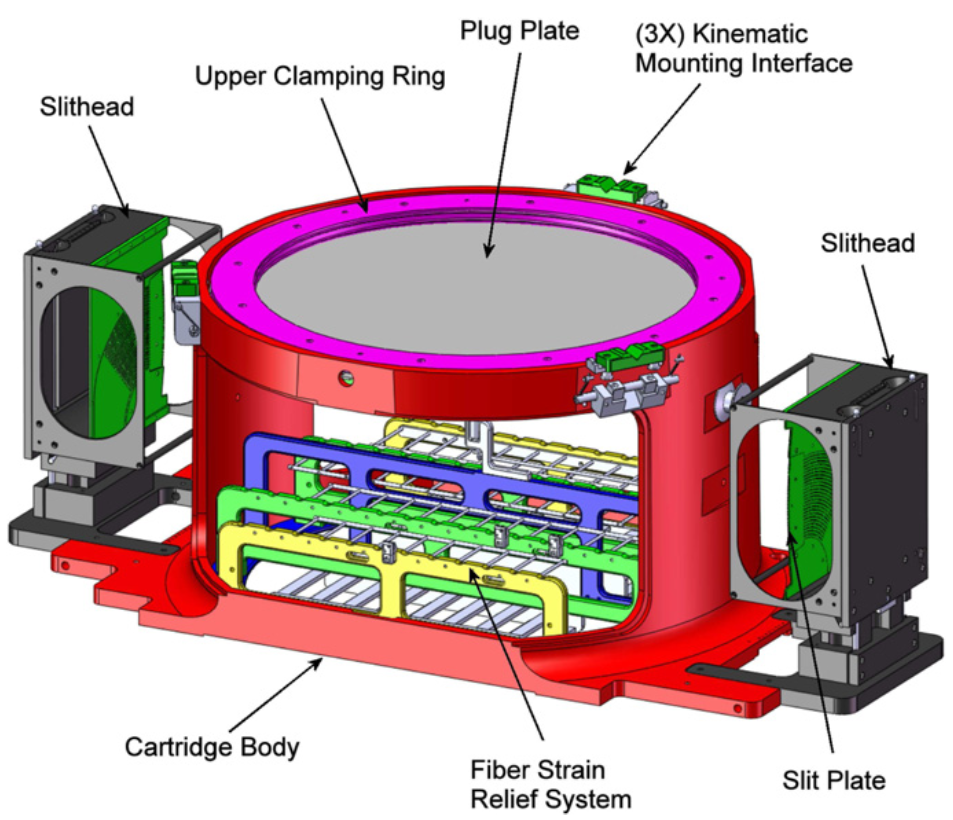
\includegraphics[width=0.7\textwidth]{fig/spectro/cartridge.png}
    \caption{Illustration of the SDSS cartridge holding the focal plane plate and the optical fibres. 
    Figure extracted from \cite{smeeMultiobjectFiberfedSpectrographs2013}. }
    \label{fig:cartridge}
\end{figure}
 
The light of the objects is transported by the optical fibres through the 
Sloan spectrographs, shown in Figure~\ref{fig:spectrograph}. 
There are two spectrographs attached at the focal plane
of the telescope. Each spectrograph receives the light from 500 fibres and passes 
it through a beam-splitter, dividing it into a red and blue channels. 
Each channel has is own grism that spreads the light over wavelength before
hitting the CCDs. The blue camera observes roughly from 3500 to 6000~\angstrom\ and the red
camera from 6000 to 10500~\angstrom. The resolution $R \equiv \lambda / \Delta \lambda$ 
increases with wavelength from 1500 to 2000 on the blue camera and from 2000 to 2500 
on the red camera. 

\begin{figure}
    \centering 
    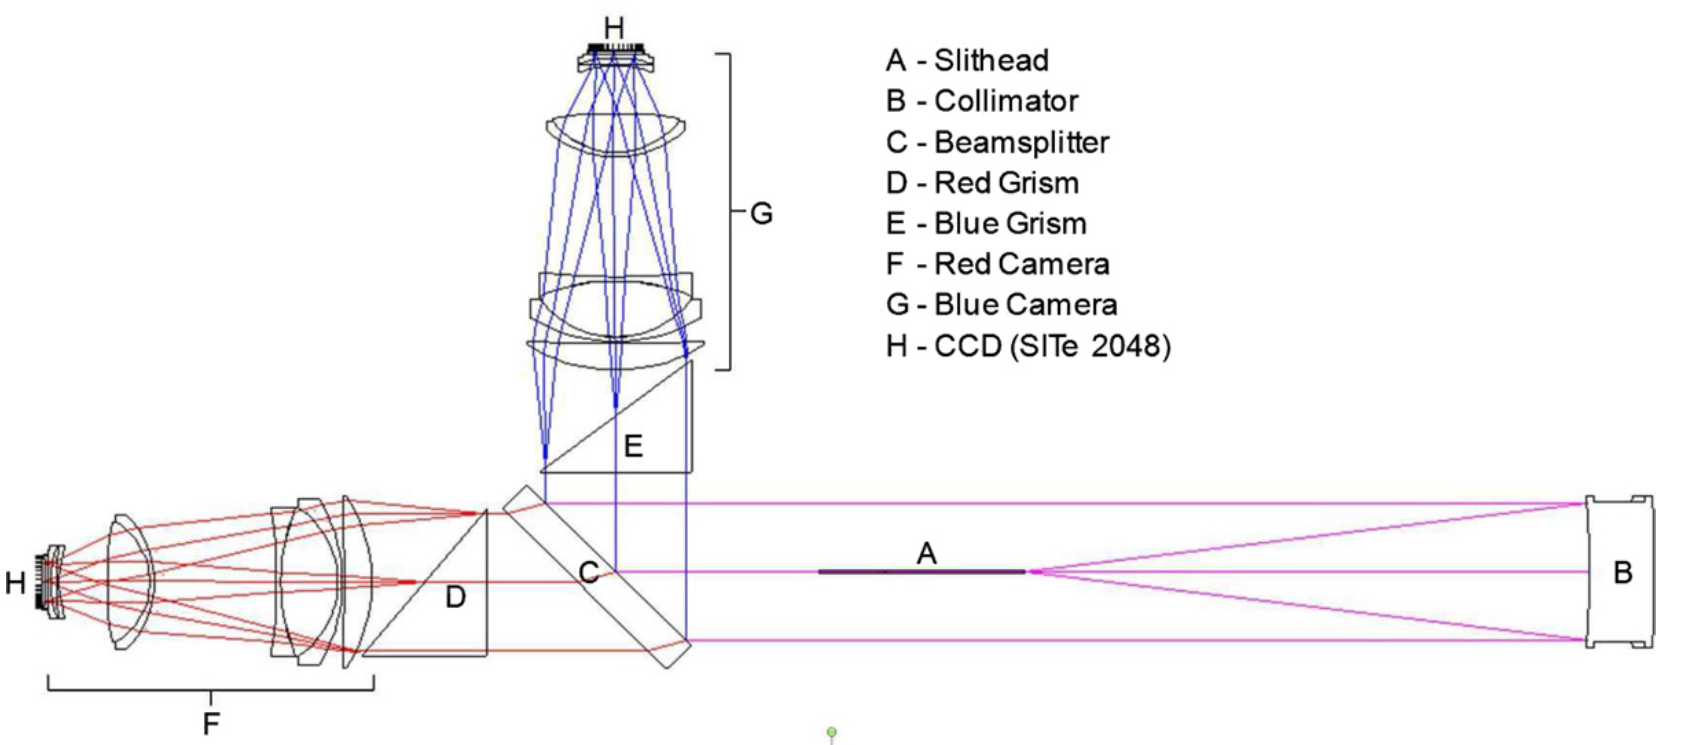
\includegraphics[width=\textwidth]{fig/spectro/spectrograph.png}
    \caption{Illustration of one SDSS spectrograph. 
    Light propagates from the slithead (also shown in Figure~\ref{fig:cartridge})
    towards the blue and red cameras. 
    Figure extracted from \cite{smeeMultiobjectFiberfedSpectrographs2013}. }
    \label{fig:spectrograph}
\end{figure}
 

In addition to the science exposures (observing galaxies), a small set
of calibration exposures is also taken, typically at the beginning and at the end 
of the observing run. Flat exposures are taken with lamps that emit over all 
wavelengths. The light is passed through the spectrographs, so we refer to these
as fibre-flats, as opposed to the exposures taken without the spectrographs, named 
super-flats. With another type of lamp, which emit narrow lines at some specific 
wavelengths, arc exposures are obtained, that are used to derive the relation between 
wavelength and CCD pixel location.

\section{From electrons to spectra}
\label{spectro:pipeline2d}

This section describes the data reduction pipeline of 
spectroscopic observations by the SDSS telescope, for which 
I contributed as the eBOSS Lead Data Scientist. 
This automated pipeline transforms the counts stored in CCDs into 
calibrated spectra, for which redshifts are estimated. 
Figure~\ref{fig:pipeline} displays a flowchart of the process. 
The software, named \texttt{idlspec2d}, was written in Interactive Data Language (IDL)
and can be found online\footnote{\url{https://svn.sdss.org/public/repo/eboss/idlspec2d/tags/v5_13_0/}}.
The latest version used in Data Release 16 
of eBOSS data is \texttt{v5\_13\_0} (\cite{ahumada16thDataRelease2020}).


\begin{figure}
    \centering 
    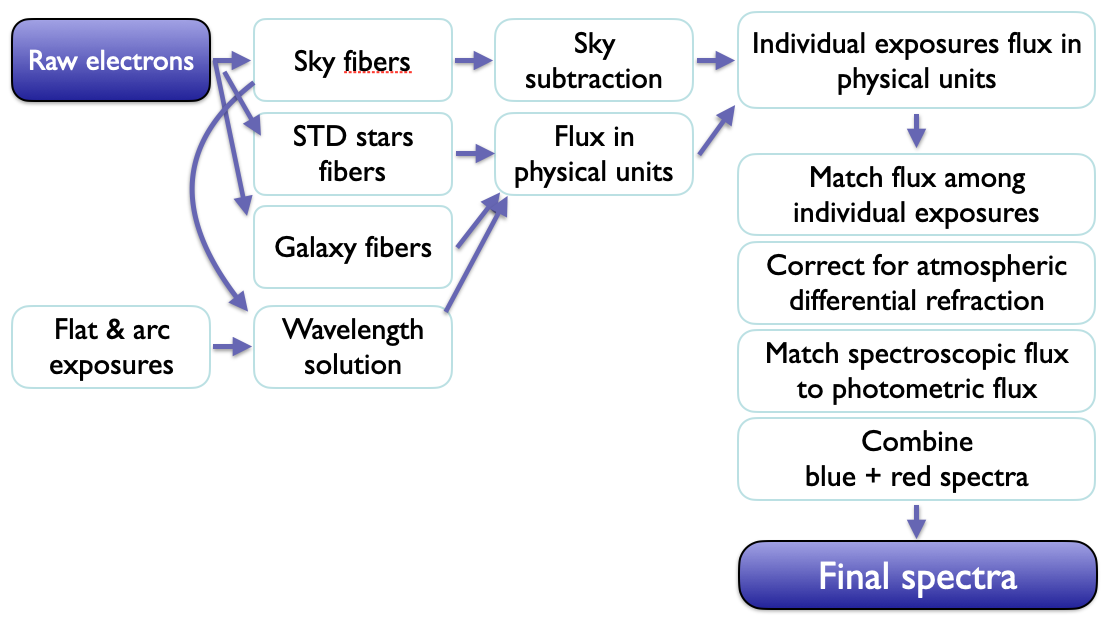
\includegraphics[width=\textwidth]{fig/spectro/pipeline_flowchart.png}
    \caption{Flowchart summarising the several steps of the automated data reduction pipeline from SDSS spectroscopic data.}
    \label{fig:pipeline}
\end{figure}
 

The dispersed light of each object falls onto CCD detectors containing 
2048x2048 square 24$\mu$m pixels. 
There are 500 traces per CCD, except when fibres are broken or unplugged by accident. 
The traces of each spectra are parallel and slightly curved towards the edges. 
They are separated by about 7 pixels. 

The first step of the data reduction is to remove bias and dark, mask 
cosmic rays and other known bad pixels, 
convert counts into electrons using estimated gain values, 
and correct for the super-flat image (flat taken without the spectrograph). 

The next step is to extract the total number of counts per wavelength and per object.
One of the axis of the CCD is aligned with the wavelengths, but we do not know the
wavelength solution at this point. The other axis is aligned with fibre number. 
The extraction of the fluxes is performed by bundles of 20 fibres. A set of 20 Gaussian
profiles plus a third order polynomial term are fit simultaneously over the counts. 
From the best-fit parameters of the Gaussian, one can compute the total flux at each 
wavelength for each object. This fit is performed regardless of whether the fibres contain 
flux from sky, stars or galaxies. 
The extraction step is performed similarly to science, flat and arc exposures. 


One important aspect of extraction is: what do we use as weights in the fit?
For SDSS-II and III, the extraction used the total estimated variance of each pixel,
assumed to be Poisson with mean equal to the number of observed hits in the pixel. 
However, in SDSS-IV eBOSS we pushed the limits of the instrument by observing fainter
objects. In this regime, we started to observe biases due to this weighting scheme in 
the extraction. The ideal extraction would use the true variance 
(\cite{horneOptimalExtractionAlgorithm1986}), not the estimated
one, as a weight. Using the estimated one yields a bias in the final fluxes. 
We modified the extraction algorithm such that it would use a flux-independent weight 
for the fit, yielding unbiased fluxes. Consequently, this extraction is less 
optimal, yielding slightly larger flux uncertainties. Biased fluxes affected 
particularly the analysis of \lya forests, as described in chapter~\ref{chap:forests}
or in the appendix of \cite{bautistaMeasurementBaryonAcoustic2017}.

The fibre-flat images are used to calculate the traces positions and widths 
(more precisely than in science images) 
and to correct for throughput variations across fibres. 
The arc images are used to calculate the wavelength solution and 
the dispersion in the wavelength direction based on the line widths. 
Sky lines in science exposures are eventually used to do small adjustments 
to the arc-image solution. 

The flux in the sky fibres are used to fit a sky model in units of counts.
A polynomial dependency over fibre index is used to account to variations 
over the focal plane. This sky model is then subtracted from all science 
spectra, including the sky spectra themselves and calibration stars. 
The sky-subtracted sky fibres are a good metric to evaluate the quality of 
sky subtraction algorithm. 

The next step of the reduction is the \emph{flux calibration}, 
which converts the observed counts into flux in physical units. 
The spectra of standard stars are the main ingredient of the flux calibration. 
The stars chosen for calibration are of type F, with small variations in 
temperature and metallicity. Physical models of their spectral emission 
including absorption features can be obtained via complex stellar synthesis calculations. 
The goal is to fit absorption lines to the data 
in order to determine the exact model for each observed star. 
We start by isolating the absorption lines in the observed spectrum 
(in units of counts) by fitting a smooth function over its shape, 
then dividing the whole spectrum by this model. 
This residual spectrum has only absorption features in an dimensionless scale.
The same is done for the physical stellar models. We fit these absorption features 
to all models to find the best star model for a given spectra.
Once the best-fit parameters of the star are found, 
a calibration vector is constructed by simply taking the ratio of 
the observed counts to the full model including its smooth component. 
A set of ten stars are fit independently and a single calibration 
vector is obtained from them. This final calibration vector is then 
applied to all other galaxy spectra in order to convert their number counts into
flux in physical units. During the last years of eBOSS, I updated 
the set of physical stellar models from the Kurucz catalogue to those used 
in DESI (\cite{allendeprietoCollectionModelStellar2018}) 
which have a larger diversity in stellar 
parameters and more precise absorption features. This update contributed
to a significant reduction of flux calibration residuals 
computed using stacks of spectral regions of quasars without emission 
or absorption lines. Figure~\ref{fig:flux_calibration_residuals} shows this 
improvement. 

\begin{figure}
    \centering
    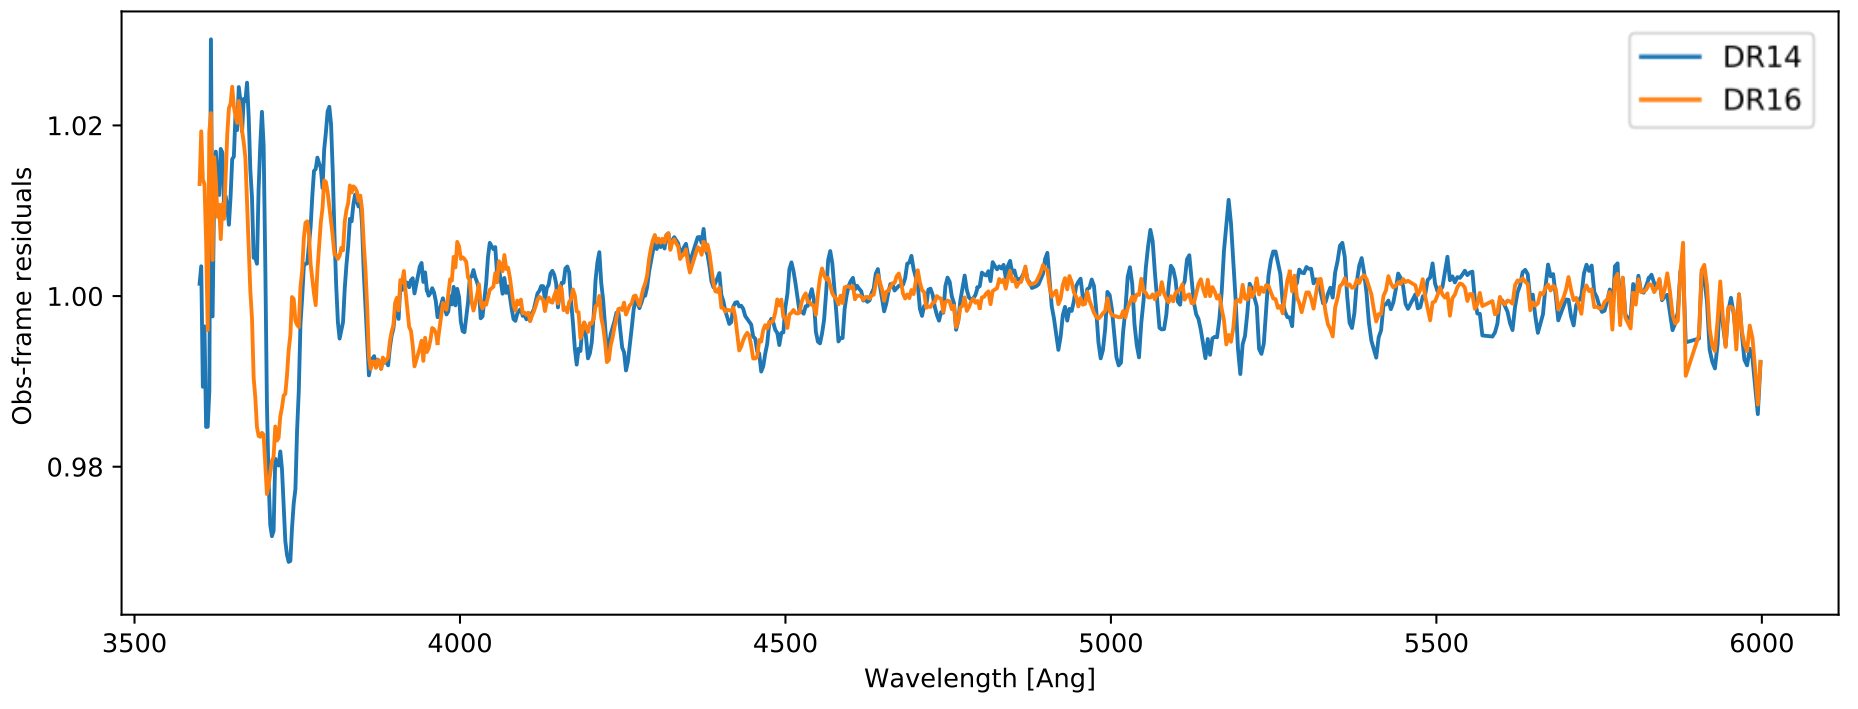
\includegraphics[width=\textwidth]{fig/spectro/picca_calibration_residuals_DR14_DR16_civ.png}
    \caption{Flux calibration residuals computed using an observer-frame stack of 
    quasar spectral regions without emission or absorption lines. 
    Two versions of the automated pipeline are displayed. The DR16 includes an 
    update of the stellar models used to fit spectra of standard stars. 
    We see a significant improvement in these residuals with this change. }
    \label{fig:flux_calibration_residuals}
\end{figure}

Once individual science exposures are converted into physical flux units, 
we proceed to the co-addition of these exposures into a single set of spectra. 
For a given object, a B-spline is fitted over all observed spectra, 
using a new wavelength grid with constant steps in $\log_{10} \lambda$ of $10^{-4}$. 
The best-fit spline is the final co-added spectrum for this object. 
The co-addition is made independently for each object. 
At this stage, we also combine spectra from blue and red cameras into 
one single spectrum covering the full wavelength range of 3500 to 10500 $\AA$. 
The last step of this process is the calculation of potential broadband 
distortions in flux caused by atmospheric differential refraction (ADR). 
Using information from the plate design, the position of the fibres in 
the plate and the actual observations (airmass, hour-angle), one can 
compute a correction vector that is also applied to all spectra. 

During the whole reduction, pixels or whole fibres can be masked due to any issues, 
or when the robustness of flux calculations is compromised. 
Each pixel has a flux and an uncertainty estimates. The latter is expressed 
as an inverse variance, which can be used directly as a weight in analyses.



\section{From spectra to redshifts}
\label{spectro:pipeline1d}

The next and last step of the automated data reduction pipeline is the 
spectral classification and redshift measurement. 
A set of physical templates of stars, galaxies and quasars is fit to 
each spectrum by a simple $\chi^2$ minimization. For each template, 
we scan over several values of redshifts to obtain the minimum $\chi^2$. 
The redshift ranges probed depend on the type of template: 
stellar templates are allowed to vary around $z =0$, 
galaxy templates are fitted over $0 < z < 2$ and quasar ones over $0 < z < 7$. 
The five best pairs of template and redshift producing the smallest $\chi^2$ values are stored. 
Redshift uncertainties are estimated using the $\chi^2$ profiles around the minima.
If the difference between the first and second best-fit $\chi^2$ values
is smaller than a certain threshold (corresponding to roughly 
5$\sigma$ for one parameter), a warning flag is set, meaning 
that the classification is not to be trusted. 
Figure~\ref{fig:spec1d} illustrates an example of $\chi^2$ profile versus redshift,
with the potential first and second best-fit redshifts and their uncertainty estimation. 

\begin{figure}
    \centering
    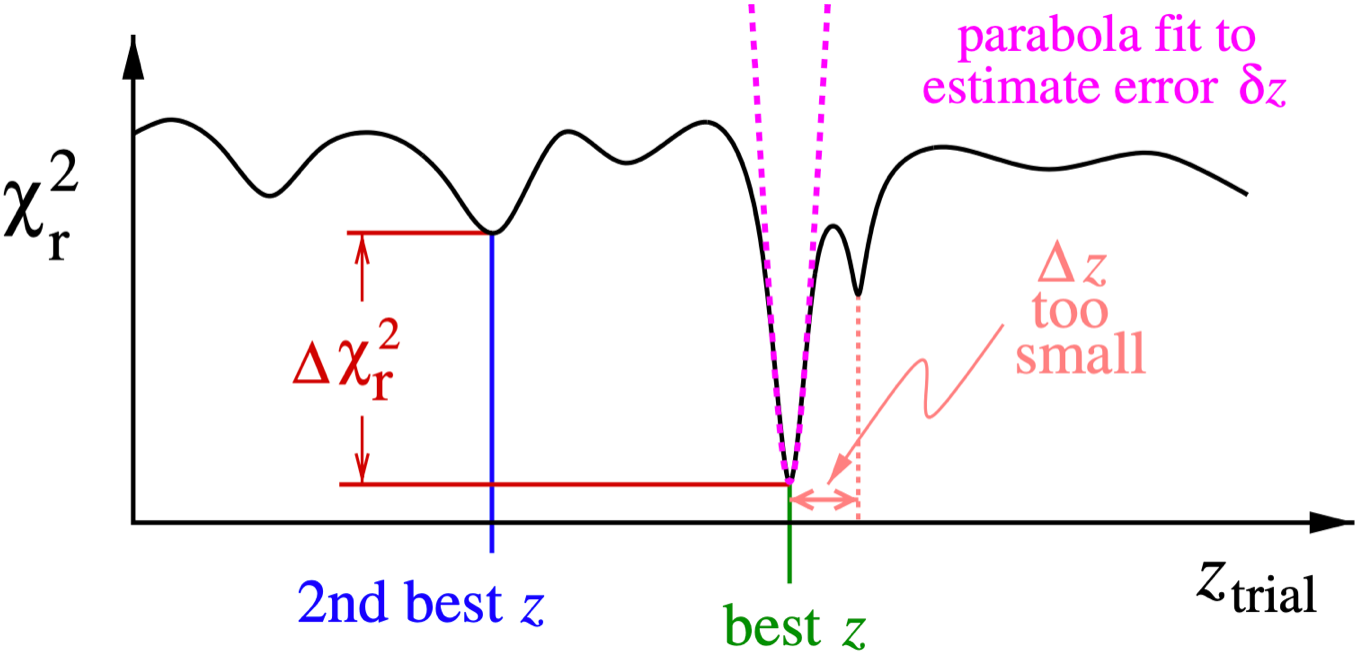
\includegraphics[width=0.7\textwidth]{fig/spectro/spec1d_chi2.png}
    \caption{Illustration of a $\chi^2$ profile for a spectral template versus redshift. 
    The best redshift is defined by the location of the global minimum (green). 
    Other minima separated by less than 1000~\kms are not considered to be separate (pink). 
    A parabolic fit to the global minimum (magenta) is used to determine redshift uncertainty. 
    The second-best redshift fit is determined by the location of the second-lowest well-separated minimum (blue). 
    The difference $\Delta \chi^2$ (red) between best and second-best fits is used 
    to quantify the confidence in the measurement.
    Figure extracted from \cite{boltonSpectralClassificationRedshift2012a}. }
    \label{fig:flux_calibration_residuals}
\end{figure}

A program of visual inspection of reduced spectra is carried out following the first observations 
of a new survey. 
Visual inspection is a important step in order to verify 
the quality of the data reduction, the automated classification and the redshift measurement. 
A truth table containing the visually confirmed redshifts and classifications
for thousands of spectra is one of the results of the visual inspection. 
This truth table is used to compute the actual density of tracers that are 
obtained for a given target selection, as a function of redshift. 
Spectral features caused by problems in the reduction were then reported to the
pipeline team. 

During the first months of eBOSS, I coordinated a program of 
visual inspection where about 15 members analysed about a thousand spectra each
(with some overlap for cross-checking). This provided a truth table
for the Luminous Red Galaxies from eBOSS. Similar programs were carried out
for the eBOSS Emission Line Galaxies and quasars. The inspections of eBOSS quasars
continued throughout the whole program, where a small fraction of
the spectra without confident automated classifications were inspected.
In DESI, a larger visual inspection program was put in place for the same goals.

This concludes the description of a spectroscopic survey: 
a machine converting photons to redshifts useful for cosmology.  

	\chapter{ The high-redshift Universe and its forests }
	\label{chap:forests}
	\chaptertoc{}

The high-redshift Universe ($2<z<4$) could be explored, until now, thanks
to the Lyman-$\alpha$ forests. 

\section{Forests as a tracer of neutral hydrogen}

\section{Statistics of the absorption}

\section{Baryon acoustic oscillations in the forests}

\section{Weak-lensing of forests}

\section{Impact of redshift errors}




	\chapter{ The mid-redshift Universe and its galaxies }
	\label{chap:galaxies}
	\chaptertoc{}

\vspace{1em}

At redshifts between 0 and 2, galaxies can be used as tracers of
the matter distribution. With the statistics of the galaxy distribution 
we can measure characteristic scale of the baryon acoustic oscillations (BAO), 
as well as extract information about the growth-rate of structures from 
the anisotropies caused by redshift-space distortions (RSD). 
As presented in Chapter~\ref{chap:intro}, BAO and RSD are powerful 
probes of dark-energy and theories of gravity. 

In this Chapter, I overview my contributions for the study of dark-energy 
with galaxy clustering. Section~\ref{galaxies:catalogue} describes how to 
create a galaxy clustering catalogue from the spectroscopic observations, 
including and correcting for most observational systematic effects.
In section~\ref{galaxies:bao} I present the BAO measurements I performed 
with the SDSS sample of luminous red galaxies, while section~\ref{galaxies:rsd}
focus on the RSD constraints. Section~\ref{galaxies:joint} 
overviews recent work carried out by my PhD students Tyann Dumerchat 
and Vincenzo Aronica on the joint analysis of galaxy clustering in 
Fourier and configuration space. 

The work described in this chapter is published in the following 
articles: 
\cite{bautistaSDSSIVExtendedBaryon2018, 
bautistaCompletedSDSSIVExtended2020,
gil-marinCompletedSDSSIVExtended2020,
rossCompletedSDSSIVExtended2020,
zhaoCompletedSDSSIVExtended2021,
%dumerchatJoint2022
}. 

\section{From redshifts to clustering catalogues}
\label{galaxies:catalogue}

An essential step in the cosmological analysis of galaxy survey data is 
to convert convert a list of galaxy redshifts (see Chapter~\ref{chap:spectro}) 
into a catalogue from which we can define overdensities 
$\delta_n(\vec{x}) = n(\vec{x})/\bar{n} - 1$, where $n(\vec{x})$ is the 
number density 
of galaxies in a volume element located at position $\vec{x}$. 
The quantity $\bar{n}$ is the average galaxy number density over the probed 
\emph{volume}. Therefore, it is important to 1) define precisely what is the 
volume observed, or in jargon terms, the survey window function; and 
2) to make sure that the number density of galaxies is tracing the actual 
cosmological fluctuations and not any spurious contamination. 

The simplest form of survey window function would be some function of position $\vec{x}$ 
that is 1 if the volume was ``observed'' and 0 else. 
One way to define this function is using a Poisson random sampling 
of the volume with points, with some arbitrary higher number density than the 
galaxy average number density (typically between 20 or 50 times higher). 
The list of points is referred to as the \emph{random} catalogue. 
In practice, the random catalogue is more complicated and accounts for 
observational completeness and systematic effects, as described below. 

In SDSS analyses, the random catalogue is a combination of an angular footprint 
and a radial distribution, both trying to matching the galaxy sample as better as possible. 

I describe now the procedure to define the angular footprint. 
The starting footprint is the same where the target selection 
(section~\ref{spectro:target})
was previously defined. 
Figure~\ref{fig:eboss_footprint} displays the eBOSS footprint for the three tracers 
(LRGs, ELGs and QSOs) compared to the BOSS footprint and the stellar density map from Gaia. 
Regions with bad photometric or around 
bright stars are masked out by removing randoms belonging to these regions
(or assigning them a null weight). 
After tiling, fibre assignement and spectroscopic observations, the footprint 
can be divided into an unique set of sectors. Each sector corresponds to regions
observed by one or more plates. The \emph{fibre completeness} of each sector is 
defined as the ratio between the number of spectroscopically observed targets and 
the number of available targets in the sector. Random points are sub-sampled or de-weighted 
following the fibre completeness to account for it. 

\begin{figure}
    \centering 
    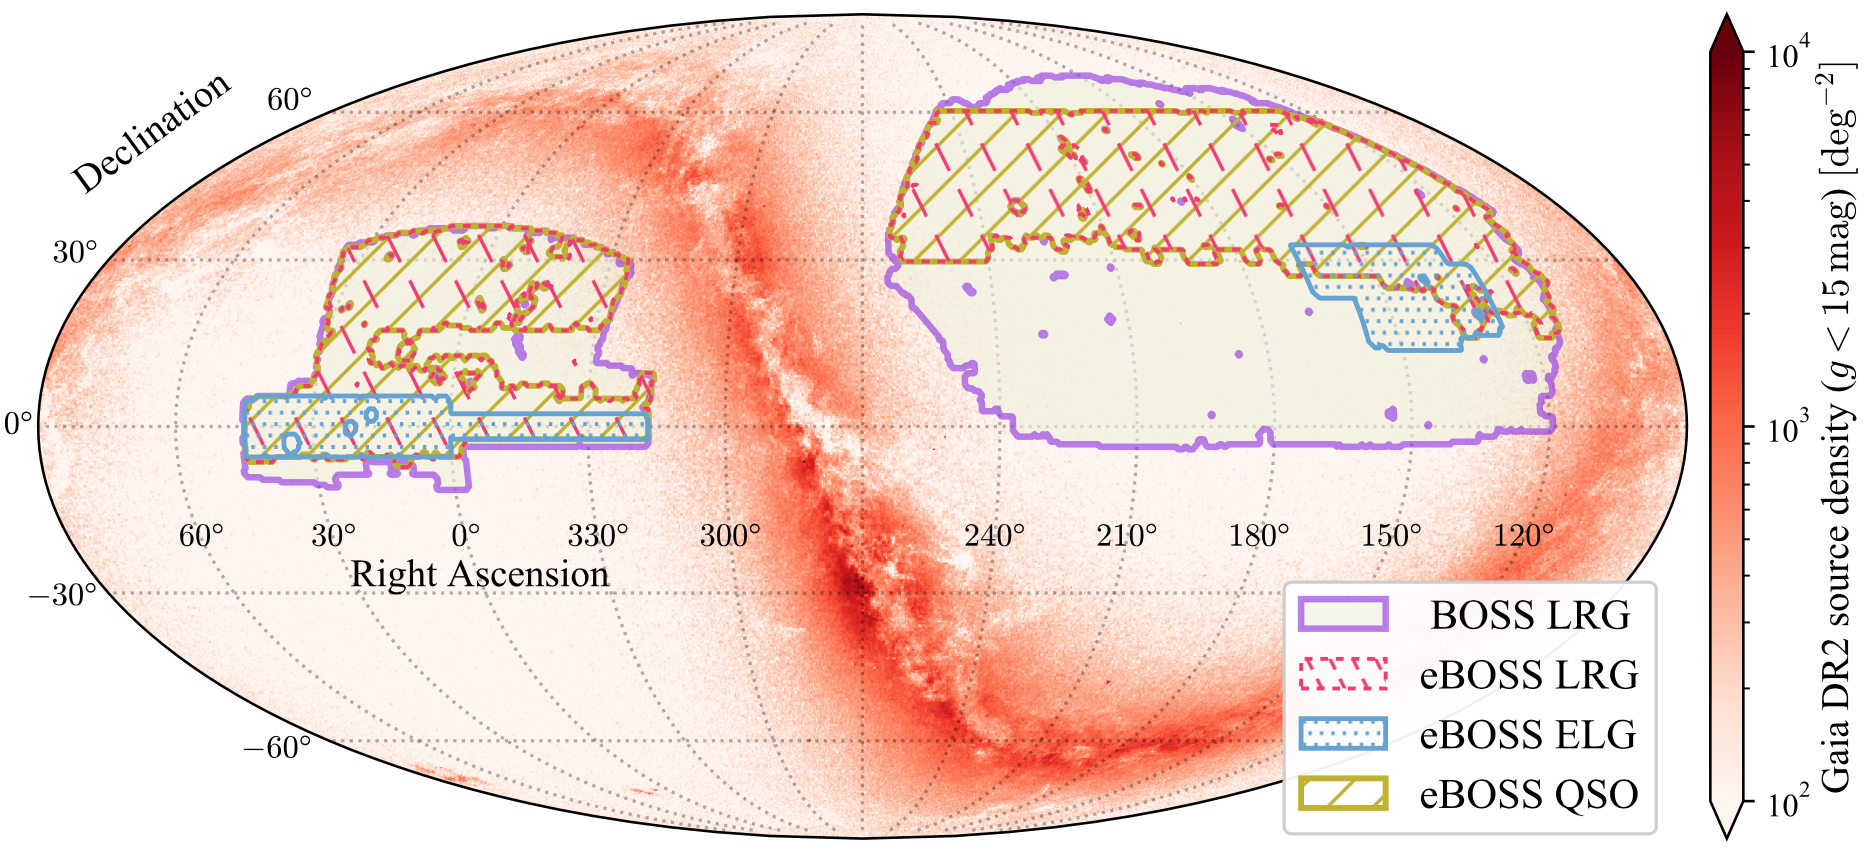
\includegraphics[width=0.9\textwidth]{fig/galaxies/eboss_footprint.png}
    \caption{ The DR16 footprint for each eBOSS tracer: Luminous Red Galaxies (LRG), 
    Emission Line Galaxies (ELG) and quasars (QSO). The BOSS DR12 LRGs area is also shown, 
    as well as the density map of Gaia DR2 sources with $g < 15$ mag.
    Figure extracted from \cite{zhaoCompletedSDSSIVExtended2021}.} 
    \label{fig:eboss_footprint}
\end{figure}

Some targets cannot be observed due to 
its proximity to another observed target and the finite size of fibres, corresponding 
to 62 arcseconds in the sky. We refer to these events as \emph{fibre collisions}. 
Collisions might happen not only to pairs of galaxies, but to any group of targets with 
linking lengths smaller than 62 arcsec. Depending on the number of plates observing 
a giving sector, some collisions might be solved but the missing ones might 
impact the measured clustering on small scales if not corrected. 
While there are several methods to solve collisions 
(\cite{guoNewMethodCorrect2012, bianchiUnbiasedClusteringEstimation2017}),
we used the simplest up-weighting technique, where the nearest observed galaxy 
is up-weighted by the number of non-observed targets within the collision group. 
This assumes that non-observed targets are also galaxies of the same target type and 
that they are physically close (angularly and radially) to the observed ones.
On scales above a few \hmpc, this simple correction is a good approximation. 

Two additional sets of weights are defined to correct for spurious density 
fluctuations which contaminate the cosmological fluctuations. 
These weights are applied to the galaxies themselves. 

The first set of weights corrects for angular fluctuations caused 
by correlations between galaxy number density and photometry-related quantities,
such as Galactic extinction, stellar density, imaging depth or sky flux.
They are commonly referred to as \emph{photometric weights}. 
Figure~\ref{fig:photo_systematics_lrg} displays these correlations 
for the LRG sample both before and after corrections. 
For the analysis of eBOSS DR16 LRGs, I have 
implemented\footnote{\url{https://github.com/julianbautista/eboss_clustering/blob/master/python/systematic_fitter.py}} 
a multi-dimension 
linear regression that assumes these correlations are linear and 
accounts for the fact that some photometric quantities are correlated between themselves 
(e.g., stellar density and Galactic extinction).
This multi-linear method is based on work described in \cite{prakashSDSSIVExtendedBaryon2016}.
Of course, more advanced methods have been developed since then, based on 
machine learning algorithms 
(\cite{rezaieImprovingGalaxyClustering2020, chaussidonAngularClusteringProperties2021}).
It is important to evaluate the performance of these algorithms with mock catalogues
where we add artificial contamination 
and quantify how well we recover the initial raw power spectrum after correcting for them. 
There is a risk of overfitting and removing some large-scale cosmological modes which 
can be harmful for clustering analysis, particularly those aiming at measuring 
primordial non-Gaussianity 
(\cite{rezaiePrimordialNonGaussianityCompleted2021, muellerClusteringGalaxiesCompleted2021}).

\begin{figure}
    \centering 
    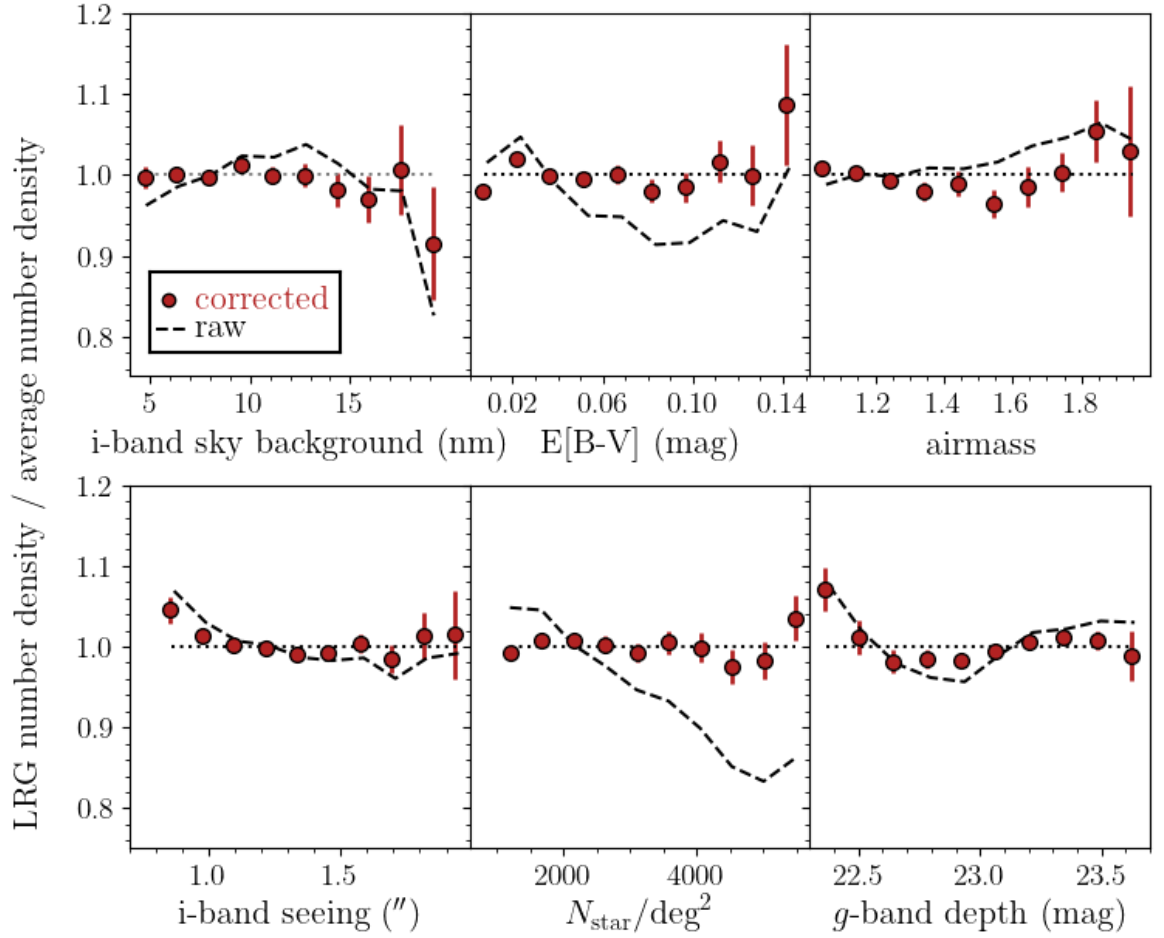
\includegraphics[width=0.7\textwidth]{fig/galaxies/photometric_weights_lrg.png}
    \caption{ Fluctuations in the angular LRG density as a function of 
    various imaging properties and Galactic foregrounds. 
    The dashed curves show these fluctuations before any correction 
    while red points show the result of applying a linear correction for 
    stellar density and Galactic extinction. 
    Figure extracted from \cite{rossCompletedSDSSIVExtended2020}.} 
    \label{fig:photo_systematics_lrg}
\end{figure}

A second set of weights corrects for the fact for the so-called \emph{redshift failures}, 
i.e., the fact that some spectra with low signal-to-noise ratio (S/N)
do not yield a statistically significant redshift measurement. 
If they were randomly distributed across the sky, failures would not be an issue for 
clustering. However, given the instrument configuration and throughput, these failures 
imprint a pattern in the sky which contaminates clustering. 
In the left panel of Figure~\ref{fig:eboss_zfailures} we see the average failure rate 
of eBOSS LRGs as a function of position in the focal plane. The reason for this pattern
is that the fibres at the side edges of the focal plane transport light to the edges 
of the camera CCDs and therefore have a lower-than-average throughput, or lower signal-to-noise
ratio. 
The right panel of Figure~\ref{fig:eboss_zfailures} shows the 
dependency of the average redshift failure rate as a function of the signal-to-noise
ratio of the observation\footnote{The signal-to-noise ratio of an observation is 
a function of the signal-to-noise ratio of all observed spectra and their magnitudes.}, 
which is the actual underlying reason for the failure rates. 
When modelling these dependencies of failure rates with S/N (or fibre number or focal plane
position), one can correct these spurious fluctuations by assigning a weight 
inversely proportional to the modelled rate. 
These are the so called \emph{redshift-failure weights} and are assigned to the 
galaxies with confident redshift measurements, to compensate for the eventual 
non-confident ones at the same location in the focal plane. 

\begin{figure}
    \centering 
    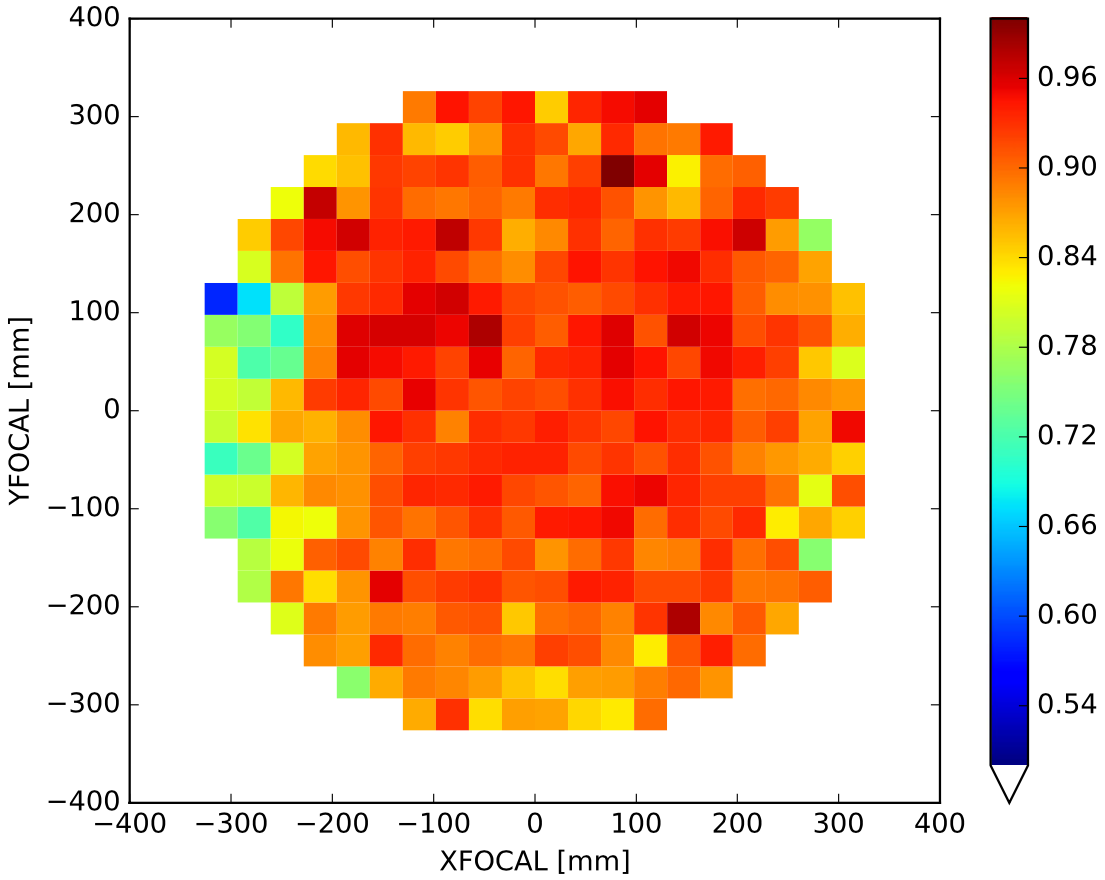
\includegraphics[width=0.49\textwidth]{fig/galaxies/eboss_z_failures_focalplane.png}
    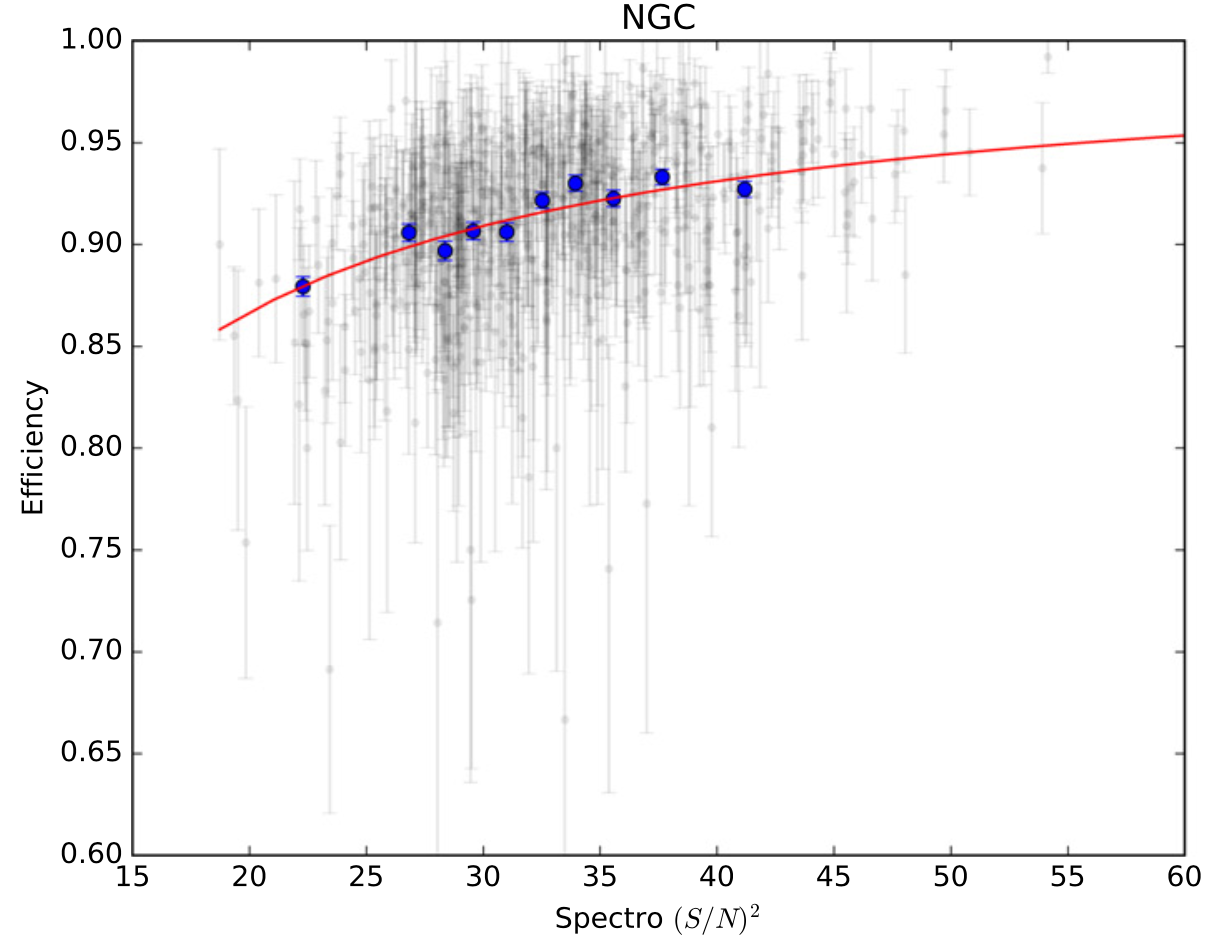
\includegraphics[width=0.49\textwidth]{fig/galaxies/eboss_z_failures_sn.png}
    \caption{ 
        Average redshift efficiency as a function of physical position of the optical 
        fiber in the focal plane (left panel) and as a function of the observation
        signal-to-noise squared (right panel).  
        The left panel shows how redshift-failures imprint a pattern on the sky 
        and therfore must be corrected. The right panel shows the underlying reason 
        for the failures. The model (red line) is used to compute correction weights.
    Figures extracted from \cite{bautistaSDSSIVExtendedBaryon2018}.} 
    \label{fig:eboss_zfailures}
\end{figure}

Once all galaxies have their correction weights (fibre collision, photometric and 
redshift-failure) and the randoms are corrected by fibre completeness, 
the radial selection function. The idea is to assign redshifts to randoms 
such that they follow the same redshift distribution as the galaxies. 
The redshift distribution is often quantified by the comoving galaxy (weighted)
number density $\bar{n}(z)$. 
Figure~\ref{fig:eboss_z_distrib} shows the comoving density of eBOSS tracers 
as a function of redshift. 
For randoms to match this distribution, we randomly assign the actual galaxy 
redshifts to each random, with repetition. Another possibility is to 
fit some smooth function over the observed $\bar{n}(z)$ and draw random redshifts
from the resulting model. In any case, these methods will introduce the so called 
\emph{radial integral constraint}, i.e., the fact that the observed $\bar{n}(z)$ is 
not the true ensemble averaged function of the Universe, it is just one 
volume-limited realisation of it. The impact on clustering of the radial integral 
constraint is inversely proportional to the area of the footprint
(\cite{demattiaIntegralConstraintsSpectroscopic2019}) and it is significant 
for surveys such as the eBOSS ELG (see Figure~\ref{fig:eboss_footprint} and 
\cite{tamoneCompletedSDSSIVExtended2020, demattiaCompletedSDSSIVExtended2021}). 


\begin{figure}
    \centering 
    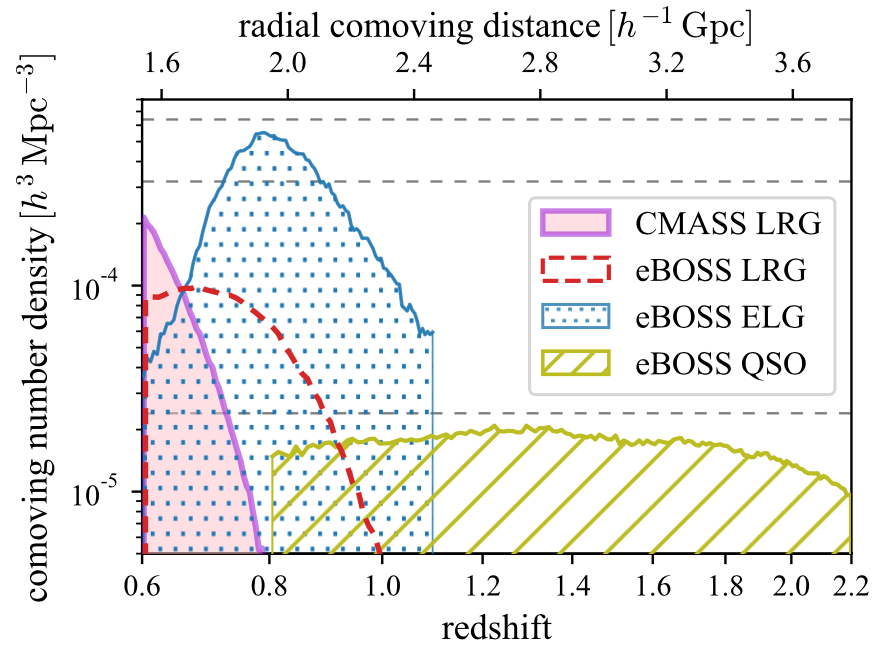
\includegraphics[width=0.6\textwidth]{fig/galaxies/eboss_z_distribution.png}
    \caption{ The weighted comoving number densities $\bar{n}(z)$ of eBOSS DR16 tracers
    and BOSS DR12 CMASS LRGs, with all the photometric and spectroscopic
    systematic weights included. 
    The comoving distances and volumes are computed assuming a flat-$\Lambda$CDM 
    cosmology with $\Omega_m = 0.31$. 
    %The three horizontal dashed lines show the number densities of the cubic LRG, ELG, and QSO    
    %EZmockcatalogues,i.e. $3.2 \times 10^{-4}$, $6.4 \times 10^{-4}$, and $2.4 \times 10^{-5} h^3 \text{Mpc}^{-3}$, respectively.
    Figure extracted from \cite{zhaoCompletedSDSSIVExtended2021}.} 
    \label{fig:eboss_z_distrib}
\end{figure}

The final step of the catalogue consists in adding an additional set of weights 
to galaxies that optimise the signal-to-noise ratio of clustering measurements 
when the redshift distribution is not uniform. These weights were first introduced 
by \cite{feldmanPowerSpectrumAnalysisThreedimensional1994} and have been applied 
to all clustering analysis ever since. They are commonly referred to as 
\emph{FKP weights} and can be written for a galaxy $i$ as
\begin{equation}
    w_\text{i, FKP} = \frac{1}{1 + \bar{n}(z_i)P_0}
\end{equation}
where $P_0$ is a rough value of the power spectrum of the tracers at some 
particular scale of choice, usually BAO scales for large-scale clustering measurements.
For eBOSS analyses, we chose a scale of $k \sim 0.1 h\, \text{Mpc}^{-1}$ for which 
$P_0 = 10000 h^{-3}\text{Mpc}^{3}$ for LRGs, 
$P_0 = 4000 h^{-3}\text{Mpc}^{3}$ for ELGs and 
$P_0 = 6000 h^{-3} \text{Mpc}^{3}$ for QSOs. 

As summary, the random catalogue describes the angular and radial selection functions
of the galaxy survey. 
Each random has a weight $w_r = w_\text{comp} w_\text{FKP}$, where $w_\text{comp}$ accounts
the spectroscopic completeness of targets and $w_\text{FKP}$ are optimal weights for clustering. 
Each galaxy has a weight given by $w_g = w_\text{col} w_\text{photo} w_\text{fail} w_\text{FKP}$,
where $w_\text{col}$ accouns for fibre collisions, $w_\text{photo}$ corrects fluctuations caused 
by photometry and $w_\text{fail}$ corrects redshift failures. 
These weights are used computing correlation functions or power spectra (see~\ref{galaxies:clustering}).

\section{Reconstruction of linear density field} 
\label{galaxies:reconstruction}

Bulk motions of galaxies on scales of tens of Mpc impact their two-point statistics, 
acting as a smoothing of the clustering (\cite{eisensteinRobustnessAcousticScale2007}).  
These motions smooth/broaden the BAO peak, reducing the precision on our measurement of its position. 
In the past decades, several methods have been proposed to reconstruct
the linear density field and remove these bulk motions from a galaxy survey,
therefore sharpening the BAO peak.
These methods are referred to as \emph{reconstruction} methods. 
Reconstruction is now an essential part of standard BAO measurements from galaxy surveys,
since they improve significantly their precision. 

The simplest form of reconstruction is based on a theoretical relationship between 
the galaxy density field on large scales (our observable) and the displacement field connecting 
the observed field (Eulerian frame) to its past version (Lagrangian frame). 
Lagrangian perturbation theory (LPT) can predict these displacements 
(see \cite{bernardeauLargeScaleStructureUniverse2002} for a review). 
To first order, the relation between displacements and density is linear 
(\cite{zeldovichGravitationalInstabilityApproximate1970}) and works quite well in 
recovering the linear BAO peak 
(\cite{nusserTracingLargeScaleFluctuations1992, eisensteinImprovingCosmologicalDistance2007}).
The first order LPT reconstruction is often called \emph{Zeldovich reconstruction}. 
Extending to second order LPT does not improve BAO reconstruction significantly 
(\cite{seoHighprecisionPredictionsAcoustic2010}) but it helps on recovering the 
velocity field (\cite{kitauraEstimatingCosmicVelocity2012}).
Zeldovich reconstruction has been used in all BAO measurements from SDSS (BOSS and eBOSS).
I implemented a python version\footnote{\url{https://github.com/julianbautista/eboss_clustering/}} of 
the Zeldovich reconstruction that uses Fast Fourier Transforms while accounting for the 
large angle effects 
(\cite{burdenEfficientReconstructionLinear2014, burdenReconstructionFourierSpace2015}). 
Alternatively, displacements can be computed 
in configuration space using finite difference approximations (\cite{padmanabhanCentDistance352012})
though these are slower and less precise than iterative FFTs. 

Since we do not observe the actual density of matter, an assumed bias relation between galaxy number density 
and matter density has to be assumed in reconstruction. Usually we assume a linear bias relation, where the 
bias value is estimated from the clustering of the standard galaxy catalogue. This is a reasonable approximation 
since reconstruction uses fluctuations on scales larger than $\sim 15$\hmpc. 
If one wants to remove redshifts-space distortions, one has to assume a value for the growth-rate of structures $f$
(see section~\ref{intro:probes:rsd}) in order to convert displacements into velocities. 
Therefore, the clustering of reconstructed catalogues depend on the fiducial values of bias and $f$, 
but less on the distance-redshift relation (\cite{carterImpactFiducialCosmology2020}). 

There are other backward reconstruction techniques such as those based on the least action principle (LAP).
First proposed by \cite{peeblesTracingGalaxyOrbits1989}, it was extended to cosmological applications 
by \cite{nusserLeastActionPrinciple2000, sarpaBAOReconstructionSwift2019}. 
\cite{sarpaExtendedFastAction2021} applied it for the BAO measurement of the BOSS DR12 galaxy sample. 

Reconstruction is essential to improve the precision on BAO measurements. However, 
due to imperfections in recovering the true initial conditions, 
reconstruction has not yet been used in attempts to derive cosmological 
constraints from the full-shape of the reconstructed two-point statistics.
Therefore, analysis of redshift-space distortions are based on the non reconstructed 
clustering (see section~\ref{galaxies:rsd}).  

\section{Mock catalogues}
\label{galaxies:mocks}

An important limitation in cosmology is that we only have a single realisation of our Universe. 
Therefore simulations are an essential tool to overcome this limitation. 

We can recognise two types of simulations mainly used in cosmology. First, 
n-body simulations (eventually including gas) solve numerically for the formation of structures
and are computationally expensive. They focus on the fully non-linear aspects and require a 
higher resolution setting, preventing them to simulate very large volumes or producing numerous 
realisations. N-body simulations are still the baseline for tests of perturbation theory models. 
The second type of simulations are the so-called \emph{mock catalogues} or simply \emph{mocks}. 
They are lower resolution and do not fully describe the non-linear clustering but they are 
faster to produce both in large volumes and in large number of realisations.
Their are key for the understanding of biases in best-fitted quantities and on their uncertainties. 
Given the large number of realisations, mocks have been used to estimate covariance matrices of 
clustering. Also, mocks allow us to study statistically the impact of observational systematic effects on our 
measurements. The last cosmological measurements from galaxy surveys have all an associated set of 
n-body simulations and a set of mock catalogues. I will describe the example I was involved in, 
the case of \textsc{EZmocks} produced for the eBOSS DR16 clustering measurements. 

A set of 1000 \textsc{EZmock} realisations was used in eBOSS DR16 clustering measurements 
for LRGs, ELGs and QSOs. They are fully described in \cite{zhaoCompletedSDSSIVExtended2021}. 
These mocks employ an effective Zeldovich approximation to evolve 
the density field in longer time steps (\cite{chuangEZmocksExtendingZel2015}). 
By construction, these mocks match the large-scale clustering 
of the target data sample, both 2 and 3-point statistics. 
They have some extra free parameters to simulate a biased galaxy sample. 
The eBOSS \textsc{EZmocks} also include light-cone effects produced by interpolating boxes
at different redshifts. 

The last step in the production of \textsc{EZmocks} was the addition of systematic effects. 
I was responsible of implementing all known observational effects from the data. 
A simple script\footnote{\url{https://github.com/julianbautista/eboss_clustering/blob/master/bin/ezmocks_add_systematics.py}}
gathers the information from the real catalogues and simulates fibre collisions, spurious 
fluctuations caused by photometry and spectroscopy (redshift failures). 
These contaminated mocks are then corrected using the same algorithms as for the real data, 
as described in section~\ref{galaxies:catalogue}. The clustering before and after adding 
those effects is extensively compared to real data (\cite{zhaoCompletedSDSSIVExtended2021}) 
and the agreement is found to be excellent on the scales of interest for BAO and RSD measurements. 



\section{From catalogues to clustering estimates}
\label{galaxies:clustering}

Once the catalogue of galaxies and the associated random catalogue are ready, 
any statistical quantity can be computed, such as $n$-point statistics. 
As discussed in section~\ref{intro:lss}, these statistics can be computed 
in either configuration space or Fourier space. 
This section describes how to obtain 2-point function estimates, 
in both spaces, which are the statistics I worked with. 

\subsection{Correlation function}
\label{galaxies:clustering:correlation_function}

The estimate of the correlation function $\xi(\vec{r})$ is based on counting pairs of galaxies 
in bins of separation $\vec{r}$ and comparing it to same numbers obtained from the random catalogue. 
For the estimator we use, there is no need to calculate galaxy number densities $n(\vec{x})$  
or overdensities $\delta_n(\vec{x})$ in some mesh. To optimise the variance of the estimator 
while keeping it unbiased, \cite{landyBiasVarianceAngular1993} proposed to include the cross-pairs  
between galaxies and randoms in the estimator, yielding:
\begin{equation}
 \xi(\vec{r}_i) = \frac{DD(\vec{r}_i) - 2DR(\vec{r}_i)}{RR(\vec{r}_i)} + 1,
 \label{eq:landy-szalay}
\end{equation}
where $DD(\vec{r}_i)$ (or $RR(\vec{r}_i)$) are the normalised paircounts between galaxies (or randoms) 
at bin $i$ corresponding to separation $\vec{r}_i$, 
$DR(\vec{r}_i)$ is the normalised cross-paircounts between galaxies and randoms. 
The normalisation of the paircounts is given by the total number of unique pairs in the catalogue, 
i.e., $N(N-1)/2$ if the catalogue contains $N$ galaxies or $N_g N_r$ for the cross pairs. 
When using weights as described in section~\ref{galaxies:catalogue}, nothing changes except 
that each pair of galaxies (or randoms) are weighted as $w_{ij} = w_i w_j$, where $w_i, w_j$ are the 
weights of each element of the pair. 

More recently, new ways to account for fibre collisions 
or incompleteness have been proposed 
(\cite{bianchiUnbiasedClusteringEstimation2017, percivalUsingAngularPair2017}) where each pair 
of galaxies would have a weight $w_{ij} \neq w_i w_j$, i.e., not a product of individual weights. 
This makes the calculation slighly slower since these weights have to be defined for each pair. 
These new estimators were first used with the eBOSS tracers
(\cite{mohammadCompletedSDSSIVExtended2020}) and are currently being employed within DESI. 

The estimator in Eq.~\ref{eq:landy-szalay} changes slightly when dealing with catalogues 
resulting from reconstruction algorithms,
where both galaxies and randoms are shifted in order to reduce the impact of bulk motions 
(see section~\ref{galaxies:reconstruction}). 
The Landy-Szalay estimator is now written as  
\begin{equation}
    \xi^\text{recon}(\vec{r}_i) = \frac{DD(\vec{r}_i) - 2DS(\vec{r}_i) + SS(\vec{r}_i)}{RR(\vec{r}_i)},
    \label{eq:landy-szalay-recon}
\end{equation}
where $S$ represents the shifted random catalogue and the $R$ is the usual random catalogue as before. 
See \cite{padmanabhanReconstructingBaryonOscillations2009, padmanabhanCentDistance352012} 
for a detailed derivation of this estimator. 

Most analyses of the two-point correlation function do not use the full $\xi(\vec{r}_i)$,
where $\vec{r}_i$ are bins in 2D separations such as bins in $(\rpara, \rperp)$ or $(r, \mu_r)$.
Most analysis further compress the estimated correlation function into a new basis with fewer 
degrees of freedom. Some analyses uses the correlation function 
\emph{wedges} $\xi_{\mu_{r1}, \mu_{r}}(r)$, which are 
averages of $\xi$ over $\mu_{r1} < \mu < \mu_{r2}$, as already discussed in section~\ref{forests:bao:correlations}. 
Other analyses, such as the one described in this chapter, decompose $\xi$ into a basis of 
Legendre polynomials $L_\ell(\mu_r)$ such that $\xi(r, \mu_r) = \sum_\ell \xi_\ell(r) L_\ell(\mu_r)$, 
where $\xi_\ell(r)$ are the correlation function \emph{multipoles}. 
Usually two or three wedges or multipoles are considered when comparing to clustering models.  

One of the most recent codes to compute correlation function accounting for all 
features described above is 
\textsc{pycorr}\footnote{\url{https://github.com/cosmodesi/pycorr}} 
which is being currently developed for DESI.

\subsection{Power spectrum}
\label{galaxies:clustering:power_spectrum}

The power spectrum is the analogous of the correlation function in Fourier space. 
It requires a Fourier Transform of the galaxy overdensity field, which introduces 
some effects that have to be correctly taken into account when fitting for clustering models. 
The power spectrum estimation is based on work by 
\cite{feldmanPowerSpectrumAnalysisThreedimensional1994,
bianchiMeasuringLineofsightdependentFourierspace2015,
handOptimalFFTbasedAnisotropic2017} and it is shortly described here. 

The first step is to assign galaxies and randoms into a three-dimensional mesh, 
defining an ``overdensity'' function $F(\vec{x}_i)$ as 
\begin{equation}
    F(\vec{x}_i) = w_\text{FKP}(\vec{x}_i) \left[ n(\vec{x}_i) - \alpha n_\text{rand}(\vec{x}_i) \right],
    \label{eq:overdensity_fourier}
\end{equation}
where $w(\vec{x}_i)$ is the total weight assigned to voxel $i$ at comoving location 
$\vec{x}_i$, $n$ and $n_\text{rand}$ are the \emph{weighted} number of galaxies and randoms in that voxel, 
$\alpha \equiv \sum_i w_i / \sum_j w^\text{rand}_j$ is the ratio of the total weighted numbers of galaxies to 
randoms. 

The field $F(\vec{x})$ can be Fourier transformed numerically using Fast Fourier Transform (FFT) 
algorithms. The power spectrum would be defined as the absolute value squared of this field. 
Power spectrum \emph{multipoles} are commonly 
used, as it was the case in configuration space. 
They can be expressed as: 
\begin{equation}
 P_\ell(k) = \frac{1}{I_{22}} \left[ (2\ell+1) \left\langle F_0(\vec{k})F_\ell(-\vec{k}) \right\rangle_{V_k} - (1+\alpha)I_{12} \right]
 \label{eq:power_spectrum_multipoles}
\end{equation}
where the brakets $\langle \cdot \rangle$ indicate average over spherical shells in k-space with radius $|\vec{k}|$, 
$F_\ell(\vec{k})$ are the overdensity multipoles in k-space given by 
\begin{equation}
    F_\ell(\vec{k}) = \int \text{d}^3x F(\vec{x}) \text{e}^{i \vec{k}\cdot \vec{r}} L_\ell( \hat{k} \cdot \hat{x}), 
\end{equation}
and the normalisation factors $I_{ab}$ are defined as 
\begin{equation}
 I_{ab} \equiv \int \text{d}^3 x [n(\vec{x})]^a [w_\text{FKP}(\vec{x})]^b. 
 \label{eq:normalisation_power_spectrum}
\end{equation}

The first term in Eq.~\ref{eq:power_spectrum_multipoles} is the usual term defining the power spectrum, i.e., 
the square of the absolute value of Fourier fluctuations, while the second term is the so called \emph{shot-noise} 
and only affects the power spectrum monopole. 

Since we use Fourier transforms which rely on periodic boundary conditions, the mesh used to compute $F(\vec{x})$
has to be large enough to encompass the survey and should contain some padding around it. 
Also, because of the assumption of periodicity, the estimated power spectra will be convolved by the window/selection function of the survey.
This window has to be correctly computed using the randoms and it is a key ingredient to be accounted for when modelling the clustering. 

Since we use numerical FFTs, the resolution of the mesh defines the amount of memory to be used. 
Typically resolutions of 512 or 1024 mesh voxels on a side are sufficient to cover the scales of interest 
for BAO or RSD analyses. If the mesh has a total comoving size of $L$ on a side and has $N$ voxels on a side, 
the fundamental mode is given by $k_F = \pi/L$ while the highest (or Nyquist) frequency is $k_\text{Ny} = \pi N/L$. 

The estimated power spectra are also affected by the discreteness nature of the mesh on scales close 
the Nyquist frequency. The assignement of galaxies to the mesh can be optimised to reduce those effects. 
Also, interlacing techniques can also further reduce mesh effects. T
The effects and solutions are described in detail in \cite{sefusattiAccurateEstimatorsCorrelation2016}
and are implemented in the package \textsc{nbodykit}\footnote{\url{https://nbodykit.readthedocs.io/}}
or \textsc{pypower}\footnote{\url{https://github.com/cosmodesi/pypower}}. 

\subsection{The clustering of eBOSS DR16 LRGs}
\label{galaxies:clustering:eboss_dr16_lrgs}

Figure~\ref{fig:LRG_data_ezmock_correlations_prerec} and \ref{fig:LRG_data_ezmock_correlations_postrec}
show the power spectrum $P_\ell(k)$ and correlation function $\xi_\ell(r)$ multipoles for $\ell = 0, 2, 4$
for the combined sample of BOSS DR12 and eBOSS DR16 luminous red galaxies and their respective \textsc{EZmock}
catalogues. Figure~\ref{fig:LRG_data_ezmock_correlations_prerec} shows results from standard catalogues while 
Figure~\ref{fig:LRG_data_ezmock_correlations_postrec} displays results from reconstructed catalogues. 

\begin{figure}
    \centering
    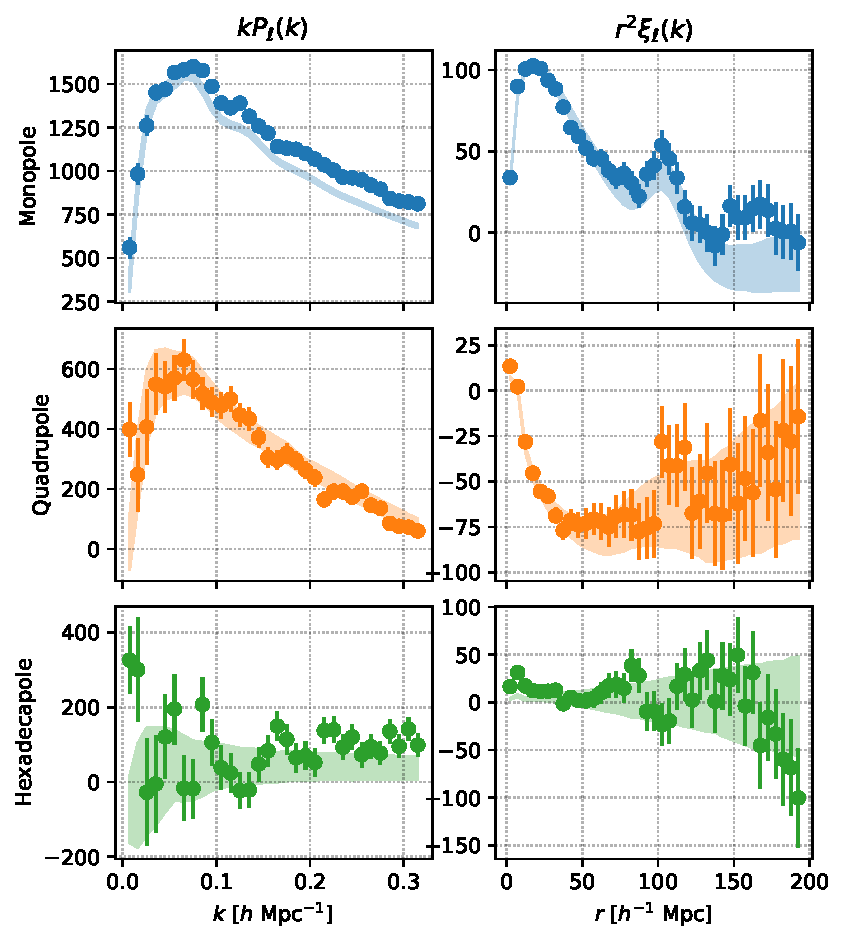
\includegraphics[width=0.8\textwidth]{fig/galaxies/DR16LRG_data_ezmock_prerecon.pdf}
    \caption{Pre-reconstruction multipoles of the two-point statistics for the combination of BOSS DR12 and 
    eBOSS DR16 luminous red galaxies. Left panels contain the power spectrum multipoles (scaled by $k$) 
    and right panels the correlation function multipoles (scaled by $r^2$). 
    Points with errorbars are real data while shaded regions show the mean and standard deviation 
    of 1000 realisations of \textsc{EZmocks}. 
    }
    \label{fig:LRG_data_ezmock_correlations_prerec}
\end{figure}

\begin{figure}
    \centering
    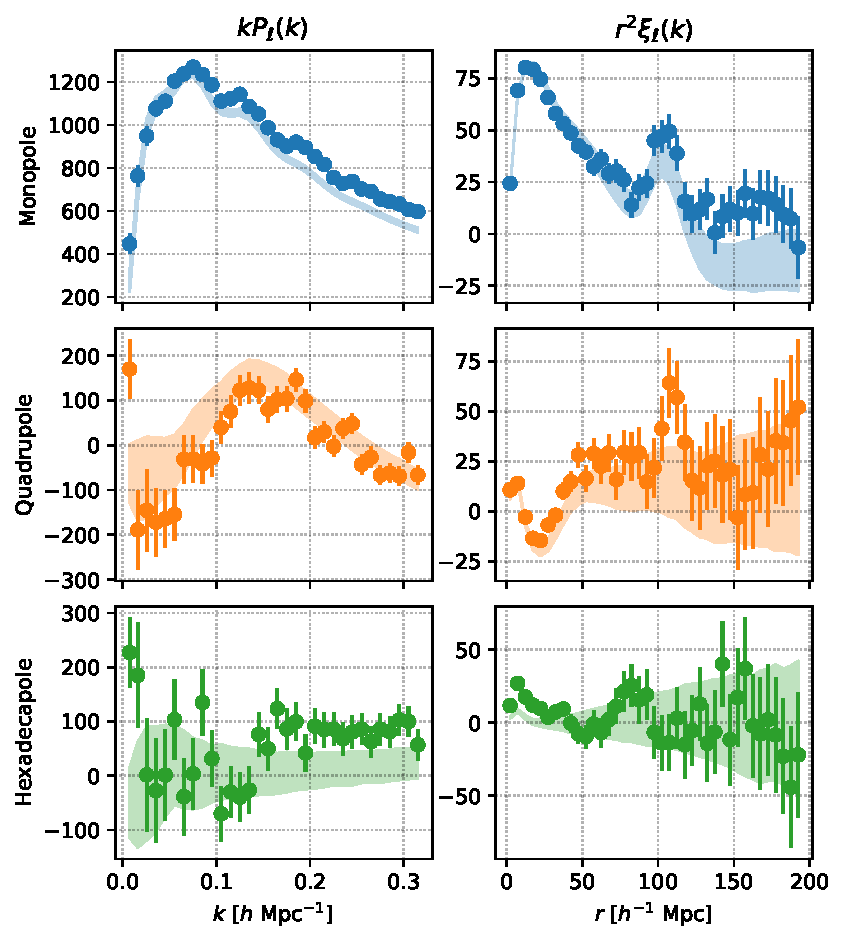
\includegraphics[width=0.8\textwidth]{fig/galaxies/DR16LRG_data_ezmock_postrecon.pdf}
    \caption{Same as Figure~\ref{fig:LRG_data_ezmock_correlations_prerec} but for reconstructed 
    catalogues. We used the Zeldovich reconstruction method with removal of redshift-space distortions. 
    The BAO features are more proeminent and the quadrupole is significantly reduced compared 
    to results with the standard catalogues.    
    }
    \label{fig:LRG_data_ezmock_correlations_postrec}
\end{figure}

The uncertainties on our measurements of $P_\ell$ and $\xi_\ell$ were derived by measuring the 
same statistics on the full sample of 1000 realisations of \textsc{EZmocks}. By reproducing with 
high fidelity the observational features and systematic effects, the covariance matrix obtained 
with mocks should account for the extra scatter induced by them. However on small scales the 
clustering of the mocks is not accurate compared to real data or to more realistic n-body simulations. 
Figure~\ref{fig:covariance_ezmock} shows the resulting covariance matrices normalised by the 
diagonal elements (correlation coefficients). We see how power spectra multipoles are generally 
less correlated than correlation function multipoles. Reconstruction also helps reducing these 
correlations. Also shown are the cross-covariance between Fourier space and configuration space 
measurements, which will be discussed in section~\ref{galaxies:joint}. As expected, these
two spaces are highly correlated since they originate from the same sample of galaxies and randoms. 

\begin{figure}
    \centering 
    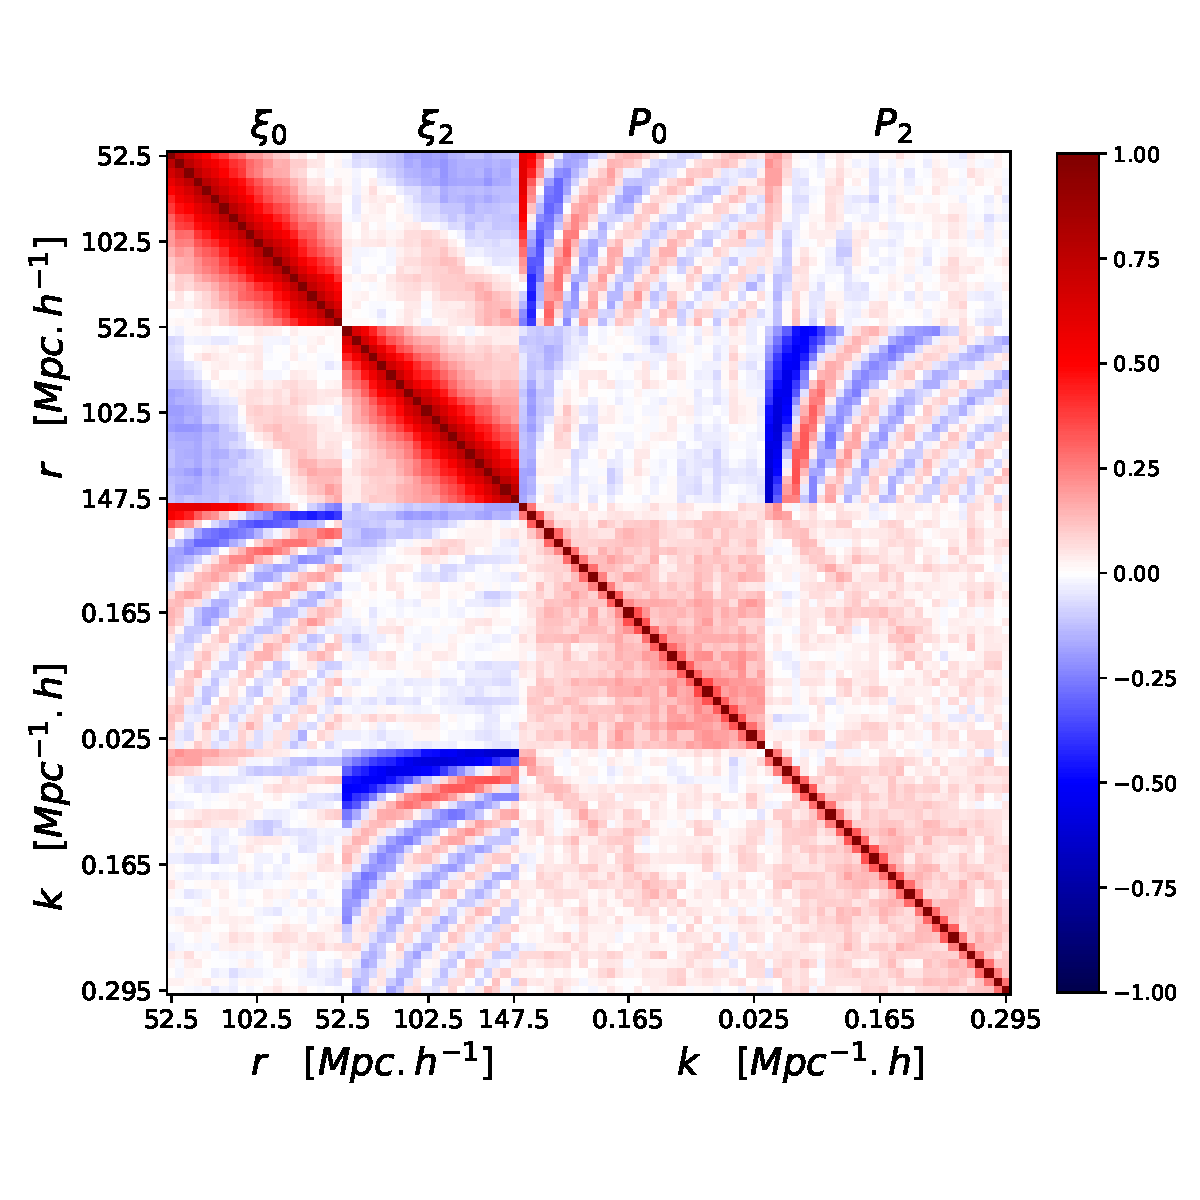
\includegraphics[width=0.49\textwidth]{fig/galaxies/covariance_prerecon.pdf}
    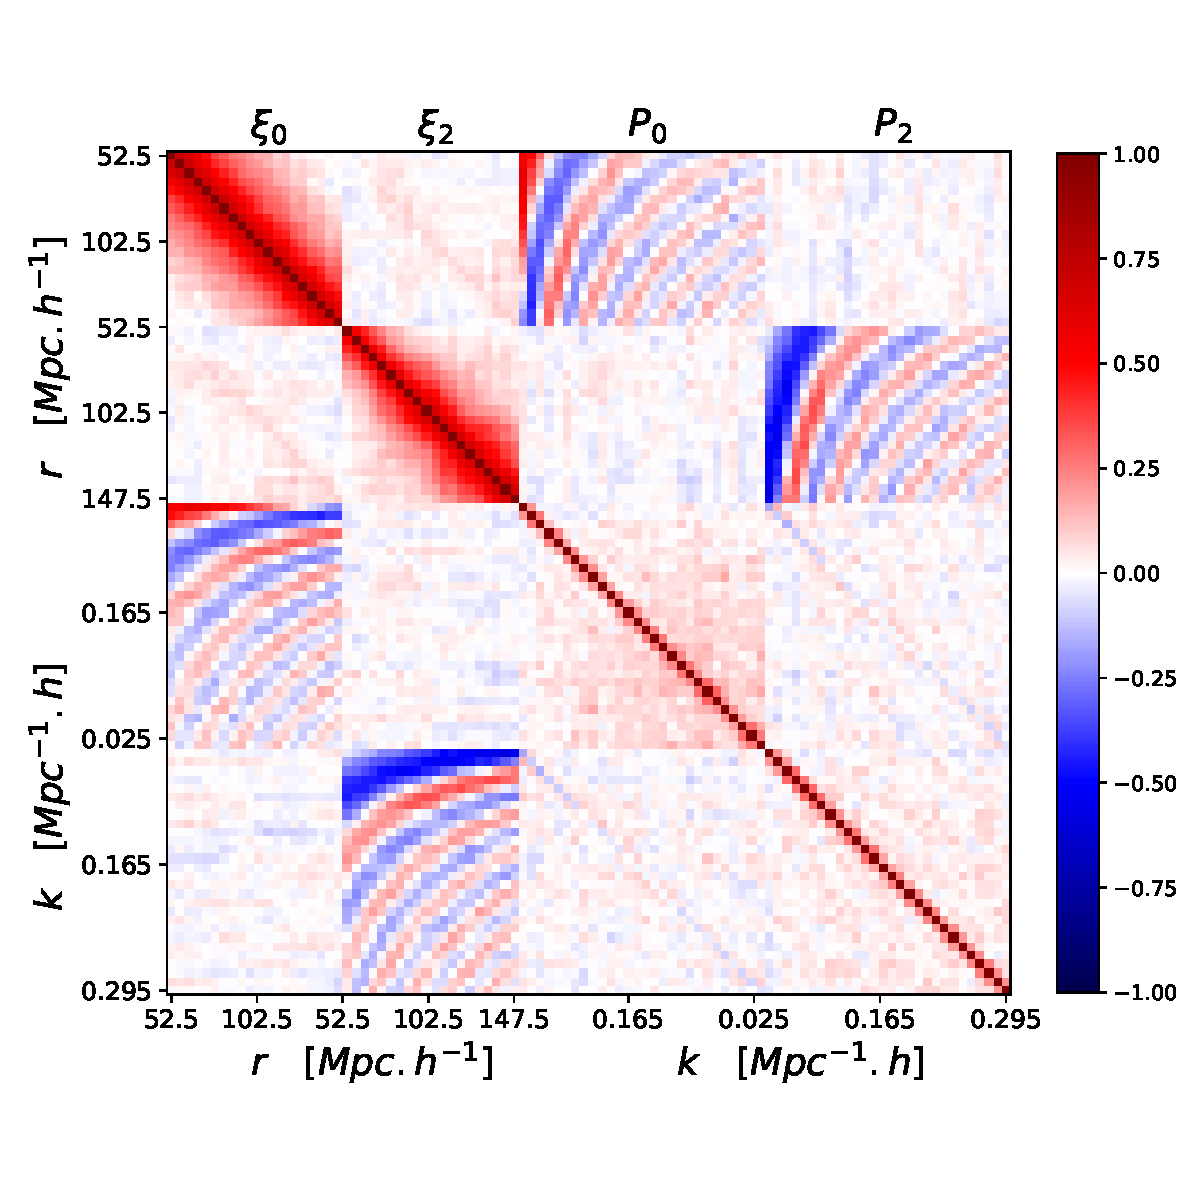
\includegraphics[width=0.49\textwidth]{fig/galaxies/covariance.pdf}
    \caption{Correlation coefficients from covariance matrices obtained from 1000 measurements
    of power spectrum and correlation function multipoles, $P_\ell$ and $\xi_\ell$ respectively,
    from \textsc{EZmocks} reproducing the combined BOSS DR12 and eBOSS DR16 LRG sample.
    Left panel shows results from the standard catalogues while the right panel 
    shows the results from Zeldovich reconstructed catalogues. 
    }
    \label{fig:covariance_ezmock}
\end{figure}

\section{Baryon acoustic oscillations}
\label{galaxies:bao}

Model 

Constraints with DR16 

\section{Redshift-space distortions}
\label{galaxies:rsd}

Model 

Constraints with DR16 

\section{Joint clustering analysis in Fourier and Configuration space}
\label{galaxies:joint}




\section{Cross-correlation with radio surveys}
\label{galaxies:radio}

\cite{wolzHIConstraintsCrosscorrelation2021}

	\chapter{ The low-redshift Universe and its velocities }
	\label{chap:velocities}
	\chaptertoc{}

\vspace{1em}


At low redshifts, peculiar velocities of galaxies can be directly measured 
and be used to learn about gravity on large scales. 
As presented in chapters~\ref{chap:intro} and \ref{chap:galaxies}, velocities 
are generally not observable other than by their indirect impact on the 
galaxy clustering through redshift-space distortions (RSD).
At $z<0.2$, the volume that can be probed by galaxy surveys is insufficient to obtain 
precise measurements of the growth-rate of structures $f$ solely with RSD. 
The additional information from peculiar velocities
significantly improves these constraints, to the point where one 
can perform consistency tests of the standard cosmological model or of our current 
model for gravity: general relativity. 

In this chapter I will expose the recent work we developed within the 
cosmology group at the Centre de Physique des Particules de Marseille 
in trying to combine galaxy surveys and peculiar velocities, 
particularly those obtained from type-Ia supernovae.




\section{Measuring peculiar velocities}
\label{velocities:measuring}

As discussed in section~\ref{intro:probes:rsd}, 
redshifts of galaxies can be seen as a mixture of two distinct types of redshift. 
The first one is due to the expansion of the Universe and we refer to it as 
\emph{cosmological redshift} $z_\text{cos}$. The second one is due to Doppler effect and the peculiar 
velocities of galaxies with respect to a comoving frame, we refer to it as \emph{peculiar redshift} $z_\text{pec}$.
The total observed redshift $z_\text{obs}$ can be written as: 
\begin{equation}
    1+ z_\text{obs} = (1+z_\text{cos})(1+z_\text{pec})
\end{equation}

Measuring peculiar velocities or redshifts $z_\text{pec}$ means 
breaking the degeneracy between $z_\text{cos}$ and $z_\text{obs}$. 
The observed redshift of a given galaxy can be precisely measured via spectroscopy 
but its cosmological redshift requires a measurement of its distance or age, 
of which we can derive $z_\text{cos}$ through a cosmological model.
Therefore, peculiar velocity surveys can be seen simply as distance surveys.

Measuring distance of individual objects on cosmological scales is quite challenging
since it commonly involves standard or standardisable candles. 
For cosmological distances, three types of standardisable candles have been used by
peculiar velocity surveys: spiral galaxies, elliptical galaxies and type-Ia supernovae. 
Many decades of studies of galaxies have pointed to interesting correlations 
between their luminosity or absolute magnitudes, which are not directly observable,
to properties or physical quantities that can be directly observed and do not depend on 
the galaxy distance. 
Two famous correlations are the Tully-Fisher (TF) relation for spiral galaxies 
and the Fundamental Plane (FP) for ellipticals, which we will describe shortly after. 
Needless to say, type-Ia supernovae (SNIa) have been proven to be excellent standardisable candles
when accounting for correlations between their luminosity and the duration and colour of their light-curves. 
As discussed in section~\ref{intro:probes:snia}, SNIa are by themselves a key cosmological probe of 
the Universe's expansion. 

The precision of distance measurements is highly dependent on the modelling of correlations 
between luminosity, from which we derive luminosity distances, and their observed properties. 
Even after standardisation, each method remains with some intrinsic scatter in distances. 
For instance, TF and FP distances have generally a scatter of about 20\% while SNIa 
can reduce it to about 8\%. For cosmological applications, one SNIa distance is worth 4 to 5 
TF or FP distances to obtain the same precision. 
 

    \subsection{The Tully-Fisher relation of spiral galaxies} 
    \label{velocities:measuring:tf}
    
    The Tully-Fisher relation is an empirical link between the mass of spiral galaxies 
    and their rotational velocity at the regime where it does not vary much with distance to 
    the center. \cite{tullyNewMethodDetermining1977} where the first to find a correlation 
    between a distance-independent observable, the asymptotic rotational velocity, and 
    mass or luminosity, and to use it as a method to infer galaxy distances. 
    The physical origin of the relation is the virial theorem of a collapsed object. 

    Later works found that the infrared luminosity correlates better with rotational 
    velocity, i.e., it reduces the remaining scatter. This is because infrared wavelengths 
    are less sensitive to dust extinction than optical wavelengths.  
    \cite{mcgaughBaryonicTullyFisherRelation2000} have later shown that the standard 
    Tully-Fisher relation breaks down for galaxies with small rotation velocities. 
    However, those galaxies contain relatively more gas than stars. If the total baryonic mass 
    is used instead of only stellar mass, the relation holds even for these smaller galaxies. 
    This is known today as the baryonic Tully-Fisher (BTF) relation. 

    One of the largest samples of BTF distance measurements to date is the one provided by 
    the fourth version of the Cosmicflows project (\cite{kourkchiCosmicflows4BaryonicTullyFisher2022}), 
    containing about 10~000 distances. 
    Figure~\ref{fig:pv_footprint} and \ref{fig:pv_zdistrib} show the angular and redshift distribution 
    of this catalogue. 
    The BTF relation of the sample is calibrated using a set of 600 galaxies in 20 well known clusters.
    They used information from HI fluxes from several radio telescopes. The HI fluxes are better 
    tracer of the gas content of the galaxies and the HI line width is related to the rotation 
    velocity of these galaxies. For stellar masses, they used photometry from SDSS in optical 
    and the WISE satellite in the infrared. 
    The infered scatter in their TF relation is of about 45\% in the distance modulus (or absolute magnitudes) 
    which corresponds to a scatter of $\ln(10)/5 \times 45$\%$ = 18$\% in distances.  
    Their sample extends up to $z \sim 0.05$. 
    \cite{hoffmanCosmicflowsDistanceModuli2021} describes how to compute peculiar velocites 
    from this sample of TF distances, including a correct treatment of uncertainties. 

    In section~\ref{velocities:methods} I will present some of the growth-rate measuements 
    using this or a previous version of the CosmicFlows catalogue of distances. 


    \begin{figure}
        \centering 
        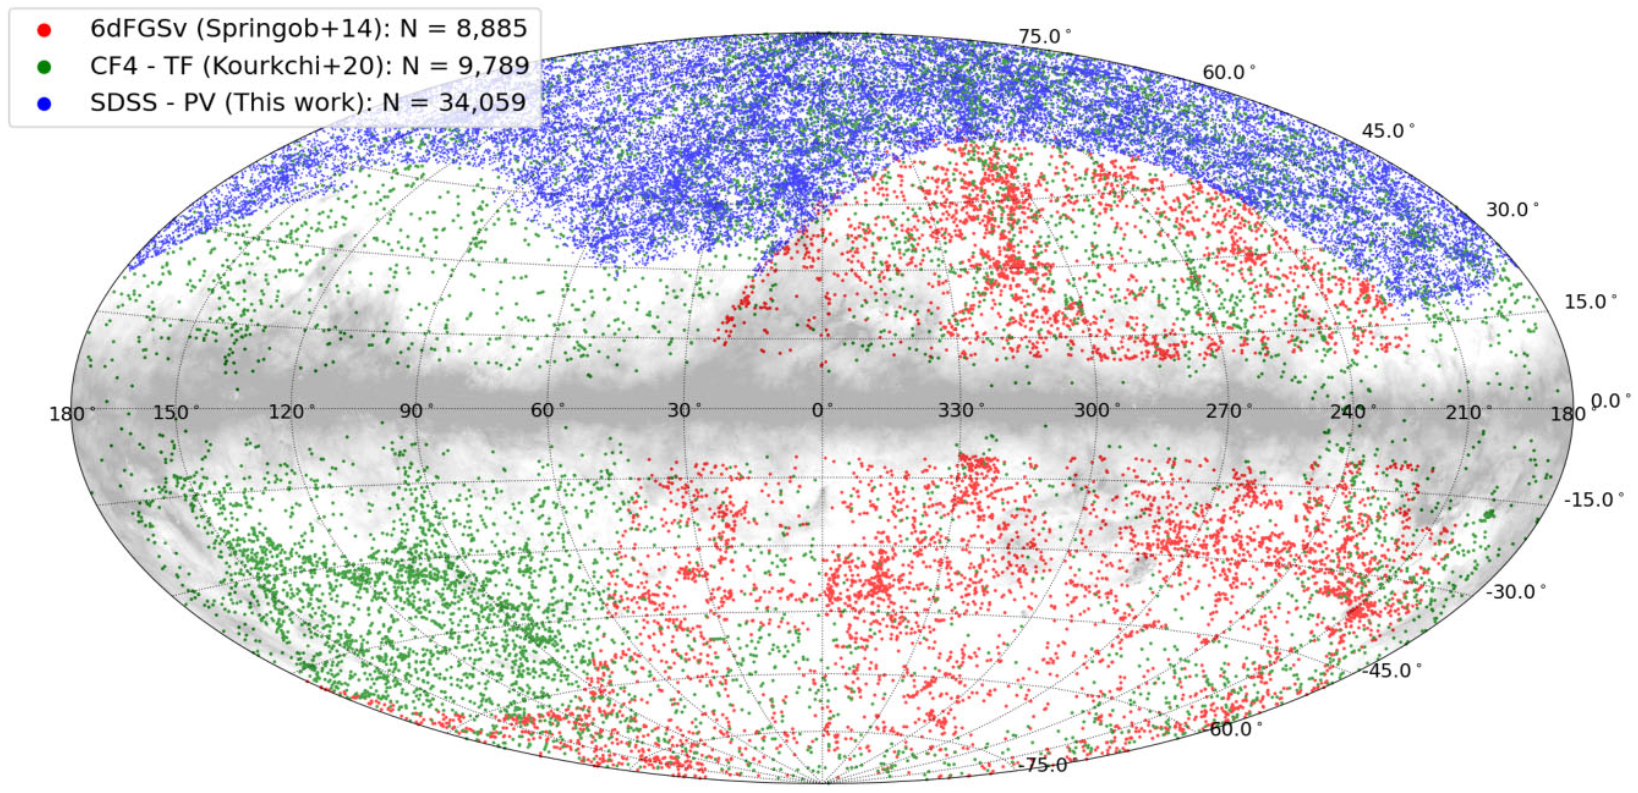
\includegraphics[width=\textwidth]{fig/velocities/pv_footprints.png}
        \caption{Angular distribution of peculiar velocity samples in Galactic coordinates:
        SDSS (blue) and 6dFGSv (red) from Fundamental Plane and 
        Cosmicflows-4 (green) from Tully-Fisher relation.  
        Figure extracted from \cite{howlettSloanDigitalSky2022a}. }
        \label{fig:pv_footprint}
    \end{figure}

    \subsection{The Fundamental Plane of elliptical galaxies} 
    \label{velocities:measuring:fp}
    
    The equivalent of the Tully-Fisher relation for elliptical galaxies is 
    named the Fundamental Plane (FP, \cite{djorgovskiFundamentalPropertiesElliptical1987}). 
    It is an extension in two-dimensions of a previously thought-to-be one-dimensional 
    relation between the luminosity of the elliptical galaxy and 
    the velocity dispersion of their stars near their centres. The one-dimensional version is 
    known as the Faber-Jackson relation (\cite{faberVelocityDispersionsMasstolight1976}). 
    Later, this relation was extended to two-dimenstions to relate the effective radius of the galaxy 
    (in kpc) to the velocity dispersion and the average surface brightness within the effective angular radius. 
    The last two quantities are distance-independent and can be observed with speectroscopy and photometry 
    respectively. From these, we can derive the effective radius which is then converted to a distance measurement. 

    The largest sample of FP distances to date is the one produced from the SDSS project 
    (\cite{howlettSloanDigitalSky2022a}) containing about 34~000 distances. 
    This sample recently surpassed the previous larger sample from the 6-degree Field Galaxy Survey 
    peculiar velocity sample (6dFGSv, \cite{springob6dFGalaxySurvey2014}) which contained nearly 9~000 distances. 
    Figure~\ref{fig:pv_footprint} and \ref{fig:pv_zdistrib} show the angular and redshift distribution 
    of these two catalogues, respectively. 
    The final estimated scatter of the SDSS sample is about 50\% in distance moduli 
    which corresponds to about 23\% in distances, which is similar to the scatter of 
    TF distances. 

    In section~\ref{velocities:methods} I will present some of the growth-rate measuements 
    using the 6dFGSv sample of distances. Currently there are no published results using 
    the larger SDSS sample. 

    \begin{figure} 
        \centering 
        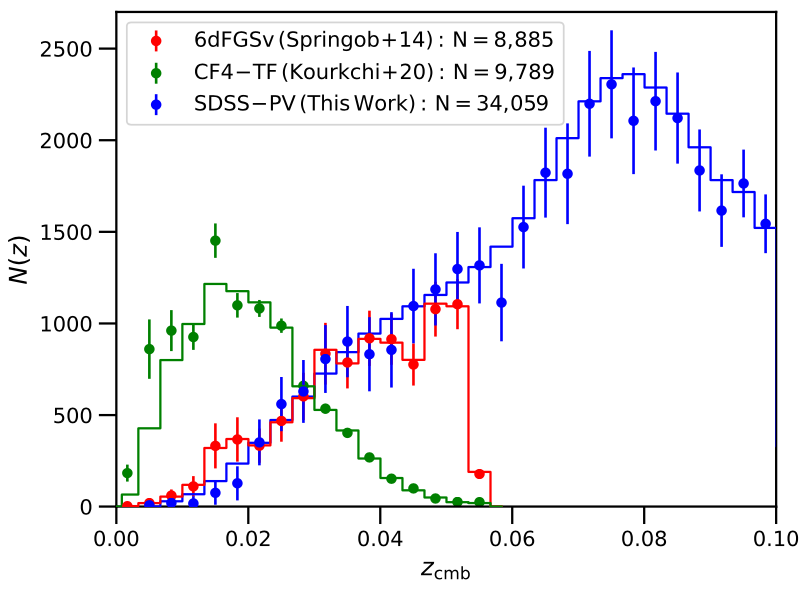
\includegraphics[width=0.5\textwidth]{fig/velocities/pv_zdistrib.png}
        \caption{The redshift distribution of the distance samples: 
        SDSS (blue) and 6dFGSv (red) from Fundamental Plane and 
        Cosmicflows-4 (green) from Tully-Fisher relation. 
        Points with error bars show the number of galaxies per bin of width 1000\kms, 
        where error bars include cosmic variance computed from mock catalogues.
        Solid lines are the mean redshift distributions from these mocks.
        Figure extracted from \cite{howlettSloanDigitalSky2022a}. }
        \label{fig:pv_zdistrib}
    \end{figure}




    \subsection{Type-Ia supernovae}
    \label{velocities:measuring:snia}

    As mentioned earlier, type-Ia supernovae (SNIa) have been used as distance indicators 
    to measure the Hubble constant and the equation of state of dark energy. 
    The state of the art results based on SNIa cover up to redshifts of 2. 

    Since SNIa provide distances, one can also estimate peculiar velocities by 
    looking at the residuals with respect to the best-fit Hubble diagram. 
    Peculiar velocities modifies mostly the observed redshifts than the 
    observed magnitude. Magnitudes are only affected by the relativistic 
    beaming, which scales luminosity distances as $(1+z_\text{pec})^2$, 
    so it is a second-order effect. 
    Figure~\ref{fig:pv_hubble_diagram_snia} sketches how peculiar velocities 
    would impact an ideal case of a SNIa Hubble Diagram without any kind of 
    scatter. We can see how displacements are majoritarily along the redshift direction. 


    \begin{figure}
        \centering 
        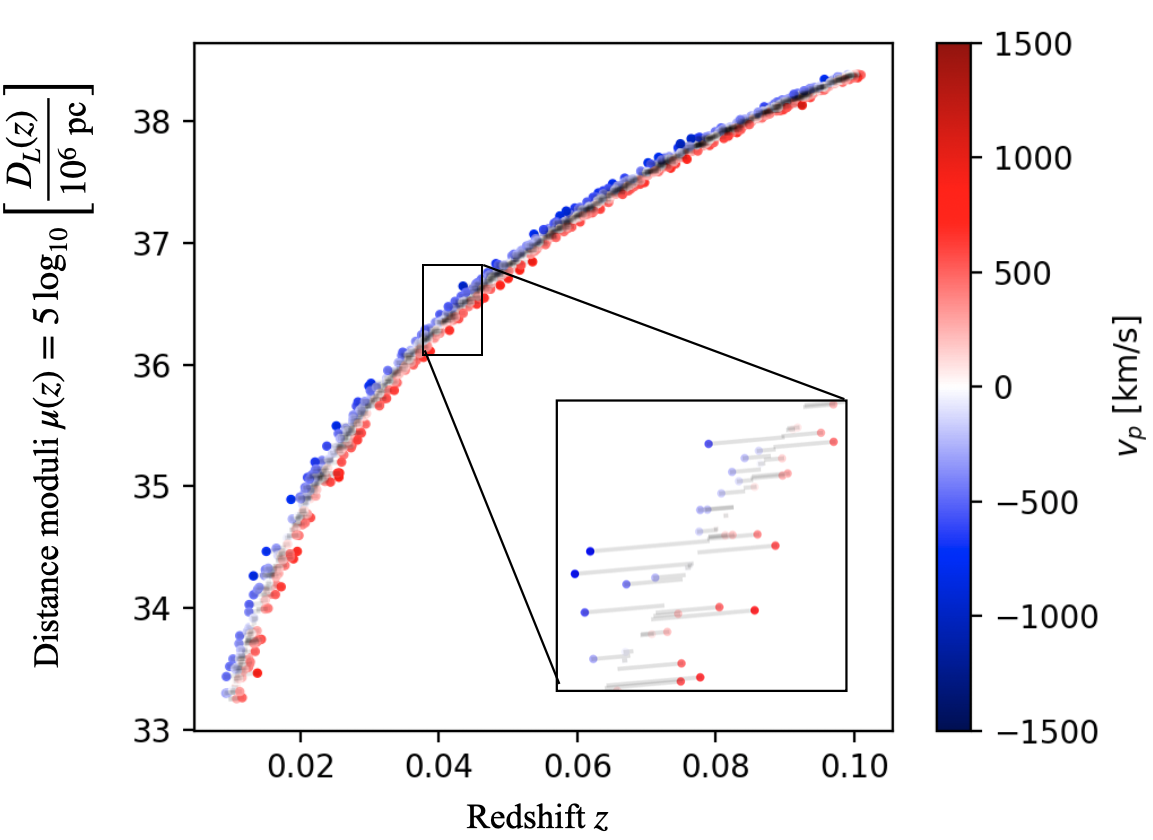
\includegraphics[width=0.7\textwidth]{fig/velocities/pv_hubble_diagram_snia.png}
        \caption{Effect of peculiar velocities on an ideal case of a Hubble Diagram of 
        type-Ia supernovae without any intrinsic scatter or observational uncertainties.
        The displacements along the redshift direction are proportional to $(1+z_\text{pec})$
        while those along the distance moduli direction are proportional to $\log_{10}(1+z_\text{pec})$.
        The colourbar indicates the simulated peculiar velocity of each SNIa. }
        \label{fig:pv_hubble_diagram_snia}
    \end{figure}

    Until now, peculiar velocities were mostly treated as nuisance when 
    constructing the Hubble Diagram. 
    \cite{petersonPantheonAnalysisEvaluating2021} 
    attempted to correct for peculiar velocities of some SNIa of the Pantheon+ sample 
    (\cite{scolnicPantheonAnalysisFull2021}) by using reconstruction techniques on 
    galaxy survey data and by identifying groups of galaxies. 
    Peculiar velocities from SNIa have not been widely used to measure growth-rate for two main 
    reasons. First, the small number of detected SNIa at low redshifts, where uncertainties in 
    velocities are not prohibitive. Second, the inhomogeneity in the available samples which 
    originate from several telescopes, cameras, each with its own observing strategy or 
    prior selection of targets. As we will discuss later, selection effects are important 
    when constructing velocity fields with any type of distance tracer. 
    
    The Zwicky Transient Facitily (ZTF, \cite{grahamZwickyTransientFacility2019}) 
    is currently observing the whole available sky from the Northern 
    hemisphere and will produce a large sample of abouth 5~000 SNIa at $z<0.1$ without any prior 
    selection. This will be a homogeneous set ideal to perform statistical measurements with their 
    peculiar velocities.
    Figure~\ref{fig:pantheon_ztf_sky} compares the angular distribution of SNIa of the Pantheon+ sample 
    to the ZTF Year 1 sample.  
    Figure~\ref{fig:pantheon_ztf_redshift} compares the redshift distribution of the same samples. 
    In section~\ref{velocities:desi_ztf}, I will present the plan of the project of measuring 
    the clustering of ZTF peculiar velocities in combination with galaxies from DESI. 
    
    \begin{figure} 
        \centering 
        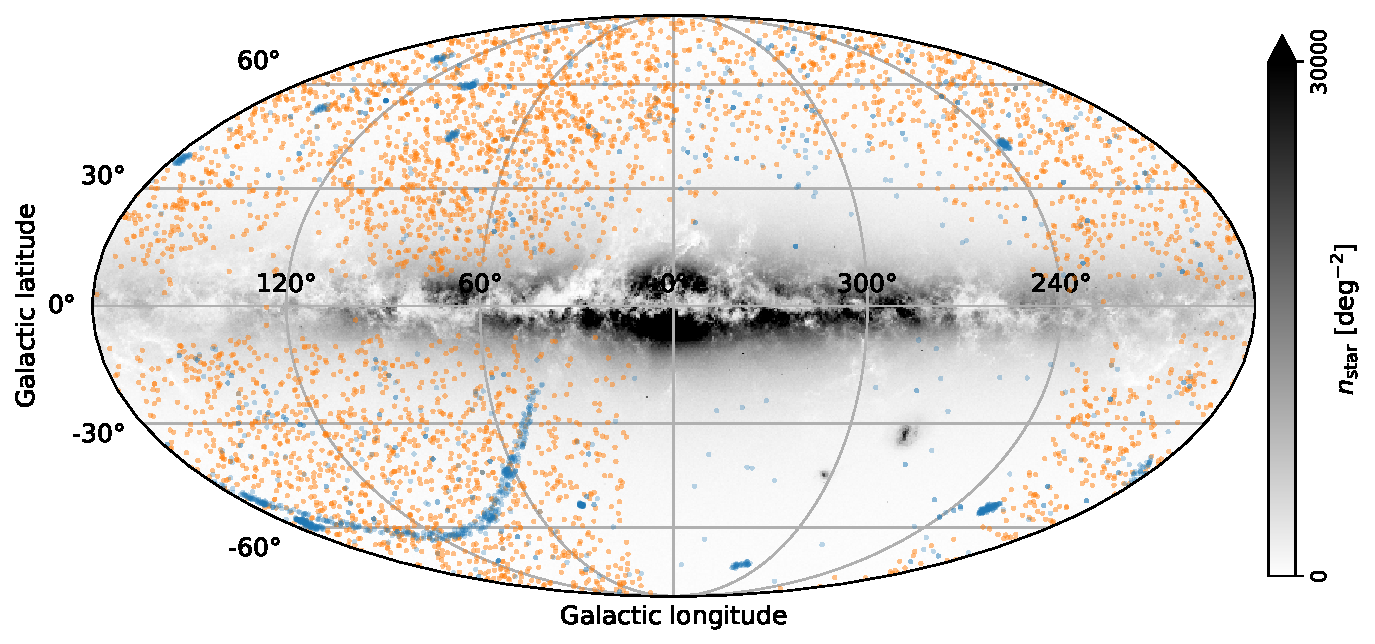
\includegraphics[width=\textwidth]{fig/velocities/ztf_pantheon_gaia.pdf}
        \caption{Angular distribution of type-Ia supernovae in Galactic coordinates
        for the Pantheon+ sample (blue) and for ZTF Year 2 sample (orange). 
        On the background we see the stellar density distribution from Gaia. 
        }
        \label{fig:pantheon_ztf_sky}
    \end{figure}

    \begin{figure} 
        \centering 
        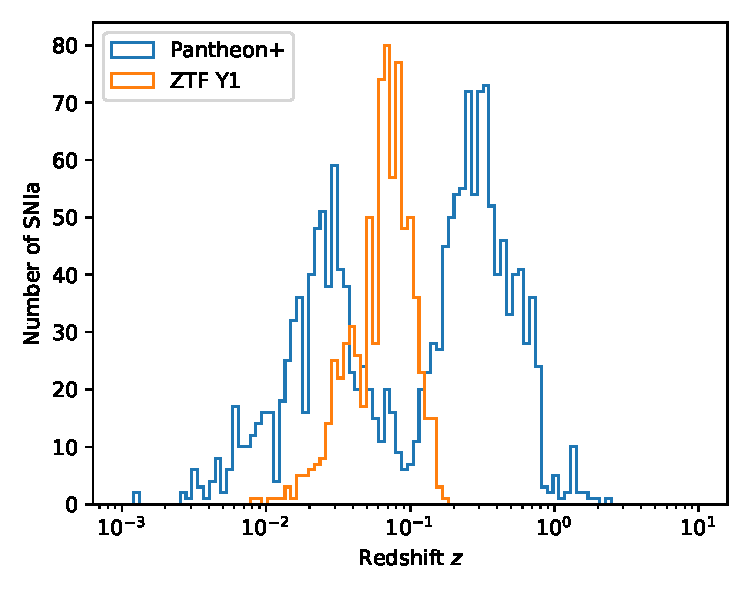
\includegraphics[width=0.6\textwidth]{fig/velocities/nz_ztfy1_pantheon.pdf}
        \caption{Redshift distribution of host galaxies of type-Ia supernovae 
        for the Pantheon+ sample (blue) and for ZTF Year 1 sample (orange).
        }
        \label{fig:pantheon_ztf_redshift}
    \end{figure}

\section{Biases affecting velocities}
\label{velocities:biases}

One of the main difficulties with distance measurements based on standardisable candles 
and their statistical properties (see next section) is the impact of certain types of biases. 
The review by \cite{straussDensityPeculiarVelocity1995} discuss all these biases and how they  
impact clustering analyses. They can be classified in three types: selection bias, homogeneous 
and inhomogeneous Malmquist biases. The term Malmquist is often used to refer to selection bias,
but I will follow the convention of \cite{straussDensityPeculiarVelocity1995}. 

The selection bias, as the name indicates, is caused by some selection or detection criteria 
on the sample of objects. For instance, it is pretty common to impose some cuts on signal-to-noise 
ratio of fluxes or some magnitude limit. For objects close to the boundary, only 
the brighter objects pass the cuts. If one is interested in, say, the average distance of these objects, 
we will observe a bias relative to the true average distance. 
The intrinsic scatter in luminosity of all standardisable candles worsens this type of bias 
and it complicates any attempts to correct for these biases. 
Typical analyses of SNIa ofter use realistic simulations of the data, including the physical 
properties of SNIa that create the scatter and instrumental noise, to model these selection effects. 
The analysis of the Panthon SNIa sample used a technique named 
Bayesian Estimation Applied to Multiple Species (BEAMS, \cite{kunzBayesianEstimationApplied2007}) 
with Bias Corrections 
(BBC, \cite{kesslerCorrectingTypeIa2017}). This technique also accounts for mis-classified supernovae. 

The homogeneous Malmquist bias manifests itself due to the fact that the number of objects 
observed as a function of distance to us increases with distance squared. When averaging 
objects in a given distance or redshift range, they are not uniformly distributed inside this range,
so the average distance is higher than the true distance, often assigned to the center of the range. 
Is this true ? Check! 
 
The inhomogeneous Malmquist bias is a similar effect but generalised to the fluctuations in density 
(due to structures) along the line of sight. This bias depends on the precise shape of $\delta(\hat{n}, d)$
where $\hat{n}$ is a given direction in the sky and $d$ is the distance to us. 

It is possible to correctly account for all these biases in a fully Bayesian treatment of  
propability density functions of the distances 
(\cite{grazianiPeculiarVelocityField2019, boruahReconstructingDarkMatter2021}). 

\section{Growth-rate measurements with velocities}
\label{velocities:methods}


With a set of distance or peculiar velocity measurements, 
we can study them statistically and compare to predictions from 
cosmological models, just as we did with the overdensities of fluxes 
in chapter~\ref{chap:forests} or galaxies in chapter~\ref{chap:galaxies}. 

One can see this additional set of observables as a scalar field, the radial 
velocity field  $v_r(\vec{x}_i)$, sampled 
at the positions of the galaxies from which they were measured $\vec{x}_i$, 
where $i=1,\ldots,N_\text{gal}$. 
Instead of radial velocities, it is quite common to use the log of the ratio between the distance inferred from 
the redshift and the distance inferred from the luminosity, called log-distance ratio. 
Log-distance ratios have uncertainties that can be approximated by a Gaussian, 
whereas in velocity space the uncertainties become log-normal are harder to handle. 

The first statistic that one can think of measuring is the correlation function of the 
radial velocities  $\xi_{v_r v_r} \equiv \langle v_r(\vec{x}_i) v_r(\vec{x}_j) \rangle$ 
(or the equivalent for log-distance ratios). 
If one has, in addition to the velocities, a galaxy survey over the same volume, one
can use the observed overdensity field $\delta(\vec{x})$ to cross-correlate with the 
observed velocity field, i.e., $\xi_{\delta_g v_r} \equiv \langle \delta(\vec{x}) v_r(\vec{y})\rangle$. 
The auto-correlation of the overdensity field $\xi_{\delta_g \delta_g} \langle \delta(\vec{x})\delta(\vec{y})\rangle$ 
is the equivalent to the one used in BAO and RSD measurements. 
These three statistics can be analysed jointly when comparing to models, 
increasing the constraining power. 

I will shortly describe a few methods available in the litterature that 
allows us to connect models to the obseved densities and velocities, 
at the field level or at the two-point function level. 

    \subsection{Maximum likelihood method}
    \label{velocities:methods:maximum_likelihood}

    The idea is to maximise the likelihood, assumed to be a multivariate Gaussian on 
    the velocities,
    \begin{equation}
        \mathcal{L}(\vec{p}) = \frac{1}{(2 \pi)^{\frac{n}{2}} \text{det}[C(\vec{p})]^{1/2} }
            \exp\left[-\frac{1}{2} v_r^T C(\vec{p})^{-1} v_r\right]
        \label{eq:likelihood}
    \end{equation}

    with respect to a set of parameters $\vec{p}$. Here $v_r$ is a vector containing each 
    measured peculiar velocity and the covariance matrix $C(\vec{p})$ is the model 
    for the two-point statistics of $v_r$. Each element of the covariance is given by 
    $C_{ij} =  \xi^\text{model}_{v_r v_r}(\vec{x}_i, \vec{x}_j, \vec{p}) + \delta^K_{ij} \sigma_i \sigma_j$, 
    where $\sigma_i$ is a diagonal noise term, often accounting for instrumental uncertainties 
    as well as intrinsic scatter of distance measurements. 
    The first term in the covariance 
    is the cosmic variance and it is connected to a cosmological model. 

    The cosmological part of the covariance $C_{ij}$ is often written as a 
    Fourier transform of the two-point statistics in Fourier space, 
    often described by the velocity or the velocity-divergence power 
    spectrum. 
    Most of previous works have used linear perturbation theory with  
    some empirical terms that account for non-linearities.  
    In linear theory, the velocity field $\vec{v}(\vec{x})$ is irrotational, meaning it 
    is completely defined as the gradient of a scalar field $\theta(\vec{x})$. 
    This velocity divergence is equal to the overdensity of matter $\delta(\vec{x})$ for linear perturbations. 
    Therefore the two-point statistics of the velocity is proportional to the linear matter power spectrum 
    (and thus to $\sigma^2_8$) and to the linear growth-rate of structures $f$. 

    The maximum likelihood method has been used on several peculiar velocity samples
    such as the 6dFGSv (\cite{campbell6dFGalaxySurvey2014, springob6dFGalaxySurvey2014})
    with velocities alone (\cite{johnson6dFGalaxySurvey2014}), in combination with density field 
    (\cite{adamsImprovingConstraintsGrowth2017, adamsJointGrowthrateMeasurements2020}), 
    or adding a few SNIa (\cite{hutererTestingLCDMLowest2017}). 
    
    At CPPM, Bastien Carreres is currently employing this technique to analyse 
    the ZTF sample of type-Ia supernovae. I have implemented the basic algorithm 
    and Bastien continued its development, adapting it to work with log-distance 
    ratio instead of velocities, several mesh assignement schemes and models of clustering. 
    He also implemented a whole pipeline to produce realistic simulations of ZTF SNIa light-curves, 
    which can be painted on n-body simulations, and to analyse them as real data. 
    He is currently studying 
    the impact of selection biases on the estimates of $f\sigma_8$ using the 
    maximum likelihood method. First results on simulated data show that an unbiased measurement 
    is possible if we limit our analysis to SNIa at $z< 0.05$. 
    We will apply our methodology to real data once the final ZTF SNIa is set. 


    \subsection{Compressed two-point statistics}
    \label{velocities:methods:compressed_two_point} 

    The compression of two-point statistics means that we combine measurements 
    into separation or wavenumber bins, depending if we are in configuration or Fourier space. 
    Estimating compressed statistics is the most common method for  
    standard clustering analysis, as we saw in earlier chapters, 
    where we aim to estimate the correlation function or the power spectrum.
    The modelling happens at the compressed statistics level, so there are generally less 
    degrees of freedom than for the maximum likelihood method. 

    In configuration space, the velocity auto correlation cannot simply be written as 
    a unique function of separation $\vec{r}$ between two galaxies, since velocities are 
    a vector field. \cite{gorskiPatternPerturbationsHubble1988} introduced the 
    correlation tensor defined as 
    \begin{equation}
        \Psi_{i, j}(\vec{r}_A, \vec{r}_B) \equiv \langle v_i(\vec{r}_A) v_j(\vec{r}_B) \rangle 
        \label{eq:correlation_tensor}
    \end{equation}
    where $i, j$ denote each component of the peculiar velocity field $\vec{v}$. 
    If the field is irrotational, homogeneous and isotropic, the correlation tensor 
    can be written as 
    \begin{equation}
        \Psi_{i, j}(\vec{r}) = 
        \left[ \Psi_\parallel(r) - \Psi_\perp(r) \right] \hat{r}_{Ai} \hat{r}_{Bj} 
        + \Psi_\perp(r) \delta^K_{ij}
    \end{equation}
    where $\Psi_\parallel(r)$ and $\Psi_\perp(r)$ are functions describing the correlations 
    the components of the peculiar velocities parallel and perpendicular to the 
    separation vector $\vec{r}$. Both functions can be written as transforms of the linear 
    matter power spectrum. 

    The correlations between the radial velocities of two galaxies
    relative to the observer, as depicted in 
    Figure~\ref{fig:pv_config}, can be written as 
    \begin{equation}
        \langle u_A(\vec{x})u_B(\vec{x}+\vec{r}) \rangle = 
        \Psi(r) \cos \theta_{AB} 
        + \left[ \Psi_\parallel(r) - \Psi_\perp(r) \right] \cos \theta_A \cos \theta_B. 
    \end{equation}
    
    

    \begin{figure}
        \centering 
        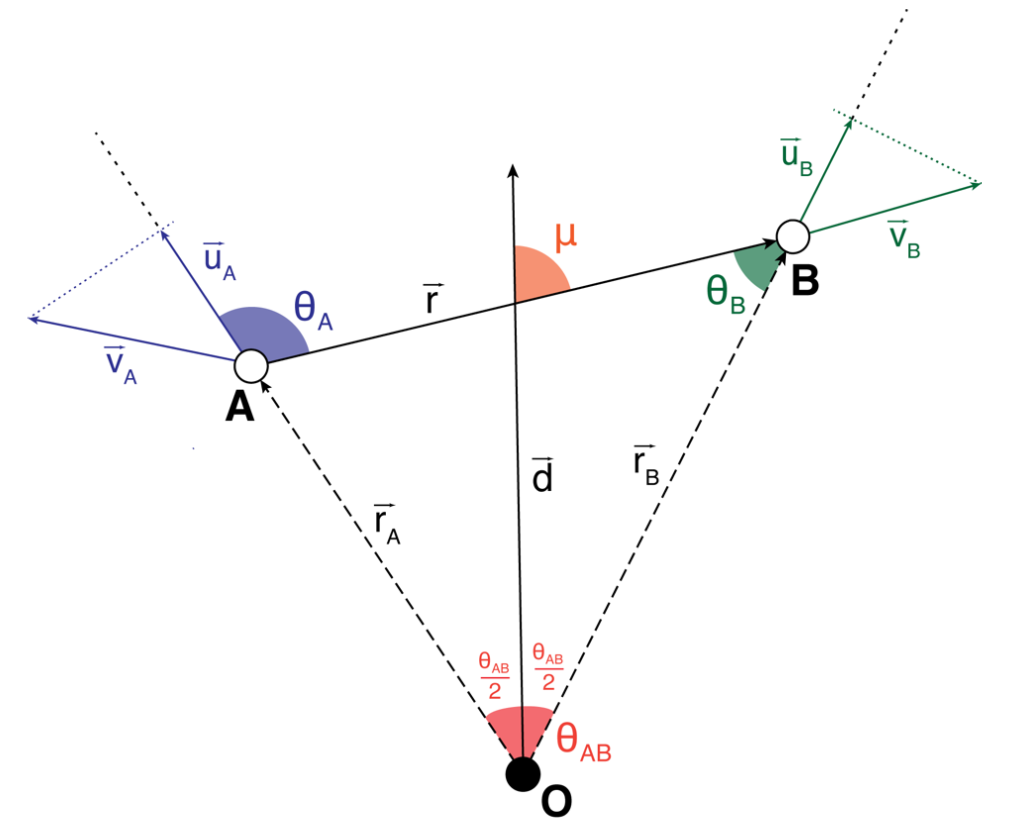
\includegraphics[width=0.6\textwidth]{fig/velocities/pv_config.png}
        \caption{Non-parallel lines-of-sight of a pair of galaxies A and B as seen by an observer O.
        $\vec{r}_A$ and $\vec{r}_B$ are their position vectors, respectively, 
        and $\vec{r}$ is the separation vector between them. 
        The peculiar velocities of galaxies A and B are represented by $\vec{v}_A$ and $\vec{v}_B$, 
        and the radial component of these velocities are represented by $\vec{u}_A$ and $\vec{u}_B$. 
        The pair line-of-sight $\vec{d}$ is defined at the mid-angle and $\mu \equiv \hat{d} \cdot \hat{r}$. 
        Figure extracted from \cite{turnerLocalMeasurementGrowth2022}. 
        }
        \label{fig:pv_config}
    \end{figure}

    \cite{gorskiCosmologicalVelocityCorrelations1989} developed estimators that we can relate to a model that depends on $\Psi_\parallel$ and $\Psi_\perp$. 
    This type of correlation functions were used in 
    \cite{wangPeculiarVelocityCorrelation2018, 
    dupuyEstimationLocalGrowth2019, 
    turnerImprovingEstimatesGrowth2021,
    turnerLocalMeasurementGrowth2022}. 

    In Fourier space, given the sparsity of the data, it is hard to use FFTs on the 
    observed velocity field. This is because voxels without data cannot be assigned 
    zero velocity: the field would be ill-defined there. 
    For this reason, 
    \cite{howlettRedshiftspaceMomentumPower2019} suggests to use the momentum power 
    spectrum, a quantity commonly used in the analysis of velocities in n-body simulations. 
    The momentum is simply the mass-weighted velocity field, written as
    $\vec{p}(\vec{x}) = \left[1+\delta(\vec{x})\right] \vec{v}(\vec{x})$. 
    In the absence of galaxies or velocity measurements, 
    the momentum is well defined and equal to zero. 

    The first application of the momentum power spectrum method was 
    performed by \cite{qinRedshiftspaceMomentumPower2019} on the combined 
    sample of 6dFGSv and the 2MASS Tully-Fisher survey (2MTF). 

    The analysis in compressed statistics is generally faster and more intuitive
    than other methods. The data versus model comparison is commonly easier with 
    compressed statistics. However, one has to be careful when accounting for 
    survey properties, wide-angle effects or redshift evolution. These effects
    are generally easier to deal with in other methods. 


    \subsection{Density-velocity comparison}
    \label{velocities:methods:comparison}

    The link between density and velocity fields is straighforward 
    on quite large scales, where linear theory is valid. 
    Another method to test for the consistency of the standard cosmological model 
    is to compare the observed (radial) velocity field with 
    predictions based on the observed density field. 
    This method is often referred to as density-velocity comparison.  

    Reconstruction techniques discussed in section~\ref{galaxies:reconstruction}
    aim to compute past trajectories of galaxies and therefore their velocities based 
    on the observed density field. Reconstruction yields a prediction for the radial 
    velocities at the locations where we measured them from the distance surveys.
    The inputs are often some value for the large scale bias $b$ of the galaxy sample 
    as well as the growth-rate $f$.  
    Commonly, an empirical amplitude $A$ is fitted to the relation $v_r^\text{obs} = A v_r^\text{model}$. 
    Any deviations from $A=1$ would indicate an inconsistency in the standard 
    cosmological model. From this amplitude, one can quote a value for $f\sigma_8$ 
    if a bias value and a $\sigma_8$ value are assumed.  

    Several applications of this method can be found in he literature. 
    \cite{davisLocalGravityLocal2011} used the Two Micron All-Sky Redshift Survey 
    (2MRS or 2M++ for its extended version) 
    galaxy catalogue as the input for reconstruction and fitted 
    the inverse Tully-Fisher relation to spiral galaxies from the 
    Spiral Field I-band ++ survey (SFI++). 
    \cite{carrickCosmologicalParametersComparison2015} improved the analysis 
    and reported results using the same samples. 
    \cite{boruahCosmicFlowsNearby2020} added peculiar velocities from 465 SNIa 
    to the SFI++ and the 2MTF samples. 
    \cite{saidJointAnalysis6dFGS2020} used a larger dataset of nearly 16k peculiar velocities 
    by combining 6dFGSv and SDSS samples, and compared to the density field from the 2M++. 
    
    At CPPM, Elena Sarpa has a more advanced reconstruction technique 
    called extended Fast Action Minimization (eFAM, \cite{sarpaExtendedFastAction2021})
    which can be readily used to implement the density-velocity comparison.
    The eFAM technique yields higher-order trajectories than 
    Zeldovich reconstruction, which might lead to more realistic 
    predictions for the peculiar velocities. 
    This technique will be potentially applied to the DESI and ZTF data,
    after a detailed comparison with the maximum likelihood method. 


    \subsection{Forward-model of density and velocity field}
    \label{velocities:methods:forward}

    Instead of estimating summary statistics with the density and velocity fields, 
    one can attempt to fit directly the observed fields with some model 
    that depend on cosmological parameters. Typically, the model is composed 
    of some cosmological parameters and a set of initial density and velocity fields
    (one amplitude parameter per mode). These initial conditions are then evolved 
    linearly or using more advanced techniques and then compared to observations. 
    The final product is a posterior on cosmological parameters and on the amplitudes 
    of the initial fields. This method is commonly referred to as \emph{forward-modelling}. 

    In forward modelling, complications due to selection functions are slightly easier 
    to deal with in principle. One has to simulate observations on the evolved fields j
    ust as one does when creating mock catalogues. 
    Also, by modelling the observed field entirely, we capture 
    more information from higher-order statistics than just the two-point function. 
    The inconvience of this method is the computing time required to perform the inference,
    given the large number of free parameters and the time to evolve each sample from initial conditions. 
    
    \cite{lavauxBayesian3DVelocity2016} implemented the forward-modelling applied to 
    both density and velocity fields. A similar approach was used on CosmicFlows3 data 
    by \cite{grazianiPeculiarVelocityField2019}. In \cite{boruahReconstructingDarkMatter2021}
    they discuss the treatment of the inhomogenous Malmquist bias in the Bayesian formalism 
    (see section~\ref{velocities:biases}).
    In \cite{prideaux-gheeFieldBasedPhysicalInference2022}, they used a Bayesian hierarchical modelling 
    approach to fit both density and velocity fields using a Hamiltonian Monte Carlo sampling of the 
    likelihood. 

\section{Current measurements}
\label{velocities:current}

Several measurements were made in the past decade using a variety of distance surveys, 
galaxy surveys and methods. 
Table~\ref{tab:pv_current_measurements} summarises most measurements in the literature.
They are also visually represented in Figure~\ref{fig:pv_current_measurements}. 
All these measurements of the growth-rate $f\sigma_8$ correspond to an effective redshift between zero and 0.1. 
These results are in good agreement with the predictions from a $\Lambda$CDM+GR model, with 
cosmological parameters from \cite{planckcollaborationPlanck2018Results2020}. 
However, one can notice how they do not have the same uncertainties, even if, for some cases, they 
use the same datasets. Few analyses quote systematic uncertainties which can be quite significant for  
some methods. 

The goal of the project I am currently leading at CPPM is to deeply understand those variations 
while optimising the analysis. Also we plan to work closely to the data reduction teams 
in order to produce the best set of simulated data. 
Mock catalogues will be essential to estimate biases 
in best-fit parameters, statistical and systematic uncertainties. 
In the following section I will introduce two datasets that will be used in our project: DESI and ZTF. 

\begin{table}
    \small 
    \centering
    \caption{Measurements of the growth-rate of structures from peculiar velocity 
    and galaxy survey data. }
    \label{tab:pv_current_measurements}
    \begin{tabular}{lllc} 
        \hline 
        \hline 
        Reference  &  Dataset  &  Method   &   $f\sigma_8$  \\ 
        \hline 
%\cite{beutler6dFGalaxySurvey2012a}          & 6dFGSz    & RSD               & $ 0.423 \pm 0.055 $           \\
%\cite{blakePowerSpectrumMultipoles2018}     & 6dFGSz    & RSD               & $ 0.380 \pm 0.120 $ \\
\cite{johnson6dFGalaxySurvey2014}           & 6dFGSv    & Max-likelihood    & $ 0.428^{+0.079}_{-0.068} $   \\
\cite{hutererTestingLCDMLowest2017}         & 6dFGSv    & Max-likelihood    & $ 0.428^{+0.048}_{-0.045} $   \\
\cite{adamsJointGrowthrateMeasurements2020} & 6dFGSz,6dFGSv & Max-likelihood & $ 0.384 \pm 0.052^\text{(stat)} \pm 0.061^\text{(syst)} $ \\  
\cite{laiConstrainingGrowthRate2022}        & SDSS-FP   & Max-likelihood    & $ 0.405^{+0.076 \text{(stat)}}_{-0.071} \pm 0.009^\text{(syst)} $ \\
\cite{qinRedshiftspaceMomentumPower2019}    & 6dFGSv,2MTF & Compressed 2pt  & $ 0.404^{+0.082}_{-0.081} $ \\
\cite{howlett2MTFVIMeasuring2017}           & 2MTF      & Compressed 2pt    & $ 0.510^{+0.090}_{-0.080} $ \\
\cite{nusserVelocitydensityCorrelationsCosmicflows32017} 
                                            & CF3,2MRS  & Compressed 2pt    & $  0.400 \pm 0.080 $ \\ 
\cite{dupuyEstimationLocalGrowth2019}       & CF3       & Compressed 2pt    & $ 0.430 \pm 0.030^\text{obs} \pm 0.110^\text{cosmic} $ \\ 
\cite{davisLocalGravityLocal2011}           & 2MRS,SFI++ & $\delta-v$ comparison & $ 0.310 \pm 0.040 $ \\
\cite{carrickCosmologicalParametersComparison2015} 
                                            & 2MRS,SFI++ & $\delta-v$ comparison & $ 0.401 \pm 0.024 $ \\
\cite{boruahCosmicFlowsNearby2020}          & 2M++,2MTF,SFI++,A2 &  $\delta-v$ comparison & $ 0.400 \pm 0.017 $ \\
\cite{saidJointAnalysis6dFGS2020}           & 2M++,6dFGSv,SDSS-FP & $\delta-v$ comparison & $ 0.311 \pm 0.027 $ \\

        \hline 
        \hline 
    \end{tabular}
\end{table}

\begin{figure}
    \centering 
    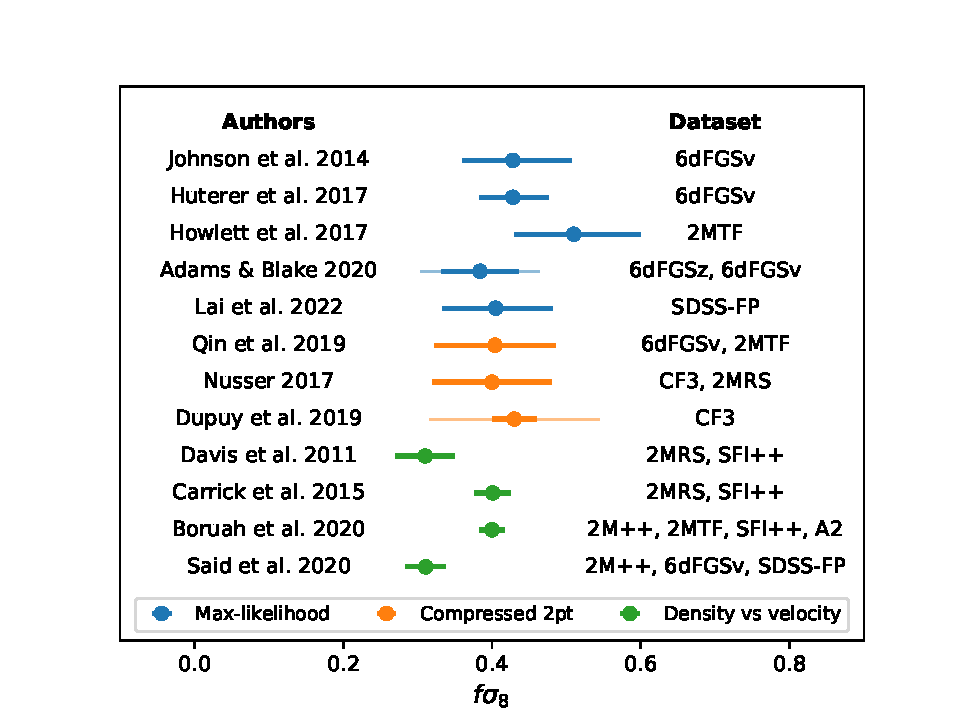
\includegraphics[width=0.8\textwidth]{fig/velocities/plot_fs8_pv.pdf}
    \caption{Measurements of the growth-rate of structures $f\sigma_8$ from peculiar velocity 
    and galaxy survey data. The references and values are listed in Table~\ref{tab:pv_current_measurements}.
    The light error bars include systematic errors. In the case of Dupuy et al. 2019, the extra contribution 
    is from cosmic variance, instead. }
    \label{fig:pv_current_measurements}
\end{figure}

\section{DESI and ZTF}
\label{velocities:desi_ztf}

Both the Dark Energy Spectroscopic Instrument (DESI) and the Zwicky Transient Facility (ZTF)
are currently observing similar area of the sky and building one of the best samples for a joint study of 
densities and peculiar velocities for cosmology. 
One of the main advantages is the great overlap in volume of both surveys. The 14k deg$^2$ footprint 
of DESI will be completely covered bt ZTF observations, which cover up to 18k deg$^2$ of area. 

The main science goal of DESI is to produce precise measurements of the Universe's expansion and 
the growth history of structures, in order to test models of dark energy and gravity. 
DESI will observe more than 20 million galaxies and quasars from up to redshifts of 4.5. 
The bright time of the survey, i.e., when the moon is up, is dedicated to building a flux limited sample of
galaxies at low redshift: the Bright Galaxy Survey (BGS). The BGS will collect roughly 10 million galaxies 
with $r$-band magnitude $r < 19.5$, which lie at $z < 0.6$. 
A fainter  $19.5<r<20.175$ sample will extend and increase the completeness in stellar mass of the BGS sample. 
This sample is not only ideal for BAO and standard RSD measurements, but also for higher order statistical 
measurements, multi-tracer analyses, given its high completeness and simple selection function. 
Most of the ZTF SNIa will have their host-galaxy redshifts measured by the DESI BGS.
It is expected that the BGS observations will complete by 2024 the latest. 

The ZTF survey main goal is to observe the transient sky in three optical bands. 
Most of the sky area is covered every two nights with a given filter, which is excellent cadence 
for discovery and study of SNIa. 
At its current configuration, ZTF is expected to discover around 15k supernovae, 
out of which about 30\% will have spectroscopic classifications. 
The host galaxy redshifts are obtained from archival data, some of which will be observed by DESI 
in the near future. We expect a final sample of 5k cosmology-level spectroscopic SNIa at  
$z < 0.1$. 

Figure~\ref{fig:nz_desi_ztf} compares the density of tracers between DESI BGS and ZTF SNIa, expected at 
the end of their 5-year programs. The density of ZTF SNIa falls quickly after $z \sim 0.06$ where 
selection effects start to kick in. Rough estimates show that the ZTF SNIa sample is \emph{complete},
i.e., all potentially observable SNIa were observed, at $z < 0.05$. 
While the density of ZTF SNIa is several orders of magnitudes lower 
than those of BGS galaxies, the fact that each SNIa yields a measurement of the velocity field 
makes them a powerful tracer nevertheless. 

\begin{figure}
    \centering
    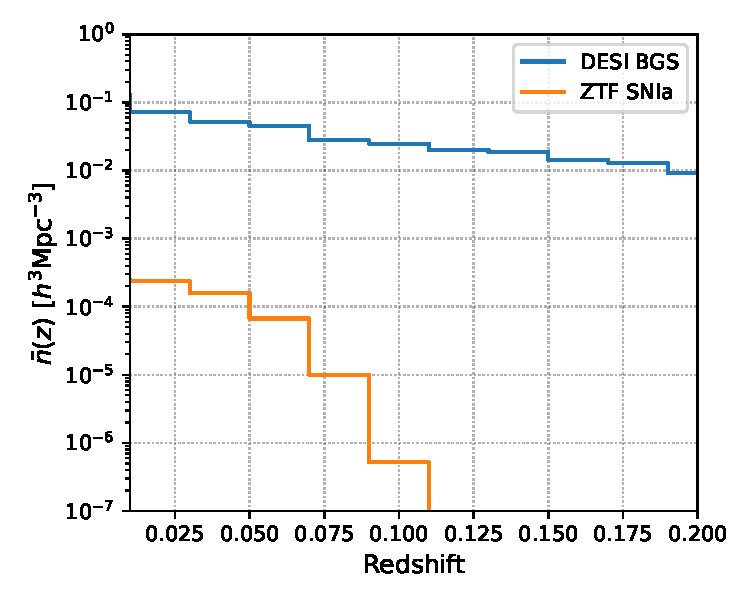
\includegraphics[width=0.5\textwidth]{fig/velocities/nz_desi_ztf.pdf}
    \caption{Comoving density of tracers as a function of redshift for the galaxies of 
    the DESI Bright Galaxy Survey (blue) and for type-Ia supernovae from ZTF (orange).
    Densities were computed assuming a flat $\Lambda$CDM model with 
    Planck 2018 best-fit parameters, based on simulated data and scaled to 
    match numbers expected at the end of both programs. 
    Both samples overlap in redshift and in sky coverage, which is ideal for joint studies 
    of densities and peculiar velocities. 
    }
    \label{fig:nz_desi_ztf}
\end{figure}


I studied the constraining power of DESI BGS and ZTF SNIa using the Fisher formalism.
I computed the uncertainty expected on $f\sigma_8$ from a RSD analysis with DESI BGS galaxies by themselves  
or from a joint RSD + PV analysis of DESI BGS and ZTF SNIa. 
I employed the same Fisher forecast code\footnote{\url{https://github.com/CullanHowlett/PV_fisher}} 
described in \cite{howlettMeasuringGrowthRate2017}. 
The inputs of the calculation are the expected comoving density of tracers for galaxies and peculiar velocities
at the end of both surveys, 
the intrinsic scatter of the distance indicators parametrised by $\alpha \equiv \sigma(D_L)/D_L \sim $10 or 20\%, 
and the scale range (in Fourier space) assumed for the measurement parametrised by $k_\text{max} \sim 0.1$ or $0.2~h\text{Mpc}^{-1}$. 
The model for the galaxy clustering is a simple linear RSD model with galaxy bias $b$ and 
a Gaussian Fingers-of-God term function of a galaxy velocity dispersion $\sigma_v$. 
The model for the velocity correlations is similar, scaling with $f$, but with a different 
empirical correction for the fact we observe velocities in redshift-space  (\cite{kodaArePeculiarVelocity2014}).
This empirical function depends on an extra dispersion parameter $\sigma_u$. 
A total of four free parameters define the model. I focused on the constraints on $f\sigma_8$ 
by using tracers over $0< z < 0.1$, which corresponds to a measurement at an effective 
redshift $z_\text{eff} = 0.08$. 

Results of the Fisher forecast are shown in Table~\ref{tab:forecast_fs8}
for different samples and analysis choices. 
First, we can see how the uncertainties on $f\sigma_8$ are 
significantly reduced when including ZTF SNIa, particularly when 
the intrinsic scatter is small and when using a larger range of scales. 
We see an improvement of a factor of 2.3 at most.  
Second, we see how increasing the scale range $k_\text{max}$ also improves contraints. 
This is why it is important to be able to model the clustering of galaxies and 
peculiar velocities on non-linear scales. 
Third, we see how improving the standardisation of SNIa also helps 
reducing uncertainties on $f\sigma_8$. 
In conclusion, a simple Fisher forecast predicts a 9\% measurement of $f\sigma_8$ 
in the optimistic scenario and a 20\% in the pessimistic scenario. 

\begin{table}
    \centering 
    \caption{Fisher forecast on measurements of the growth-rate of structures times the normalisation of the power spectrum 
    $f\sigma_8(z_\text{eff}) = 0.45$ where $z_\text{eff} = 0.08$ for the complete samples of DESI BGS and ZTF type-Ia supernovae. 
    Results are shown for different analysis choices: $k_\text{max}$ is the maximum wavenumber used in the analysis, 
    $\sigma(D_L)/D_L$ is the fractional error on luminosity distances due to intrinsic scatter. 
    The assumed number densities of tracers is the one shown in Figure~\ref{fig:nz_desi_ztf}. 
    The total assumed sky area with overlapping coverage from both experiments is 14k deg$^2$.
    }
    \label{tab:forecast_fs8}
    \begin{tabular}{lccc}
\hline 
\hline 
Dataset   & $k_\text{max}$  &  $\sigma(D_L)/D_L$  &     $\sigma \left(f\sigma_8(z_\text{eff})\right)/f\sigma_8(z_\text{eff})$ \\ 
\hline
DESI BGS  &  0.1 &  - &  0.58 \\
DESI BGS  &  0.2 &  - &  0.21 \\
ZTF SNIa  &  0.1 &  0.05 &  0.22 \\
ZTF SNIa  &  0.1 &  0.10 &  0.35 \\
ZTF SNIa  &  0.2 &  0.05 &  0.19 \\
ZTF SNIa  &  0.2 &  0.10 &  0.32 \\
DESI BGS + ZTF SNIa  &  0.1 &  0.05 &  0.12 \\
DESI BGS + ZTF SNIa  &  0.1 &  0.10 &  0.20 \\
DESI BGS + ZTF SNIa  &  0.2 &  0.05 &  0.09 \\
DESI BGS + ZTF SNIa  &  0.2 &  0.10 &  0.13 \\
\hline
\hline
    \end{tabular}
\end{table}


\section{Growth-rate measurement from simulated ZTF data}
\label{velocities:ztf_fs8}

Bastien Carreres, PhD student I co-supervise with Benjamin Racine and Dominique Fouchez at CPPM, 
is currently developing the whole analysis chain to measure the growth-rate of structures 
from peculiar velocities derived from ZTF type-Ia supernovae (SNIa) data. 
He has been developing a code based on the maximum-likelihood method 
(section~\ref{velocities:methods:maximum_likelihood}) and validating it with 
the most realistic set of simulated ZTF data that he also produced. 
In this section, I summarise his findings which will be detailed in 
Carreres et al. (in prep). 

\subsection{Simulating ZTF type-Ia supernovae with peculiar velocities}
\label{velocities:ztf_fs8:sims}

The goal of the simulations is to create a set of light-curves from SNIa 
which contain realistic and correlated peculiar velocities. 

The best source of peculiar velocities are n-body simulations. 
We currently use two sets of large-scale cosmological n-body simulations 
with matter only. The first set is named Dark Energy and Massive Neutrino Universe 
(DEMNUni, \cite{castorinaDEMNUniClusteringLargescale2015}) aimed at account correctly for 
the impact of massive neutrinos in the formation of structures. 
They were produced with the tree particle mesh-smoothed particle hydrodynamics 
(TreePM-SPH) code Gadget-3 with a recipee given by \cite{vielEffectNeutrinosMatter2010} 
to simulate massive neutrinos. The DEMNUni boxes are 2 $h^{-1}$Gpc on a side, 
and contain 2048$^3$ matter particles and $2048^3$ neutrino particles. Initial conditions 
are set at $z=99$ and evolved assuming a flat $\Lambda$CDM universe with parameters 
from Planck 2013 results (\cite{planckcollaborationPlanck2013Results2014a}). 
Different simulations were ran with varying mass of neutrino species (0, 0.16, 0.32, and 0.48 eV)
and varying equations-of-state for dark energy. 
Haloes were defined using a Friend-of-friends algorithm, assembling a minimum number of 32 
matter particles. This first set of simulations is not yet public and access it only granted 
by demand to the authors. 
The second set of simulations we use are the AbacusSummit suite (\cite{maksimovaABACUSSUMMITMassiveSet2021}), 
which use the Abacus code (\cite{garrisonABACUSCosmologicalNbody2021}) to produce 
150 boxes of 2 $h^{-1}$Gpc on a side, containing 6912$^3$ particles and 
spanning 97 cosmological models. These cosmological models have different 
values for $\omega_b$, $\omega_\text{cdm}$, $h$, $A_s$, $n_s$, $\alpha_s$, 
$N_\text{eff}$, $w_0$ and $w_a$. Initial conditions are created using 
first order Lagrangian perturbation theory with the public code
\textsc{zeldovich-PLT}\footnote{\url{https://github.com/abacusorg/zeldovich-PLT}}.
Halos are found using the CompaSO tehcnique (\cite{hadzhiyskaCOMPASONewHalo2022}).
These simulations and several data products are publicly available and 
documented\footnote{\url{https://abacussummit.readthedocs.io/}}. 
The AbacusSummit suite is currently the state-of-the-art in the market 
and are currently being used by the DESI collaboration. 

ZTF observes spectroscopically classified SNIa 
up to redshifts of 0.1, which corresponds to a comoving distance 
of $\sim 293$\hmpc in a Planck 2018 best-fit cosmology. 
This means that we can subdivide a $(2~h^{-1}\text{Gpc})^3$ simulation box into 
roughly 9 ZTF SNIa volumes (full-sky, even though ZTF observes the Northern sky).  
Because of large-scale correlations, these sub-boxes are not completely independent of each other. 
We place the observer at the center of each sub-box and compute the radial 
component of peculiar velocities for each halo. 
Eventually we convert comoving distances into redshifts assuming a fiducial cosmology. 
At this step, we can also include the effect of redshift-space distortions (RSD) using the radial velocities.
Currently we do not apply any halo mass cuts in our halo samples. 

With halo samples in hand, we randomly assing SNIa events following a given rate of 
events per volume, e.g., $(2.35 \pm 0.24) \times 10^4 \text{Gpc}^{-3} \text{yr}^{-1}$ 
(\cite{perleyZwickyTransientFacility2020}).
Using observation logs from real ZTF observations, we can know which exposures 
could observe our SNIa events within some time window comparable to the duration of 
a SNIa light-curve. For each observed SNIa, we draw strech and colour parameters 
defined as in the SALT2 formalism (\cite{guySALT2UsingDistant2007}) and following 
realistic distributions
(\cite{scolnicMEASURINGTYPEIA2016, nicolasRedshiftEvolutionUnderlying2021}).
Intrinsic scatter is added by hand on the peak magnitudes. 
The fluxes are simulated using the \textsc{SNCosmo} package\footnote{\url{https://sncosmo.readthedocs.io/}}.
Each exposure contains information about the seeing, airmass, and noise, which are then combined 
to obtain fluxes and their uncertainties. 
The peculiar velocity information is included in the observed redshift of the SNIa event
and accounted for when deriving fluxes in each band. 

Once light-curves are computed for all observed SNIa, we simulate 
selection effects. First, we define a photometric cut to emulate detection.
We exclude any light-curve without two epochs with flux signal-to-noise ratio 
above 5. Second, we emulate the spectroscopic follow-up for classification.
The selection for spectro follow-up is essentially a magnitude cut (roughly $r<18.5$),
which ensures enough signal in spectra.  
This second cut is the main responsible for the limit of $z \sim 0.1$ of the SNIa sample 
as seen in Figure~\ref{fig:nz_desi_ztf}. 
A mock ZTF SNIa sample with peculiar velocities is the result of this procedure. 
The package producing these mock catalogues is publicly 
available and documented\footnote{\url{https://snsim.readthedocs.io/}}. 

\section{Measuring peculiar velocities and the growth-rate}
\label{velocities:ztf_fs8:measurements}

With a realistic mock catalogue of ZTF SNIa data in hand, we proceed to the measurement of 
their peculiar velocities and the estimate of the growth-rate of structures $f\sigma_8$. 

Figure~\ref{fig:ztf_snsim_lightcurves} shows a few examples of light-curves from mock ZTF data.
These light-curves are then fitted with the same SALT2 models used to produce them. 
The fits yield values for the stretch, colour, peak brightness and the time of peak brightness, 
with their uncertainties. 
A Hubble diagram is fitted including terms accounting for correlations between brightness and 
stretch/colour (Tripp relation). 
Since we are at such low redshifts, we can model $H(z)$ as a linear function since 
the cosmological dependency with $\Omega_m$ or $\Omega_\Lambda$ only kicks in at $z \sim 0.4$, 
much higher than our sample. 
The peculiar velocity estimator uses the residuals of the observed distance moduli to the
best-fit Hubble diagram. While most of the displacements due to velocities happen in the redshift direction,
the noise is much larger in the distance moduli diretion, so the most convient observable is 
the Hubble residual $\Delta \mu \equiv \mu_\text{obs} - \mu_\text{model}(z_\text{obs})$. 
Using a linear expansion of the Hubble diagram, one can write an approximation of the corresponding 
peculiar velocity, though its noise properties become non-Gaussian. Therefore most studies 
simply use $\Delta \mu$ as the peculiar velocity observable. 


\begin{figure}
    \centering
    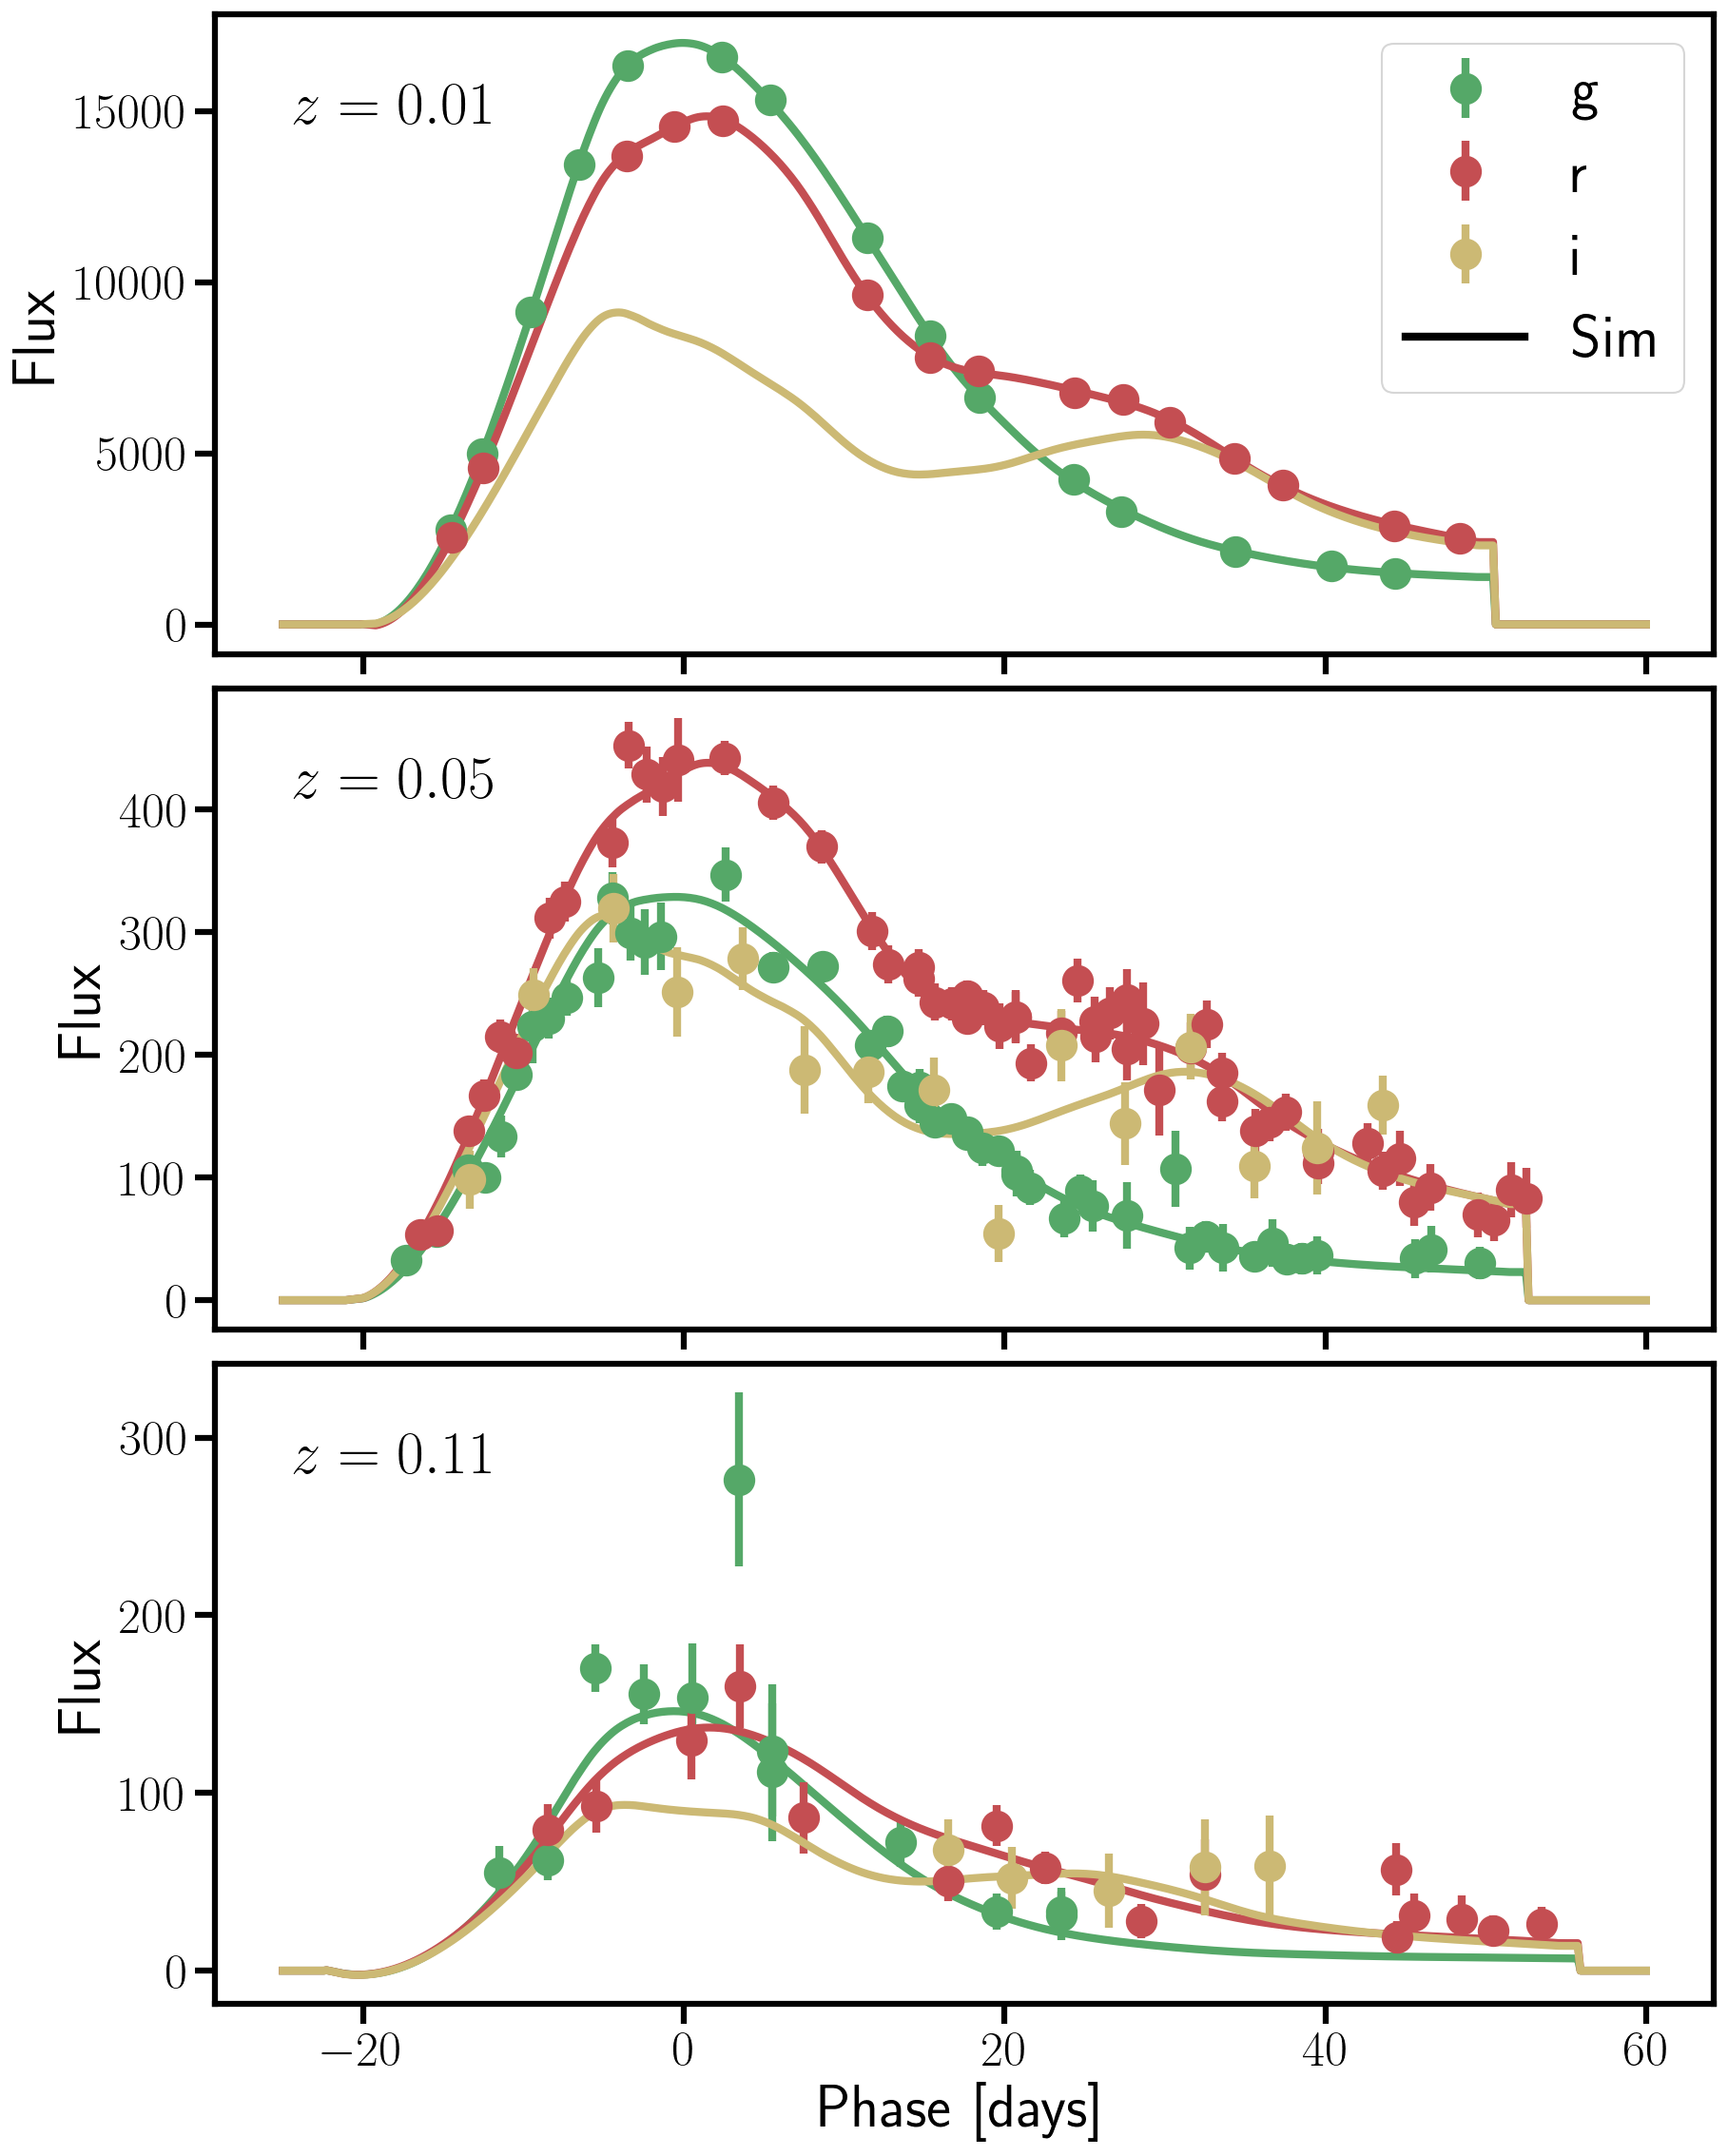
\includegraphics[width=0.6\textwidth]{fig/velocities/snsim_lightcurves.png}
    \caption{Three simulated type-Ia supernovae light-curves as observed by ZTF, ranging from low to mid and high redshift. 
    The solid line represents the input light-curve model while points with errorbars are simulated observed fluxes 
    including instrumental noise. The flux is in arbitraty units. Figure extracted from Carreres et al. (in prep). }
    \label{fig:ztf_snsim_lightcurves}
\end{figure}

Figure~\ref{fig:ztf_snsim_hubble_diagram} displays the residuals of the Hubble diagram 
fitted on simulated samples of ZTF light-curves, relative to the true input Hubble diagram. 
The average of eight independent realisations is also displayed with errorbars. 
A clear bias relative to the input model is seen at $z > 0.06$, 
due mainly to the selection for spectroscopic follow-up. 
If the simulations are realistic enough, this bias is an indication that ZTF SNIa samples 
are \emph{complete} up to $z \sim 0.06$, defining a so called \emph{volume limited} sample. 
Above this limit, we need to correctly 
account for biases if one is interested in constraining cosmology with the Hubble diagram. 
In this work, we studied the impact of this selection bias in the measurement of peculiar 
velocities and subsequently on the estimates of the growth-rate $f\sigma_8$.  

\begin{figure}
    \centering
    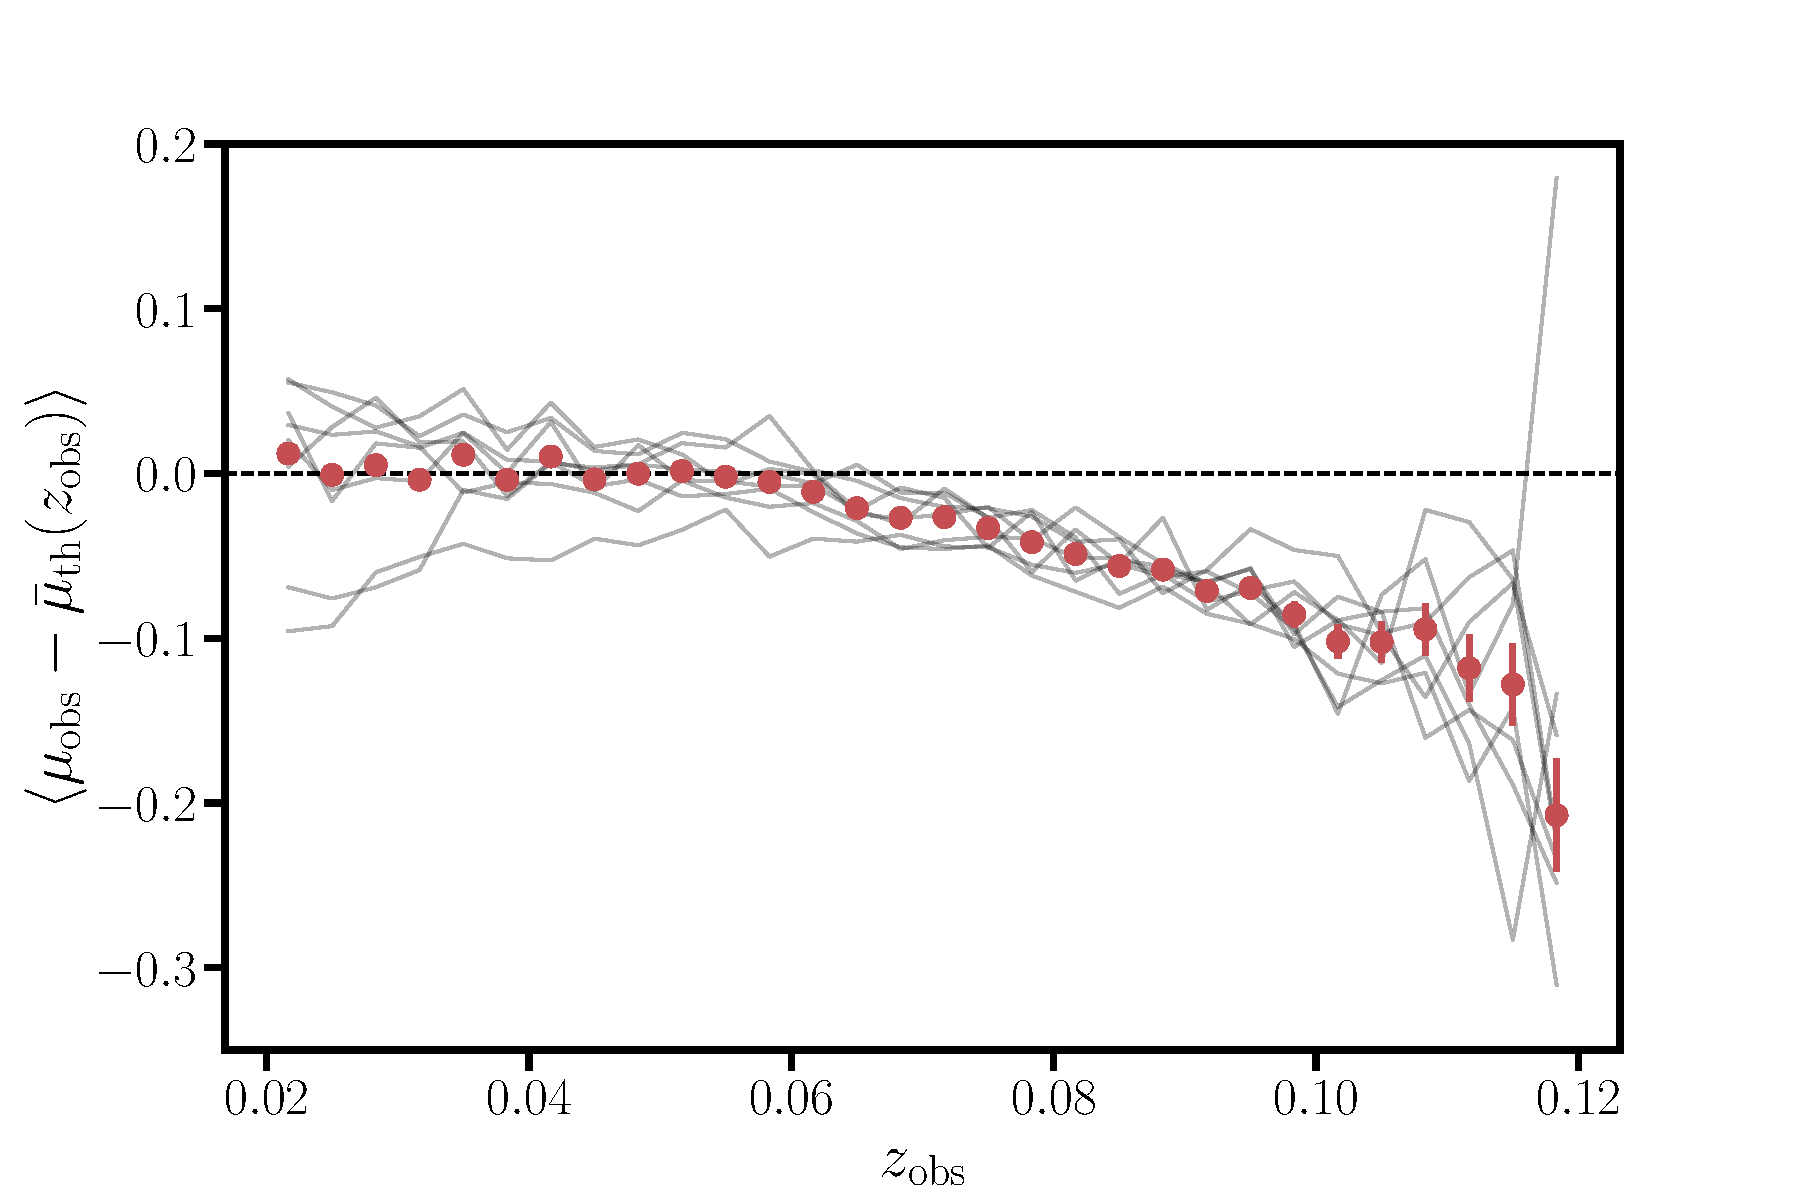
\includegraphics[width=0.6\textwidth]{fig/velocities/bastien_hd_residuals.pdf}
    \caption{Distance moduli inferred from simulated ZTF SNIa light-curves compared to the input cosmological model. 
    Grey lines show 8 different realisations while points with error bars are their average. 
    Selection effects cause a bias in distance moduli estimates at $z>0.06$. 
    Figure extracted from Carreres et al. (in prep).}
    \label{fig:ztf_snsim_hubble_diagram}
\end{figure}

For our measument of $f\sigma_8$ using peculiar velocities, we are currently employing 
the maximum-likelihodd method (section~\ref{velocities:methods:maximum_likelihood}). 
Instead of using a linear matter power spectrum as a model for the velocity divergence 
power spectrum, we are trying to use improved models including regularised perturbation 
theory (RegPT, \cite{taruyaDirectFastCalculation2012}) and empirical formulas derived
from n-body simulations (\cite{belAccurateFittingFunctions2019}). 
These models include some level of non-linearities which would allow us to use 
a larger range of scales when constraining growth. Also, linear theory is knwon to break 
at quite large scales $k\sim 0.1$, particularly at $z\sim0$. 

When building the model covariance matrix used in the likelihood (Eq.~\ref{eq:likelihood})
for $N_v$ measurements of peculiar velocities, the resulting matrix will have $N_v^2$ elements, 
which can become prohibitively large and slow to compute. We expect that ZTF will produce a set 
of about 5000 SNIa which is still feasible, but larger sets require a different solution. 
One of the solutions is to assign the velocities to a mesh, effectively reducing the number of 
measurements. This also has the advantage of smoothing out a fraction of the non-linear clustering. 
The mesh smoothing is taken into account in the model covariance matrix. 

There are three free parameters in the model covariance matrix: $f\sigma_8$ which is simply to overall 
amplitude of velocity-velocity correlations, $\sigma_v$ accounting for the remaining non-linear 
velocities, $\sigma_u$ accouting for the change in the signal due to redshift-space distortions. 
We use the \textsc{iMinuit} package\footnote{\url{https://iminuit.readthedocs.io/}} to find the maximum 
of the likelihood and to estimate uncertainties. We also explore the full posterior distribution 
using a Monte Carlo Markov Chain (MCMC). 

Figure~\ref{fig:ztf_snsim_posterior} shows one example of the posterior on the three fitter parameters. 
In order to avoid selection biases, we restrain our dataset to SNIa at $z<0.06$, 
which yields about 2000 objects for this case.
Contours show the 68 and 95\% confidence levels. Green contours are the result of analysing the 
peculiar velocities directly from the halo catalogue, without any source of noise. Red contours 
are the result when including all the effects of a realistic dataset and analysis. 
Both measurements are consistent with the expected value for $f\sigma_8$, even though uncertainties 
are quite large.

\begin{figure}
    \centering
    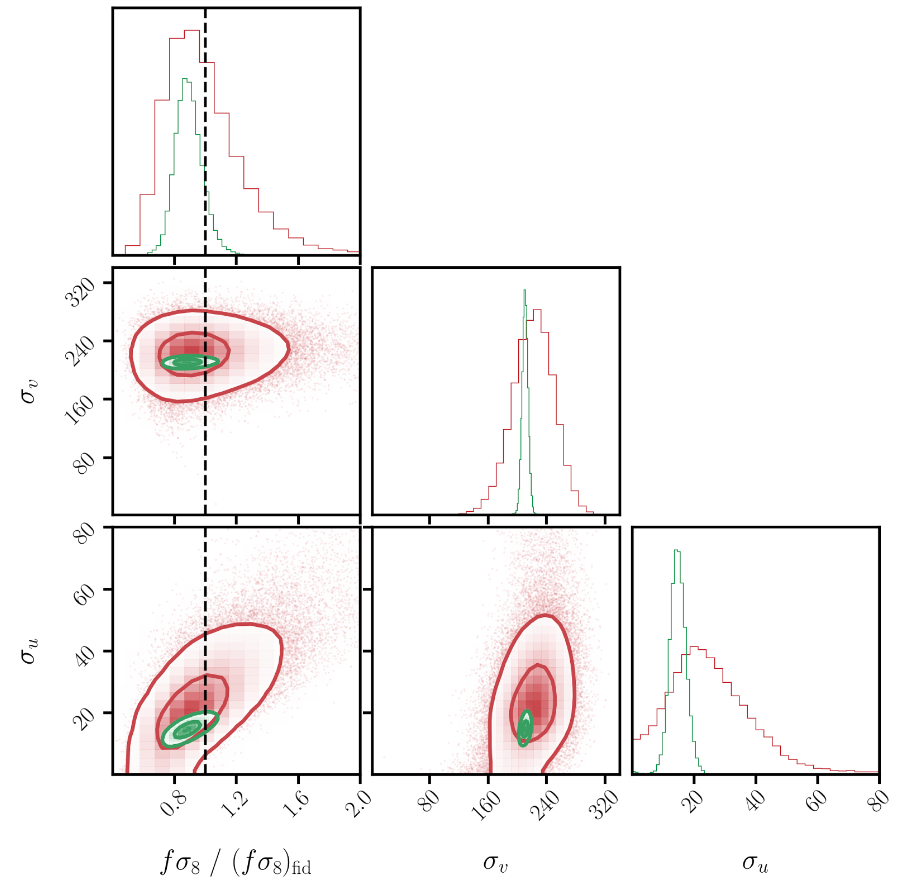
\includegraphics[width=0.6\textwidth]{fig/velocities/bastien_posterior_fs8.png}
    \caption{ Figure extracted from Carreres et al. (in prep).}
    \label{fig:ztf_snsim_posterior}
\end{figure}

Figure~\ref{fig:ztf_snsim_fs8_bias} shows how best-fit values of $f\sigma_8$ change when 
increasing the dataset up to $z_\text{max}$. We clearly see the impact of selection biases 
when considering SNIa beyond $z\sim 0.08$, based on the average of 8 mock realisations. 
This would indicate that an unbiased measurement of $f\sigma_8$ is possible with ZTF SNIa
if one restricts the analysis to the volume limited sample. 
Another interesting result is that the uncertainty in $f\sigma_8$ does not seem to 
decrease significantly when increasing $z_\text{max}$. This is simply a manifestation 
of the quick fall in the comoving density of SNIa beyond $z\sim0.08$, as seen in 
Figure~\ref{fig:nz_desi_ztf}. 
Also in the same redshift range, a large set of DESI galaxies will be available to 
perform a joint density-velocity analysis. 

\begin{figure}
    \centering
    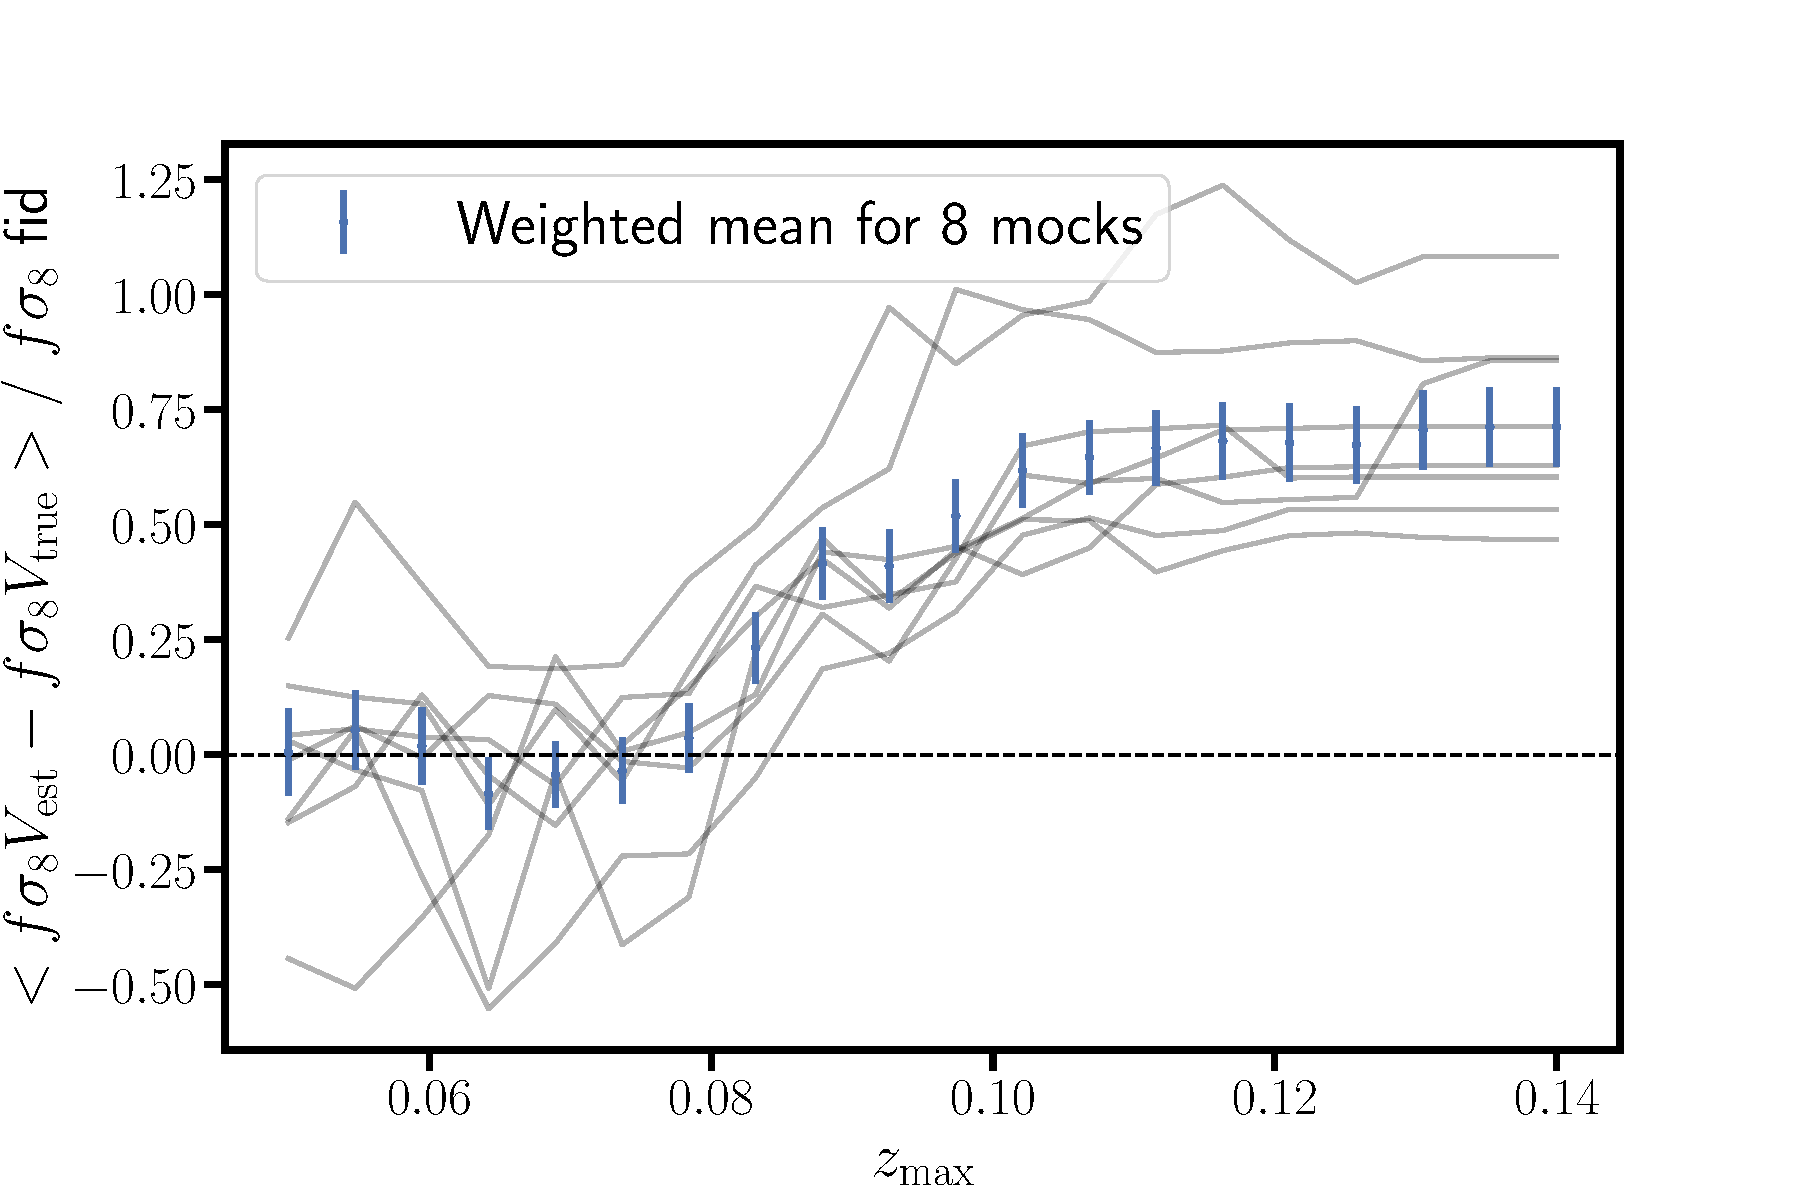
\includegraphics[width=0.6\textwidth]{fig/velocities/bastien_fs8_bias.pdf}
    \caption{Estimates of the growth-rate $f\sigma_8$ from mock ZTF SNIa data. 
    We compare the measurements between the estimated peculiar velocities to the 
    same measurements performed on the true velocities. 
    Each measurement considers SNIa up to maximum redshift $z_\text{max}$.
    The selection bias from Figure~\ref{fig:ztf_snsim_hubble_diagram} manifests itself
    on growth-rate estimates from $z_\text{max}>0.08$. 
    Figure extracted from Carreres et al. (in prep).}
    \label{fig:ztf_snsim_fs8_bias}
\end{figure}



	\chapter*{Conclusion}
	\addcontentsline{toc}{chapter}{Conclusion}
	\lipsum[1-2]

	\appendix

	\newpage
	\printbibliography[					%% bibliographie
	heading=bibintoc
	]	
	% \newpage
	% \printindex							%% index
	% \newpage
	% \printendnotes						%% notes

	%% annexes
	%\setcounter{chapter}{0}
	%\renewcommand{\thesection}{\Alph{section}}
	
	%\chapter*{Appendix}
	%\newpage
	%\addcontentsline{toc}{chapter}{Appendix}
	
	%\section{Intitulés des doctorats AMU}
\label{chap:doctorats}

		\begin{itemize}
		\item Discipline
			\begin{itemize}
			\item Spécialité
			\end{itemize}
		\end{itemize}
		
	\subsection*{ED 62 SCIENCES DE LA VIE ET DE LA SANTE}\label{ed-62-sciences-de-la-vie-et-de-la-sante}

		\begin{itemize}
		\item Biologie santé
			\begin{itemize}
			\item Biochimie structurale
			\item Génomique et  Bioinformatique
			\item Biologie du développement
			\item Immunologie
			\item Génétique
			\item Microbiologie
			\item Biologie végétale
			\item Neurosciences
			\item Oncologie
			\item Maladies infectieuses
			\item Pathologie vasculaire et nutrition
			\item Ethique
			\item Recherche clinique et Santé Publique
			\item Biotechnologie
			\end{itemize}
		\end{itemize}

	\subsection*{ED 67 SCIENCES JURIDIQUES ET POLITIQUES}\label{ed-67-sciences-juridiques-et-politiques}

		\begin{itemize}
		\item Droit
			\begin{itemize}
			\item Droit Privé
			\item Droit Public
			\item Histoire du Droit
			\end{itemize}
		\item Science Politique
		\end{itemize}

	\subsection*{ED 184 MATHEMATIQUES ET INFORMATIQUE}\label{ed-184-mathematiques-et-informatique}

		\begin{itemize}
		\item Mathématiques
		\item Informatique
		\item Automatique
		\end{itemize}

	\subsection*{ED 250 SCIENCES CHIMIQUES DE MARSEILLE}\label{ed-250-sciences-chimiques-de-marseille}

		\begin{itemize}
		\item Sciences Chimiques
		\end{itemize}

	\subsection*{ED 251 SCIENCES DE L'ENVIRONNEMENT}\label{ed-251-sciences-de-lenvironnement}

		\begin{itemize}
		\item Sciences de l'Environnement
			\begin{itemize}
			\item Anthropologie biologique
			\item Ecologie
			\item Géosciences 
			\item Génie des procédés
			\item Océanographie
			\item Chimie 
			\item Environnement et santé 
			\end{itemize}
		\end{itemize}

	\subsection*{ED 352 PHYSIQUE ET SCIENCES DE LA MATIERE}\label{ed-352-physique-et-sciences-de-la-matiere}

		\begin{itemize}
		\item Physique et Sciences de la Matière 
			\begin{itemize}
			\item Astrophysique et Cosmologie
			\item Biophysique
			\item Energie, Rayonnement et Plasma
			\item Instrumentation
			\item Optique, Photonique et Traitement d'Image
			\item Physique des Particules et Astroparticules
			\item Physique Théorique et Mathématique
			\item Matière Condensée et Nanosciences 
			\end{itemize}
		\end{itemize}

	\subsection*{ED 353 SCIENCES POUR L'INGENIEUR: MECANIQUE, PHYSIQUE, MICRO ET NANOELECTRONIQUE}\label{ed-353-sciences-pour-lingenieur-mecanique-physique-micro-et-nanoelectronique}

		\begin{itemize}
		\item Sciences pour l'Ingénieur
			\begin{itemize}
			\item Energétique
			\item Mécanique et physique des fluides 
			\item Acoustique
			\item Mécanique des solides
			\item Micro et Nanoélectronique
			\item Génie civil et architecture
			\item Nucléaire de fission 
			\item Fusion magnétique
			\end{itemize}
		\end{itemize}

	\subsection*{ED 354 LANGUES, LETTRES ET ARTS}\label{ed-354-langues-lettres-et-arts}

		\begin{itemize}
		\item Etudes anglophones
		\item Etudes germaniques
		\item Etudes slaves
		\item Langues et littératures d'Asie
			\begin{itemize}
			\item Chinois
			\item Vietnamien
			\item Coréen
			\end{itemize}
        	\item Arts
            		\begin{itemize}
            		\item Arts plastiques 
            		\item Sciences de l'art
            		\item Musique et musicologie
            		\item Etudes cinématographiques et audiovisuelles
            		\item Arts de la scène
            		\item Médiation culturelle des arts
            		\end{itemize}
        	\item Pratique et théorie de la création artistique et littéraire
		\item Langue et Littératures françaises
		\item Littérature générale et comparée
		\item Langues, littératures et civilisations romanes 
			\begin{itemize}
			\item Etudes hispaniques et latino-américaines
			\item Etudes italiennes
			\item Etudes roumaines
			\end{itemize}
		\end{itemize}

	\subsection*{ED 355 ESPACES, CULTURES, SOCIETES}\label{ed-355-espaces-cultures-societes}

		\begin{itemize}
		\item Géographie
		\item Urbanisme et Aménagement du territoire
		\item Préhistoire
		\item Archéologie
		\item Histoire de l'Art
		\item Histoire
		\item Sciences de l'Antiquité
		\item Mondes arabe, musulman et sémitique
		\item Etudes romanes
		\item Sociologie
		\item Anthropologie
		\item Architecture
		\item Cultures et Sociétés d'Asie
		\end{itemize}

	\subsection*{ED 356 COGNITION, LANGAGE, EDUCATION}\label{ed-356-cognition-langage-education}

		\begin{itemize}
		\item Philosophie
		\item Psychologie
		\item Sciences du Langage
		\item Sciences de l'Information et de la Communication
		\item Sciences de l'Education
		\item Sciences Cognitives
		\end{itemize}

	\subsection*{ED 372 SCIENCES ECONOMIQUES ET DE GESTION}\label{ed-372-sciences-economiques-et-de-gestion}

		\begin{itemize}
		\item Sciences de Gestion
		\item Sciences Economiques
		\end{itemize}

	\subsection*{ED 463 SCIENCES DU MOUVEMENT HUMAIN}\label{ed-463-sciences-du-mouvement-humain}

		\begin{itemize}
		\item Sciences du Mouvement Humain 
		\end{itemize}

	%\newpage
	%\section{Données brutes}

	\lipsum[1-4]


\end{document}
